% Tipo de documento
\documentclass[12pt, twoside, a4paper, openany, bibliography=totoc]{scrbook}

% Añadir caracteres no anglosajones como tildes, ñ, ¿, ¡, etc.
\usepackage[utf8]{inputenc}
\usepackage[spanish]{babel}
 
% Añadir gráficos
\usepackage{graphicx}
% Carpeta donde se encuentran las imágenes
\graphicspath{ {figs/} }
\usepackage{caption}
\usepackage{subcaption}
\DeclareGraphicsExtensions{.pdf,.png,.jpg}
\usepackage{chngcntr}
\counterwithout{figure}{chapter}

% Listas con corchetes tipo [1], [2]...
\usepackage{enumitem}

% Permite usar hipervínculos
\usepackage[hidelinks]{hyperref}

\usepackage{afterpage}

\newcommand\blankpage{
    \null
    \thispagestyle{empty}
    \newpage}

% Floating options
\usepackage{float}
\restylefloat{figure}

% Márgenes
\usepackage[left=2.5cm,right=2.5cm,bindingoffset=0.5cm]{geometry}

% Fuente utilizada para el cuerpo
\usepackage[bitstream-charter]{mathdesign}

% Permite usar frames (cajas)
\usepackage{framed}

% Permite usar colores
\usepackage[usenames,dvipsnames,svgnames,table]{xcolor}

% Permite el uso de cabeceras y pies de página
\usepackage{fancyhdr}

% Biblatex
\usepackage[backend=bibtex,style=numeric,natbib=true]{biblatex}
\addbibresource{bibliography.bib}

% Permite realizar rotaciones
\usepackage{rotating}

% Opciones de tablas
% Para crear líneas más gruesas
\usepackage{tabu}
\counterwithout{table}{chapter}

\captionsetup[figure]{font=bf,position=below}

\begin{document}

\fancyhead[R]{\slshape \rightmark}
\fancyfoot[C]{\thepage}

% Permite escoger la profundidad de las secciones (1.1, 1.1.1.2...)
\setcounter{secnumdepth}{2}

%----------------------------------------------------%
%                      PORTADA                       %
%----------------------------------------------------%

% No mostrar número de página
\pagestyle{empty}

% Define una linea horizontal para el titulo
\newcommand{\HRule}{\rule{\linewidth}{0.5mm}} 

% Centra el contenido
\begin{center}
	% Titulo entre dos líneas horizontales
	\HRule \\[0.5cm]
	\vspace{0.5cm}
	\textbf {
		{\huge exerClick}\\
		\vspace{0.3 cm}
		Aplicación para el seguimiento de ejercicios en el aula\\
	}
	\vspace{0.5cm}
	\HRule \\[2.0cm]
	{\large
		1 de septiembre de 2015\\
		\vspace{2.0 cm}
		Autor:\\
		Adrián Núñez Marcos\\
		\vspace{1.0 cm}
		Directora:\\
		Maite Urretavizcaya Loinaz\\
	}

	\vspace{2.0 cm} 
	\begin{figure}[h!]
		\centering
		
\includegraphics[width=0.4\textwidth]{ehu.pdf}\hfill
		
\includegraphics[width=0.4\textwidth]{informatika.pdf}
	\end{figure}
\end{center}

\frontmatter
\pagestyle{plain}
\cleardoublepage

%----------------------------------------------------%
%                  AGRADECIMIENTOS                   %
%----------------------------------------------------%

\begin{flushright}
	\Large\textit{Dedicado a...}
\end{flushright}

\vspace{1.0 cm}

Introducir los agradecimientos aquí.
\cleardoublepage

%----------------------------------------------------%
%                      RESUMEN                       %
%----------------------------------------------------%

% Castellano
% No mostrar número de página
\pagestyle{empty}

\section*{Resumen}

Proyecto de Fin de Grado de la especialidad de Computación. Se ha implementado la aplicación para el seguimiento de ejercicios en el aula llamada exerClic. Es una aplicación para móviles libre de plataforma, habiendo sido adaptada a Android y a iOS, gracias a la plataforma Cordova. En su implementación se han utilizado las tecnologías web HTML5, CSS3 y Javascript, además de PHP para el servidor.\\

La aplicación permite que los profesores añadan ejercicios y los alumnos le envíen \textit{feedback} sobre su realización mediante dos opciones: marcar una duda en el ejercicio o marcar el ejercicio como finalizado.\\
\cleardoublepage

% Euskera
\section*{Laburpena}

Sartu hemen laburpenaren textua\\
\cleardoublepage

% Inglés
% No mostrar número de página
\pagestyle{empty}

\section*{Abstract}

Put here the text for the abstract\\
\cleardoublepage

%----------------------------------------------------%
%                    INDICE GENERAL                  %
%----------------------------------------------------%

\tableofcontents
\newpage

%----------------------------------------------------%
%                    INDICE FIGURAS                  %
%----------------------------------------------------%

\listoffigures
\newpage

%----------------------------------------------------%
%                    INDICE TABLAS                   %
%----------------------------------------------------%

\listoftables
\cleardoublepage

%----------------------------------------------------%
%                    INTRODUCCION                    %
%----------------------------------------------------%

\mainmatter
%----------------------------------------------------%
%                    INTRODUCCION                    %
%----------------------------------------------------%

\pagestyle{fancy}

\chapter{Introducción}
\label{introduccion}

\section{Contexto}

Muchas veces nos encontramos con aulas con demasiados alumnos. Estas clases son especialmente comunes en los primeros cursos de los estudios universitarios, donde el número de alumnos alcanza fácilmente las tres cifras. Conocer todos los alumnos que tienen dudas y monitorizar a los alumnos para saber si todos o la mayoría han acabado el ejercicio son tareas difícilmente abordables por una sola persona. La mayoría de las veces se suelen ignorar los problemas y dudas, y se sigue adelante.\\

Los nuevos planes de estudio que pretenden dejar atrás el sistema de educación mediante clases magistrales y dinamizar las clases han supuesto un aumento en el número de clases prácticas y laboratorios que se realizan. Algunos centros han optado incluso por dividir las clases en grupos más pequeños para realizar las prácticas, pero muchas veces ésto no es posible. En esas situaciones el profesor acaba por no poder monitorizar completamente la clase.\\

Con el fin de tener un medio común se han implantado en los últimos años nuevas tecnologías en entornos docentes. Sin embargo, en muchos casos esta tecnología se limita a entornos de apoyo a la docencia más que al alumnado, siendo muy popular el sistema de gestión del aprendizaje Moodle. Además, el uso más frecuente de estos sistemas es el de simple almacén de recursos bibliográficos (enlaces, apuntes, transparencias, etc.).\\

Por otro lado, la expansión de las tecnologías móviles y tabletas, con las que los alumnos están cada vez más familiarizados, no ha sido aprovechada. Estas tecnologías están ya mayoritariamente presentes en las aulas, la mayoría del alumnado dispone de alguno de estos dispositivos, pero su uso como herramienta educativa no es real, desperdiciando así todo su potencial como sistema de ayuda al aprendizaje. Es más, muchas veces el uso de estos dispositivos está prohibido o limitado en clase.\\

\section{Propuesta}

Nuestra propuesta pretende modificar y actualizar los modelos educativos presenciales a través de herramientas que faciliten la captura de la información de lo que sucede en el aula, con el objetivo de proporcionar \textit{feedback} a profesores y estudiantes sobre su progreso en el aprendizaje. Esta propuesta se materializa en la aplicación PresenceClick que facilita la captura colaborativa de esta información entre alumnos y profesores de manera ágil. PresenceClick actualmente dispone de una serie de módulos que capturan la asistencia de los alumnos a clase de manera automática, sus sensaciones sobre las diversas actividades de aprendizaje, sus respuestas a preguntas al aire del profesor y sus dudas. En particular, nuestro objetivo en este nuevo proyecto es capturar las interacciones entre profesor-alumnos en sesiones de ejercicios.\\

El profesor dispondrá de una interfaz a la que accederá mediante su dispositivo móvil o tableta en clase e indicará a sus alumnos los ejercicios a realizar (está actividad se podrá realizar previa a la clase). Por su parte, los alumnos con sus dispositivos móviles (smartphones o tabletas) recibirán las notificaciones de los ejercicios a realizar y podrán indicar para cada uno si tienen dudas en su realización o si lo han terminado. El profesor podrá disponer en tiempo real de información sobre el porcentaje de alumnos que lo han realizado, alumnos que indican problemas en su realización y aquellos alumnos que no indican nada. Es decir, el profesor tendrá idea en tiempo real de quiénes y cuántos han realizado el ejercicio o alumnos que tienen problemas en su realización y podrá acercarse a comprobar y revisar sus soluciones. Además el profesor podrá valorar su nivel de corrección o satisfacción en la realización, añadiendo las notas oportunas en el sistema que le permitirá seguir la evolución de cada uno de sus alumnos durante el curso. También podrá acercarse a aquellos que señalan problemas en su realización, con el fin de ayudarlos y evitar dificultades en su progreso.\\

Bajo este contexto surge \textbf{exerClick}, la herramienta para seguimiento de ejercicios en el aula. Esta herramienta, con todas sus funcionalidades, nace con el propósito de tener una visión más real de lo que hacen los alumnos, tanto una visión global del grupo como una individual y está dirigida a profesores y a los propios alumnos. De esta manera, el docente puede ofrecer un aprendizaje más adaptado e individualizado, aunque los grupos de alumnos sean muy grandes.\\

\section{Organización del documento}

En este documento se describe principalmente la gestión y el seguimiento realizado durante el desarrollo de \textbf{exerClick}.\\

Introducir organización.\\

%----------------------------------------------------%
%                     OBJETIVOS                      %
%----------------------------------------------------%

%----------------------------------------------------%
%                     OBJETIVOS                      %
%----------------------------------------------------%

\pagestyle{fancy}

\chapter{Documento de objetivos del proyecto (DOP)}
\label{objetivos}

Durante las sesiones prácticas de ejercicios en el aula a menudo el docente se pregunta si todo el mundo ha acabado los ejercicios propuestos con la esperanza de poder continuar con otro ejercicio o dando las explicaciones necesarias para poder continuar. Se puede preguntar si sus alumnos tienen vergüenza de plantear dudas o si pasan de ello, si no estará consumiendo demasiado tiempo en este ejercicio, etc. Con un conjunto de 100 alumnos, por ejemplo, resulta imposible observar el avance de los alumnos en los ejercicios y atender a todas las dudas que surgen. Incluso la estrategia de dividir la clase en grupos más pequeños para las clases prácticas, que puede parecer una buena idea, acaba consumiendo más tiempo, al tener que repetir lo mismo varias veces.\\

Lo ideal sería que existiera un medio para permitir a los alumnos dejar claro el estado en el que se encuentran, que el profesor pudiera ver como va cada alumno y que si hubiera dudas quedaran en algún sitio almacenadas para no dejar a ningún alumno sin su respuesta.\\

Con estos objetivos nace exerClick, que pretender ayudar a alumnos y docentes a llevar a cabo esta tarea. En este capítulo describiremos el alcance del proyecto.\\

%----------------------------------------------------%
%                       ALCANCE                      %
%----------------------------------------------------%

\section{Alcance del proyecto}

Dividiremos los objetivos en objetivos del alumno y objetivos del profesor. Estos son los objetivos fijados para el alumno:

\begin{itemize}
\item Que pueda ver en todo momento cuales son los ejercicios propuestos en clase.
\item Que un alumno pueda dejar constancia del estado en el que se encuentra durante un ejercicio: si lo ha terminado, si tiene dudas o si está realizándolo.
\item Ver su progreso y el de sus compañeros en la realización de ejercicios.
\end{itemize}

Los objetivos del docente serán los siguientes:

\begin{itemize}
\item Que pueda ver en todo momento cuales son los ejercicios que va proponiendo en clase, los que se han terminado durante la sesión presente o los que aún no se han propuesto pero están preparados.
\item Crear en cualquier momento un nuevo ejercicio (rápidamente o bien preparándolo tranquilamente). Y una vez creado tener la posibilidad de proponerlo a la clase o guardarlo para proponerlo más tarde.
\item Ver por cada ejercicio el estado de los alumnos: quiénes lo han terminado, quiénes tienen duda y quiénes no han respondido nada.
\item Editar cualquier detalle de un ejercicio en cualquier momento.
\item Valorar la realización de un ejercicio a un alumno concreto.
\end{itemize}

Además, se han fijado dentro del alcance los siguientes requisitos:

\begin{itemize}
\item Contar con la opinión de usuarios finales (alumnos y docentes) durante el desarrollo de la aplicación, asegurando su aceptación general.
\item La internacionalización de la aplicación, que tendrá 4 idiomas disponibles: castellano, euskera, inglés y francés.
\item Desarrollar la aplicación para que funcione en el mayor número de dispositivos posibles: smartphones, tablets, etc., teniendo en cuenta los diferentes tamaños de pantalla.
\item La aplicación será multiplataforma, pudiendo funciona en Android, iOS y Windows Phone.
\end{itemize}


%----------------------------------------------------%
%                     EXCLUSIONES                    %
%----------------------------------------------------%

\section{Exclusiones del proyecto}

\begin{itemize}
\item Se van a excluir del proyecto todas las funciones que se puedan desarrollar en PresenceClick ligadas a exerClick (es decir, sobre ejercicios en el aula, como pueden ser estadísticas más trabajadas).
\end{itemize}


%----------------------------------------------------%
%              FASES Y TAREAS DEL PROYECTO           %
%----------------------------------------------------%

\section{Fases y tareas del proyecto}

\subsection{Estudio de alternativas para la creación de una aplicación móvil}

Al principio el proyecto iba a seguir a su antecesor, \textit{qClick}, como una aplicación web. Sin embargo, acabó pensándose durante una reunión inicial en convertirlo en una aplicación móvil para aprovecharse mejor de las ventajas de un móvil: notificaciones, no requiere necesidad de cargar la página cada vez que se entra, etc.\\

Ya que el proyecto iba a ser una aplicación web y por tanto se iban a usar tecnologías web se acordó usar un sistema como Apache Cordova para la implementación de la aplicación en lugar de crear una aplicación nativa. Así no se requerían de conocimientos de Android y por tanto se mantenían las bases iniciales del proyecto.\\

Se pensó en Apache Cordova ya que era conocido por uno de los integrantes del grupo GaLan, que estaba desarrollando una aplicación con esta tecnología. De esta forma se podía consultar en caso de alguna duda o pregunta en general directamente a dicha persona en lugar de perder excesivo tiempo buscando respuestas.\\

\subsection{Formación}

Ya se partía con una base propia de conocimiento en tecnologías web, por lo que no fue un gran problema.\\

Samara Ruíz fue la que aportó información sobre Responsive Web Design al inicio del proyecto para poder empezar a realizar las interfaces gráficas. No tenía conocimientos al respecto de esta herramienta y fue de gran ayuda una clase rápida introductoria.\\

Para aprender Apache Cordova se siguieron tutoriales encontrados en la red, tanto para crear la primera aplicación como para simulaciones y pruebas. Para algunas cosas también se consultó con el grupo GaLan en ciertos momentos.\\

\subsection{Documentación del proyecto}

La memoria del proyecto se empezó en una etapa temprana del proyecto. Se comenzó creando la plantilla de \LaTeX \ con todo lo necesario desde cero. La plantilla de la universidad resultaba algo incómoda de usar para cambiar algunos detalles, es por eso que se decidió crear una propia. Tras tener el estilo definido y los paquetes necesarios añadidos se realizó la estructura del documento, añadiendo sólo las cabeceras de cada sección, subsección, etc.\\

También al inicio se comenzó a realizar un seguimiento constante. Mediante Google Drive se iban manteniendo hojas de cálculo con cada tarea realizada, su duración y fecha, así como el cómputo total de horas por mes (y dentro de cada mes por iteraciones, si hubiera más de una). De esta forma plasmarlo más adelante fue una tarea muy sencilla.\\

La memoria no se desarrolló demasiado hasta que la aplicación empezaba a verse acabada, momento en el que empezó a tomar cuerpo con mucho contenido. Debido a que en abril se empezaron los estudios en el programa Erasmus en Alemania la memoria quedó completamente parado hasta junio, momento en el que se finalizó exitosamente.\\

\subsection{Presentación y Defensa del proyecto}

La presentación del proyecto se realizará en los meses de agosto y septiembre, momento en el que se dispondrá de todo el tiempo necesario. Se plantea realizar unas transparencias para una presentación de 30 minutos con previo ensayo con la directora del proyecto.\\

%----------------------------------------------------%d
%                 ANALISIS DE RIESGOS                %
%----------------------------------------------------%

\section{Análisis de riesgos}

En este punto se concretan dos riesgos que pueden dar problemas durante el proyecto y la solución encontrada para mitigarlos:\\

\subsection*{Programa Erasmus}

El mayor riesgo durante el proyecto es el cuatrimestre en el programa Erasmus desde el mes de abril al mes de agosto: se desconocen los eventos que puedan acontecer durante esos meses, si la carga lectiva de las asignaturas y trabajos impedirá el seguir con la memoria, o simplemente puede ser una mala época anímicamente hablando para realizar el proyecto. De cualquier modo, para evitar este riesgo se ha pensado en acabar la aplicación por lo menos antes de marchar para minimizar riesgos.\\

\subsection*{Pérdida de información}

La pérdida de información siempre es una posibilidad cuando se trabaja en una aplicación de esta índole. Para tener menos probabilidades de que se pierda absolutamente todo se realizan varias copias de todos los ficheros:

\begin{itemize}
\item Copia principal en el ordenador de trabajo.
\item En Github, en el repositorio exerClick (ver sección \ref{infraestructura}).
\item En Google Drive.
\end{itemize}

Se actualizan periódicamente, sin una frecuencia fija.\\

%----------------------------------------------------%
%              ANALISIS DE FACTIBILIDAD              %
%----------------------------------------------------%

\section{Análisis de factibilidad}

Hay poca carga lectiva durante el primer cuatrimestre (3 asignaturas), dando tiempo a desarrollar el proyecto. Aun así, se ha visto que antes de empezar el programa Erasmus hay 3 meses sin ningún tipo de carga a parte del Trabajo de Fin de Grado. Sumado a que debido al Erasmus sólo se puede defender el proyecto en Septiembre y se tiene tiempo en verano para continuar tenemos una gran cantidad de tiempo prevista. Esto hace que la realización del proyecto sea completamente factible.\\

%----------------------------------------------------%
%                GESTIÓN DEL PROYECTO                %
%----------------------------------------------------%

%----------------------------------------------------%
%                GESTION DEL PROYECTO                %
%----------------------------------------------------%

\chapter{Gestión del proyecto}
\label{gestion}

En este apartado se detallará la gestión llevada a cabo durante el proyecto. En primer lugar se detallan las metodologías de desarrollo utilizadas (las metodologías ágiles y la metodología InterMod) en el apartado \ref{metodologias}. En el apartado \ref{equipos} se habla de los equipos involucrado en el proyecto y de la comunicación utilizada y en el apartado \ref{aspectos-de-desarrollo-considerados} se habla de los aspectos considerados en el desarrollo (tecnologías y herramientas). La gestión a través de InterMod se detalle en el apartado \ref{gestion-via-intermod}. En el punto \ref{dgp} se resume esta información y en el punto \ref{seguimiento} se muestran las gráficas del seguimiento realizado durante el proyecto.\\

\section{Metología de Desarrollo}
\label{metodologias}

Las metodologías ágiles proponen el desarrollo de software de forma incremental e iterativa, donde varios grupos se unen para obtener requerimientos y soluciones nuevas gracias a su colaboración. Se enfatiza en el cara a cara más que en la documentación. Un ejemplo de esta metodología es SCRUM.\\

La metodología es bastante flexible, pudiendo adaptarse a cada proyecto. Es decir, no tiene reglas absolutamente fijas. En su base esta el \textit{Manifiesto Ágil} en el que se basan todas las variantes de esta metodología. Este manifiesto \hyperref[manifiestoagil]{\cite{manifiestoagil}} dice así:

\begin{itemize}
\item Individuos e interacciones sobre procesos y herramientas
\item Software funcionando sobre documentación extensiva
\item Colaboración con el cliente sobre negociación contractual
\item Respuesta ante el cambio sobre seguir un plan
\end{itemize}

Al comienzo del proyecto se fijó el uso de esta metodología, con 4 grupos trabajando en paralelo (los equipos vienen definidos en el apartado \ref{equipos}). Sin embargo, las iteraciones acabaron volviéndose excesivamente largas, habiendo varios grupos parados. Si bien se respetó la filosofía de la metodología ágil en cierto sentido, y aun con cierta flexibilidad en su adaptación, al final del proyecto acabó por volverse algo parecido a una metodología ágil sin llegar a serlo.\\

\subsection{Metología InterMod}
\label{intermod}

InterMod es una metodología de trabajo, que será utilizada para este proyecto, desarrollada por el grupo de investigación GaLan de la Facultad de Informática de San Sebastián. Se trata de una metodología ágil para el desarrollo de software interactivo de alta calidad.\\

En InterMod se define el Objetivo de Usuario (User Objetive o UO) como el deseo del usuario que puede ser alcanzado mediante una o más funcionalidades. Diferentes UOs son desarrollados durante el proyecto y la unión de todos, en su globalidad, forma la aplicación final. Además, el mismo UO puede puede incluir uno o más requerimentos funcionales y/o no-funcionales. Existen a su vez diferentes tipos de UO:

\begin{itemize}
\item \textbf{UO Directo:} Es un objetivo del usuario final.
\item \textbf{UO Indirecto:} Surge a partir de otros UOs por necesidades internas del desarrollo (no son propiamente deseos del usuario). Aparecen durante el desarrollo debido a la fusión o división de otros UOs.
\item \textbf{UO Reutilizable:} Es un UO creado y evaluado, total o parcialmente, en otro proyecto o en el proyecto actual que puede ser reutilizado.
\end{itemize}

Basándose en la propuesta del Object Managemente Group’s Model Driven Architecture, InterMod establece sus actividades basadas en modelos.\\

Por cada actividad se desarrollan siempre dos fases: la creación del modelo (independiente de la plataforma) y su posterior evaluación. Las evaluaciones de usabilidad son especialmente útiles para los UOs Directos ya que reflejan una necesidad del usuario, por tanto es importante que un grupo de estos esté involucrado. Para agilizar el proyecto, algunos modelos pueden ser evaluados únicamente por expertos en usabilidad. Las actividades no se dan por acabadas y pueden continuar activas durante varias iteraciones hasta conseguir una evaluación positiva.\\

Existen dos tipos de actividades para el desarrollo de UOs: Actividades de Desarrollo (DA) y Actividades de Integración (IA). Existen tres tipos de DAs:

\begin{itemize}
\item \textbf{DA-1:} \textit{Análisis y Diseño de la Navegación.}
\item \textbf{DA-2:} \textit{Construcción de la Interfaz.}
\item \textbf{DA-3:} \textit{Codificación de la Lógica de Negocio.}
\end{itemize}

Para asegurar el desarrollo incremental de la aplicación son necesarias las Actividades de Integración (IA). Existen tres tipos de IAs:
\begin{itemize}
\item \textbf{IA-1:} \textit{Integración de los Modelos de Requerimientos.}
\item \textbf{IA-2:} \textit{Integración de la Interfaz.}
\item \textbf{IA-3:} \textit{Integración de la codificación y refactorización.}
\end{itemize}

Las actividades de desarrollo e integración de cada tipo da lugar a un modelo. Así, las DA-1 e IA-1, relativas al análisis de requisitos, desembocan en el modelo de requisitos (M-1); las DA-2 e IA-2, relativas a las interfaces, crean el modelo de presentación (M-2) y las DA-3 e IA-3, las asociadas a la lógica de negocio, constituyen el modelo de funcionalidad (M-3). El modelo M-1 es un modelo abstracto sobre el que se asientan las bases, basado en él se forma el M-2, que contiene todos los elementos gráficos y otras características definidos en el M-1. Finalmente el modelo M-3 establece la implementación en un lenguaje de programación concreto.\\

InterMod define una metodología dividida en iteraciones, y, a diferencia del resto, define un paso previo, Step 0. En esta etapa previa se realiza el análisis del proyecto y se definen los UOs iniciales del mismo y el diseño general. A continuación se pasa a la iteración 1, luego la 2, etc. y se continúa así hasta dar por finalizado el proyecto. Cada iteración esta dividida en 3 pasos:

\begin{itemize}
\item \textbf{Step 1.i:} Construir/Actualizar la lista de UOs.
\item \textbf{Step 2.i:} Planificar las actividades para los diferentes equipos.
\item \textbf{Step 3.i:} Realizar las actividades planificadas.
\end{itemize}

\subsection{Adaptación de InterMod}
\label{adaptacion-intermod}

Debido a las características del proyecto se ha decidido realizar algunas modificaciones al esquema de InterMod:

\begin{itemize}
\item Los UOs normalmente se denotan por UOX (siendo X el número del UO). En este proyecto hemos distinguido dos usuarios, por tanto hará falta un identificador extra para saber a que usuario corresponde el UO. Se usará la notación UOX-Y, siendo Y la inicial en inglés del tipo de usuario: 'S' para el estudiante (\textit{Student}) y 'T' para el profesor (\textit{Teacher}).
\item Siguiendo la línea del punto anterior, se ha hecho un cambio en la notación típica de los modelos. De M-1(X), el primer modelo del UOX, a M-1(XY), el primer modelo del UOX-Y (siguiendo la notación del punto anterior).
\end{itemize}

\section{Equipos y Comunicación}
\label{equipos}

Se han identificado 4 equipos que participarán en el proyecto (con diferentes niveles de implicación):

\begin{itemize}
\item \textbf{Equipo 1:} Formado por el alumno, Adrián Núñez. Se encargará del diseño de las interfaces y de la implementación de la aplicación.
\item \textbf{Equipo 2:} Realizara las evaluaciones pertinentes y estará formado por alumnos de la facultad.
\item \textbf{Equipo 3:} Segundo equipo para las evaluaciones, estará formado por miembros del grupo GaLan.
\item \textbf{Equipo 4:} Se encargará de las evaluaciones con los usuarios finales.
\end{itemize}

%\section{Canales de comunicación e Infraestructura de almacenamiento}
%\label{infraestructura}

Con el fin de mantener la comunicación con los interesados en el proyecto se plantea el canal de comunicación \textit{Slack} (https://slack.com/) al inicio del proyecto. Mediante este canal se intercambiaran mensajes rápidos entre los demás miembros del grupo y Adrián Núñez para cualquier duda u opinión rápida.\\

También se realizaran periódicamente reuniones presenciales, como mínimo, entre Maite Urretavizcaya y Adrián Núñez para monitorizar el desarrollo del proyecto. A estas reuniones también han asistido Samara Ruíz (como desarrolladora de PresenceClick) y Juan Miguel López (como especialista en evaluaciones de usabilidad).\\

Para la comunicación con el Equipo 2 se utilizó la herramienta de mensajería móvil \textit{Telegram} (que permite, al contrario que otras conocidas, el intercambio de cualquier tipo de fichero, vital para pasarles el fichero .apk).\\

Finalmente, el proyecto y este documento estarán públicos en \textit{GitHub} en el siguiente repositorio: https://github.com/AdrianNunez/exerClick. Se realizaran periódicamente actualizaciones del mismo. También se dispone de otras copias en el ordenador personal del autor, Adrián Núñez, y en el espacio de almacenamiento \textit{Google Drive}, en una carpeta compartida con Maite Urretavizcaya y Samara Ruíz.\\

\section{Aspectos de desarrollo considerados}
\label{aspectos-de-desarrollo-considerados}

En la propia documentación de Apache Cordova vienen indicados los Sistemas Operativos soportados a los que se puede adaptar la aplicación:

\begin{itemize}
\item iOS (Mac)
\item Amazon Fire OS (Mac, Linux, Windows)
\item Android (Mac, Linux, Windows)
\item BlackBerry 10 (Mac, Linux, Windows)
\item Windows Phone 8 (Windows)
\item Windows (Windows)
\item Firefox OS (Mac, Linux, Windows)
\end{itemize}

Ya que el abanico de posibilidades es extenso se decidió reducir las posibilidades a iOS, Android, BlackBerry 10 y Windows Phone 8. El desarrollo principal y todas las pruebas iniciales se realizarán utilizando Android.\\

Al final del proyecto, debido a incompatibilidades con la infraestructura disponible, se realizaron sólo evaluaciones en dispositivos fisicos Android e iOS.\\

Antes del desarrollo de la aplicación, se concretaron las siguientes tecnologías mínimas a utilizar:

\begin{itemize}
\item HTML5
\item CSS3
\item PHP
\item MySQL
\end{itemize}

Como calidad añadida se utilizan las siguientes tecnologías:

\begin{itemize}
\item Javascript
\item JQuery
\end{itemize}

Las herramientas principales para el desarrollo de la aplicación serán Notepad++ y Eclipse. Para la gestión de la base de datos se usará phpMyAdmin y para la gestión del servidor se usará WinSCP.\\

Para el desarrollo en Android se utilizará la SDK de Android y el emulador Genymotion (mucho más rápido que el emulador por defecto).\\

%----------------------------------------------------%
%     Gestión del proyecto a través de InterMod      %
%----------------------------------------------------%

\section{Gestión del proyecto a través de InterMod}
\label{gestion-via-intermod}

El proyecto se ha llevado a cabo usando una adaptación de InterMod (apartado \ref{adaptacion-intermod}), con una duración de 6 iteraciones totales. Se considera que la última iteración ha acabado cuando la aplicación final se ha terminado. Las horas restantes dedicadas a la redacción de la memoria forman parte del Trabajo de Fin de Grado, si bien se han añadido horas de redacción de memoria dentro de las distintas iteraciones.\\

Antes de la primera iteración, tal y como especifica InterMod, hay un step0. Aquí se realiza una visión global de la aplicación mediante un brainstorming y se plantean la lista de UOs (User Objective) iniciales. De esta lista se extraen los UOs trabajados durante las siguientes iteraciones.\\

Las dos primeras iteraciones sirven para pasar esta visión global a unos prototipos en papel de la aplicación (que suponen el M-1 de los UOs). A partir de la iteración 3 se desarrollan los M-2, es decir, el diseño de las pantallas correspondientes a los UOs basadas en los prototipos en papel. En la iteración 5 se comienza la implementación de la lógica de negocio.\\

En general la iteración 6 es la más larga de todas y, debido a que había mucho trabajo previo y material reutilizable, en ella se desarrollan la mayor parte de los UOs.\\

Las iteraciones se dividen en los step 1.i (Lista de UOs), 2.i (Planificación de la iteración) y 3.i (Ejecución de las actividades) como se ha comentado en apartados anteriores. A continuación se detalla cada iteración.

%----------------------------------------------------%
%               	    STEP 0                       %
%----------------------------------------------------%

\subsection{Step 0 - Análisis del proyecto}
\label{step0}

\begin{flushleft}
\textbf{Fecha de inicio:} 9/10/14\\
\textbf{Fecha de fin:} 18/10/14\\
\textbf{Dedicación total:} 2 horas, 35 minutos\\
\end{flushleft}

Esta fase previa al desarrollo de la aplicación principal se planteó dentro de la metodología InterMod como una introducción. En este proyecto se realizaron dos tareas principalmente:

\begin{itemize}
\item Documentarse sobre el estado del arte en el ámbito de aplicaciones de seguimiento de ejercicios en el aula, sobre bases de datos que representaran el concepto de ejercicio, etc.
\item Realizar un \textit{Brainstorming} para plantear todas las ideas posibles para la aplicación. De esta forma se pretender tener una idea más clara de como será la aplicación que se desea (una visión general).
\end{itemize}

Finalmente se realizó la lista de UOs inicial que incluía muchos UOs no prioritarios. Sin embargo, se decidió dejar la lista completa e ir abordándola por prioridades y actualizándola iteración a iteración.\\

\subsubsection{UOs inicialmente planteados}
\label{step0:uos}

\textbf\textit{\large UOs del alumno}\\

\colorbox{YellowGreen}{\parbox[c]{1.0\textwidth}{
	\textbf{UO1-S:} \textit{Responder a un ejercicio.} El alumno quiere indicar que ha acabado o que tiene dudas con un ejercicio que el profesor ha propuesto.\\
}}\\

\vspace{0.3cm}

\textbf\textit{\large UOs del profesor}\\

\colorbox{SkyBlue}{\parbox[c]{1.0\textwidth}{
\textbf{UO1-T:} \textit{Crear-Lanzar un ejercicio simple.} El profesor quiere proponer un ejercicio rápidamente, sin escribir mucho.\\
}}\\

\vspace{0.1cm}

\colorbox{SkyBlue}{\parbox[c]{1.0\textwidth}{
\textbf{UO2-T:} \textit{Crear-lanzar un ejercicio detallado.} El profesor quiere proponer la realización de un ejercicio preparado previamente o con bastantes detalles.\\
}}\\

\vspace{0.1cm}

\colorbox{SkyBlue}{\parbox[c]{1.0\textwidth}{
\textbf{UO3-T:} \textit{Dar por finalizado un ejercicio propuesto activo.} El profesor quiere terminar con uno de los ejercicios que propuso.\\
}}\\

\vspace{0.1cm}

\colorbox{SkyBlue}{\parbox[c]{1.0\textwidth}{
\textbf{UO4-T:} \textit{Ver estadísticas de un ejercicio.} El profesor desea ver qué tal le ha ido a la clase en general o a un alumno en un ejercicio.\\
}}\\

\vspace{0.1cm}

\colorbox{SkyBlue}{\parbox[c]{1.0\textwidth}{
\textbf{UO5-T:} \textit{Ver la descripción completa de un ejercicio.} Un profesor quiere ver la descripción completa de un ejercicio (identificador, enunciado, página, tema, etc.).\\
}}\\

\vspace{0.1cm}

\colorbox{SkyBlue}{\parbox[c]{1.0\textwidth}{
\textbf{UO6-T:} \textit{Editar un ejercicio.} El profesor desea editar los atributos de un ejercicio.\\
}}\\

\vspace{0.1cm}

\colorbox{SkyBlue}{\parbox[c]{1.0\textwidth}{
\textbf{UO7-T:} \textit{Evaluar el ejercicio de un alumno.} El profesor quiere valorar la realización de un ejercicio a un alumno.\\
}}\\

\vspace{0.1cm}

\colorbox{SkyBlue}{\parbox[c]{1.0\textwidth}{
\textbf{UO8-T:} \textit{Cerrar sesión.} El profesor quiere cerrar su sesión activa.\\
}}\\

\vspace{0.1cm}

\colorbox{SkyBlue}{\parbox[c]{1.0\textwidth}{
\textbf{UO9-T:} \textit{Cambiar el idioma de la aplicación.} El profesor desea cambiar el idioma con el que lee la aplicación.\\
}}\\

\vspace{0.1cm}

\colorbox{SkyBlue}{\parbox[c]{1.0\textwidth}{
\textbf{UO10-T:} \textit{Cambiar de asignatura.} El profesor, que tiene más de una asignatura, quiere cambiar de una asignatura x a otra asignatura y.\\
}}\\

%----------------------------------------------------%
%                     ITERACION 1                    %
%----------------------------------------------------%

\subsection{Iteración 1}
\label{it1}

\begin{flushleft}
\textbf{Fecha de inicio:} 21/10/14\\
\textbf{Fecha de fin:} 2/11/14\\
\textbf{Dedicación total:} 3 horas, 25 minutos\\
\end{flushleft}

\subsubsection{Step 1.1. Lista de UOs}
\label{it1:1.1}

%Debido a la gran cantidad de UOs planteados se ha decidido seleccionar los considerados como %prioritarios. En esta primera etapa se quieren desarrollar los que creemos que son los más %importantes:

%\begin{itemize}
%\item UOs del alumno:
%	\begin{itemize}
%	\item \textbf{UO1-S:} \textit{Responder a un ejercicio.}
%	\end{itemize}
%\item UOs del profesor:
%	\begin{itemize}
%	\item \textbf{UO1-T:} \textit{Crear-lanzar un ejercicio simple.}
%	\item \textbf{UO2-T:} \textit{Crear-lanzar un ejercicio detallado.}
%	\item \textbf{UO3-T:} \textit{Dar por finalizado un ejercicio propuesto activo.}
%	\item \textbf{UO4-T:} \textit{Ver estadísticas de un ejercicio.}
%	\end{itemize}
%\end{itemize}

Lista de UOs = {UO1-S, UO1-T..UO10-T}

\subsubsection{Step 2.1. Planificación de la iteración}
\label{it1:2.1}

En esta primera iteración el plan es el siguiente:

\begin{itemize}
\item Equipo 1: M-1(1S, 1T..10T)
\item Equipo 3: Evaluación\{M-1(1S, 1T..10T)\}
\end{itemize}

\subsubsection{Step 3.1. Ejecución de las actividades}
\label{it1:3.1}

Con la síntesis de lo acordado en la última reunión se modifica el documento de Brainstorming, que queda corregido para tener todas las ideas previas claras por escrito.\\

Se empiezan realizando los M-1 (prototipos de papel) de los UOs planteados inicialmente (de la lista entera). Los prototipos en papel se envían durante la iteración a Maite y Samara para valoraciones rápidas y posteriores correcciones.\\

Al final de la iteración no se consiguen evaluar satisfactoriamente los prototipos en papel debido a los fallos que tenían o mejoras que se podían incluir, de modo que se retoman en la siguiente iteración.\\

%----------------------------------------------------%
%                     ITERACION 2                    %
%----------------------------------------------------%

\subsection{Iteración 2}
\label{it2}

\begin{flushleft}
\textbf{Fecha de inicio:} 3/11/14\\
\textbf{Fecha de fin:} 10/11/14\\
\textbf{Dedicación total:} 3 horas, 30 minutos\\
\end{flushleft}

\subsubsection{Step 1.2. Lista de UOs}
\label{it2:1.2}

Lista de UOs = No cambian

\subsubsection{Step 2.2. Planificación de la iteración}
\label{it2:2.2}

Se continúa con el mismo plan de la pasada iteración.

\begin{itemize}
\item Equipo 1: M-1(1S, 1T..10T)
\item Equipo 3: Evaluación\{M-1(1S, 1T..10T)\}
\end{itemize}

\subsubsection{Step 3.2. Ejecución de las actividades}
\label{it2:3.2}

Los modelos enviados a evaluar en la anterior iteración no eran adecuados, así pues se corrigen los prototipos en papel con lo acordado durante la pasada reunión (síntesis de la evaluación realizada) y se realizan nuevos a limpio para evaluar.\\

Esta vez los prototipos en papel son satisfactoriamente evaluados, en la siguiente iteración se puede comenzar con los M-2.\\

%----------------------------------------------------%
%                     ITERACION 3                    %
%----------------------------------------------------%

\subsection{Iteración 3}
\label{it3}

\begin{flushleft}
\textbf{Fecha de inicio:} 11/11/14\\
\textbf{Fecha de fin:} 12/1/15\\
\textbf{Dedicación total:} 72 horas, 55 minutos\\
\end{flushleft}

\subsubsection{Step 1.3. Lista de UOs}
\label{it3:1.3}

Lista de UOs = No cambian

\subsubsection{Step 2.3. Planificación de la iteración}
\label{it2:2.3}

\begin{itemize}
\item Equipo 1: M-2(1T, 2T, 3T, 4T)
\end{itemize}

\subsubsection{Step 3.3. Ejecución de las actividades}
\label{it2:3.3}

Se comienza con el M-2 del UO1-T, que servirá como base para otros UOs (ya que casi todos comparten la pantalla madre que se desarrolla en esta fase). Ya que es un requisito para este UO, se ha desarrollado también una interfaz de autenticación de usuario.\\

El proyecto queda exportado a Eclipse para intentar generar el fichero .apk de modo que cualquiera pueda probar la aplicación, aunque no se consigue que este funcione. Queda pendiente para una futura iteración.\\

También se fija que la versión de Android mínima para utilizar la aplicación sin problema es la 3.0.\\

Al final de esta iteración se ha realizado un gran consumo de tiempo en el aprendizaje de Cordova y algunas pruebas, por lo tanto no ha habido tiempo para el desarrollo de UOs (a parte del UO1-T antes mencionado, que no se ha terminado). Se realiza al final una reunión para ver el progreso del M-2 del UO1-T.\\

\textbf{Actividades de formación complementarias al desarrollo:}\\

Durante esta iteración se instala el entorno de trabajo de Cordova. Se instalan inicialmente las plataformas Android y Windows Phone. Se decide también iniciar todas las pruebas utilizando Android.\\

%----------------------------------------------------%
%                     ITERACION 4                    %
%----------------------------------------------------%

\subsection{Iteración 4}
\label{it4}

\begin{flushleft}
\textbf{Fecha de inicio:} 13/1/15\\
\textbf{Fecha de fin:} 26/1/15\\
\textbf{Dedicación total:} 16 horas\\
\end{flushleft}

\subsubsection{Step 1.4. Lista de UOs}
\label{it4:1.4}

Lista de UOs = No cambian

\subsubsection{Step 2.4. Planificación de la iteración}
\label{it4:2.4}

\begin{itemize}
\item Equipo 1: M-2(1S, 1T, 2T, 3T, 4T)
\item Equipo 3: Evaluación\{M-2(1S, 1T, 2T, 3T, 4T)\}
\end{itemize}

\subsubsection{Step 3.4. Ejecución de las actividades}
\label{it4:3.4}

Se añaden las correcciones acordadas en la anterior reunión al M-2 del UO1-T y se inician en esta fase los M-2 de los UO4-T y UO1-S. También se sube el proyecto a GitHub para el control de versiones y tener una copia de seguridad extra. Se consigue terminar los M-2 de los UO 1-T, 4-T y 1-S.\\

Más avanzados en la iteración se le ha proporcionado al alumno la base de datos de PreseceClick vacía para poder empezar con la lógica de negocio o el M-3 de los UOs realizados. Se han creado dos tablas nuevas exclusivas para exerClick:

\begin{itemize}
\item \textbf{exercise:} Almacena información sobre un ejercicio.
\item \textbf{exercisestate:} Almacena el estado de un ejercicio.
\end{itemize}

También se realiza una fase de aprendizaje de la base de datos proporcionada para aprender a utilizarla. Esto servirá como preparación para afrontar los M-3 (implementación) en las próximas iteraciones, ya que hará falta el uso de la base de datos. El UO2-T no se empieza por falta de tiempo.\\

Se finalizan los M-2 de todos los UOs seleccionados excepto del UO2-T. Queda pendiente su M-2 para la siguiente iteración. Al haber acabado los M-2 de los otros UOs se puede comenzar con sus M-3.\\

%----------------------------------------------------%
%                     ITERACION 5                    %
%----------------------------------------------------%

\subsection{Iteración 5}
\label{it5}

\begin{flushleft}
\textbf{Fecha de inicio:} 27/1/15\\
\textbf{Fecha de fin:} 6/2/15\\
\textbf{Dedicación total:} 23 horas, 15 minutos\\
\end{flushleft}

\subsubsection{Step 1.5. Lista de UOs}
\label{it5:1.5}

Lista de UOs = No cambian

\subsubsection{Step 2.5. Planificación de la iteración}
\label{it5:2.5}

\begin{itemize}
\item Equipo 1: M-2(2T), M-3(1S, 1T, 3T, 4T)
\end{itemize}

El UO3-T no necesita un M-2, así que se aborda directamente su M-3.\\

\subsubsection{Step 3.5. Ejecución de las actividades}
\label{it5:3.5}

Al inicio de la iteración se revisa la visión general que se tenía de la aplicación (desarrollada en el step0) y se decide introducir modificaciones en ella para cambiar su aspecto visual.\\

Se ha empezado realizando el M-3 del UO1-T, luego el UO4-T y finalmente el UO3-T. El objetivo de la iteración es tener una aplicación mínimamente funcional para realizar pruebas. Es decir, poder al menos realizar la función básica de que el profesor lance un ejercicio, el alumno lo vea y responda. Además, ver las estadísticas del ejercicio propuesto también sería importante.\\

Al abordar el UO3-T se han encontrado otros subobjetivos, derivados también de la reunión del día 27 de enero. En la reunión se decidió que los ejercicios, estuvieran en el estado que estuvieran (activos, finalizados o preparados para lanzarse), podrían cambiarse a cualquier estado. Es decir, el UO3-T tenía como objetivo el cambio de ejercicio activo a ejercicio finalizado, pero con esta decisión se debe de poder realizar cualquier otro cambio posible además del anterior.\\

\vspace{0.1cm}

\colorbox{SkyBlue}{\parbox[c]{1.0\textwidth}{
\textbf{UO3-T:} \textit{Cambiar el estado de un ejercicio.} El profesor quiere, por ejemplo, terminar con uno de los ejercicios que propuso o quiere volver a poner como activo un ejercicio que por error ha marcado como finalizado.\\
}}\\

\vspace{0.1cm}

Este UO sólo necesita la pantalla principal de la vista del profesor (y los botones incluidos en esta). Al estar hecha se ha abordado directamente su M-3.\\

En esta iteración no se ha implementado la identificación de usuarios por falta de tiempo. Se ha ocultado la pestaña de ejercicios preparados hasta que se aborde el tema, así que en esta iteración no se hace nada con los ejercicios preparados. Además, no se ha trabajado en el UO2-T debido que se quería una aplicación mínimamente funcional, como se ha comentado, y por tanto se han centrado los esfuerzos en los UO 1-T, 4-T y 1-S. El UO3-T se ha conseguido terminar debido a que era el más simple que el UO2-T y se ha decidido realizarlo primero.\\

El equipo 3 finaliza la iteración evaluando los UO 1-T, 4-T y 1-S.\\

\textbf{Nota:}\\

Para pasar la aplicación al móvil es necesario que el código PHP (de servidor) este en un servidor externo, de otro modo no funcionará. Se ha creado para ese propósito un servidor con el espacio que proporciona 000webhost (http://www.000webhost.com/) sin costo alguno para realizar pruebas al principio. Se ha instalado la base de datos proporcionada ahí mismo con las tablas originales más las dos creadas en la iteración anterior.\\

%----------------------------------------------------%
%                     ITERACION 6                    %
%----------------------------------------------------%

\subsection{Iteración 6}
\label{it6}

\begin{flushleft}
\textbf{Fecha de inicio:} 9/2/15\\
\textbf{Fecha de fin:} 25/3/15\\
\textbf{Dedicación total:} 102 horas, 15 minutos\\
\end{flushleft}

\subsubsection{Step 1.6. Lista de UOs}
\label{it6:1.6}

Lista de UOs = UOs anteriores + {UO2-S}

El UO2-S no estaba recogido en la captura de requisitos inicial del step0. Sin embargo es un UO de vital importancia para el alumno que no se había tenido en cuenta. Su M-1, M-2 y M-3 se basan directamente en el UO5-T (al ser prácticamente iguales).\\

\subsubsection{Step 2.6. Planificación de la iteración}
\label{it6:2.6}

\begin{itemize}
\item Equipo 1: M-2(2S, 2T, 5T, 6T, 8T, 9T, 10T), M-3(2S, 1T, 2T, 3T, 4T, 5T, 6T, 8T, 9T, 10T)
\item Equipo 2: Evaluación de las .apks generadas durante el desarrollo
\item Equipo 3: Evaluación de las .apks generadas durante el desarrollo
\end{itemize}

Los M-3 de los UO 1-T, 4-T y 1-S no fueron considerados adecuados tras la evaluación, por lo que siguen en desarrollo.\\

\subsubsection{Step 3.6. Ejecución de las actividades}
\label{it6:3.6}

La iteración 6 se puede dividir en dos partes importantes: la primera en la que se crean los UOs restantes para tener una aplicación completamente funcional y la segunda en la que se genera finalmente un apk y se comienzan las pruebas.\\

Tras la reunión que daba inicio a esta iteración se realizaron todas las modificaciones y correcciones acordadas para empezar (no se validaron correctamente los M-3 de los UO 1-T, 3-T y 4-T). El objetivo principal era completar el UO3 (como se comentaba en la anterior iteración) que está formado por el UO1-T, el UO1-S y el UO4-T (es decir, añadir ejercicios, responder a ellos y ver los resultados). Para ello primero había que convertir los datos estáticos en datos obtenidos de la base de datos (asignatura, estadísticas, etc.).\\

Cuando se había acabado el UO3 se decidieron realizar todos los UOs menores que faltaban. Debido a que el trabajo más tedioso estaba hecho (realizar las interfaces principales) y que muchos de los siguientes UOs basaban su M-2 en UOs ya realizados (UO1-T y UO4-T) se consiguieron realizar todos los UOs del 5 al 10 rápidamente. En general, estás fueron las actividades realizadas posteriores al UO3:

\begin{itemize}
\item Se creó el perfil para el profesor y el UO8-T (cerrar sesión) y el UO9-T (cambiar de asignatura).
\item Se probó por primera vez en una tablet la aplicación completa.
\item Se añadieron estadísticas diferentes para los ejercicios que estaban finalizados.
\item Se añadieron los ejercicios preparados.
\item Se modificó el funcionamiento de los botones para marcar el estado de un ejercicio en la vista del alumno.
\item Se realizaron pruebas con el Grupo 2, formado por alumnos, por primera vez.
\item Se añadió la opción de crear ejercicios avanzados.
\item UO5-T para ver detalles de un ejercicio y UO6-T para editar un ejercicio.
\item Finalmente se tradujo todo a 4 idiomas y se dio la posibilidad de cambiar entre ellos en el perfil del profesor (UO10-T).
\end{itemize}

Para generar el fichero .apk se usó Eclipse Luna y Java 8. Se exportó el proyecto a Eclipse y se realizaron las configuraciones necesarias. Surgió unas gran cantidad de errores que supusieron la mayor parte del tiempo de esta parte. Finalmente, cuando todo funcionaba correctamente y la aplicación se ejecutaba en el emulador, Eclipse generaba un fichero .apk correcto. Este fichero le fue pasado a Maite Urretavizcaya, Samara Ruíz y al Equipo 2 para realizar pruebas.\\

%----------------------------------------------------%
%      DOCUMENTACION DE LA GESTION DEL PROYECTO      %
%----------------------------------------------------%

\section{Documentación de la gestión del proyecto}
\label{dgp}

A continuación se presenta un resumen completo de los objetivos desarrollados en las iteraciones. Con el paso de estas los objetivos se han fusionado, divididos o han ido evolucionando. Estos procesos se muestran de manera gráfica para dar una visión rápida del origen de cada UO. En esta leyenda se muestran todos los UOs desarrollados:\\

\noindent
\framebox{\parbox[!htbp][][c]{1.0\textwidth}{
\textbf{Notación}\\

\textbf{UOX-Y}, donde X corresponde a la numeración del UO y la Y determina el tipo de usuario alumno (S de student) o profesor (T de teacher).
}}\\

\noindent
\framebox{\parbox[!htbp][][c]{1.0\textwidth}{
\textbf{Alumno}\\

\textbf{UO1-S:} \textit{Responder a un ejercicio.} El alumno quiere indicar que ha acabado o que tiene dudas con un ejercicio que el profesor ha propuesto.\\

\textbf{UO2-S:} \textit{Ver detalles de un ejercicio.} El alumno quiere ver más detalles sobre un ejercicio disponible y activo en la sesión.\\
}}\\

\noindent
\framebox{\parbox[!htbp][][c]{1.0\textwidth}{
\textbf{Profesor}\\

\textbf{UO1-T:} \textit{Crear-Lanzar un ejercicio simple.} El profesor quiere proponer un ejercicio rápidamente, sin escribir mucho.\\

\textbf{UO2-T:} \textit{Crear-Lanzar un ejercicio detallado.} El profesor quiere proponer la realización de un ejercicio preparado previamente o con bastantes detalles.\\

\textbf{UO3-T:} \textit{Cambiar el tipo de ejercicio.} El profesor desea cambiar un ejercicio del tipo que tiene a otro cualquiera (de activo a finalizado, por ejemplo).\\

\textbf{UO4-T:} \textit{Ver estadísticas de un ejercicio.} El profesor desea ver qué tal le ha ido a la clase en general o a un alumno en un ejercicio.\\

\textbf{UO5-T:} \textit{Ver la descripción completa de un ejercicio.} Un profesor quiere ver la descripción completa de un ejercicio (identificador, enunciado, página, tema, etc.).\\

\textbf{UO6-T:} \textit{Editar un ejercicio.} El profesor desea editar los atributos de un ejercicio.\\

\textbf{UO8-T:} \textit{Cerrar sesión.} El profesor quiere cerrar su sesión activa.\\

\textbf{UO9-T:} \textit{Cambiar el idioma de la aplicación.} El profesor desea cambiar el idioma con el que lee la aplicación.\\

\textbf{UO10-T:} \textit{Cambiar de asignatura.} El profesor, que tiene más de una asignatura, quiere cambiar de una asignatura x a otra asignatura y.\\

\textbf{\framebox{UO1}:} \textit{Lanzar ejercicios.} El profesor desea lanzar un ejercicio simple o avanzado, dependiendo de su necesidad.\\

\textbf{\framebox{UO2}:} \textit{Lanzar ejercicios y visualizar resultados.} El profesor desea lanzar un ejercicio y, tras lanzarlo, ver el estado de cada alumno en dicho ejercicio.\\
}}\\

\noindent
\framebox{\parbox[!htbp][][c]{1.0\textwidth}{
\textbf{Generales}\\

\textbf{\framebox{UO3}:} \textit{Lanzar ejercicios, responder al ejercicio y visualizar los resultados.} El profesor desea lanzar un ejercicio, el alumno desea responder al ejercicio y finalmente el profesor desea ver el estado de ese alumno en el ejercicio que ha lanzado previamente.\\

\textbf{\framebox{Autenticación de usuario}:} \textit{Se requiere que un usuario se identifique como estudiante o como profesor antes de entrar a la aplicación.} No lo consideramos como un UO aunque se mencione aquí, sino como una parte asociada a todos los UOs como desarrollo incremental de estos.\\
}}\\

Y los UOs definidos pero que no han sido realizados:\\

\noindent
\framebox{\parbox[!htbp][][c]{1.0\textwidth}{
\textbf{UO7-T:} \textit{Evaluar el ejercicio de un alumno.} El profesor quiere valorar la realización de un ejercicio a un alumno.\\
}}\\

\subsection{Selección de UOs por iteraciones}
\label{dgp:uos-iteraciones-creacion}

En la figura ~\ref{fig:grafico-seleccion-uos} se muestra el proceso de selección de UOs dividido por iteraciones. Con "seleccionar" se quiere decir que se añade a la planificación de la iteración para realizar alguno de los modelos del UO.

\begin{figure}[!htbp]
	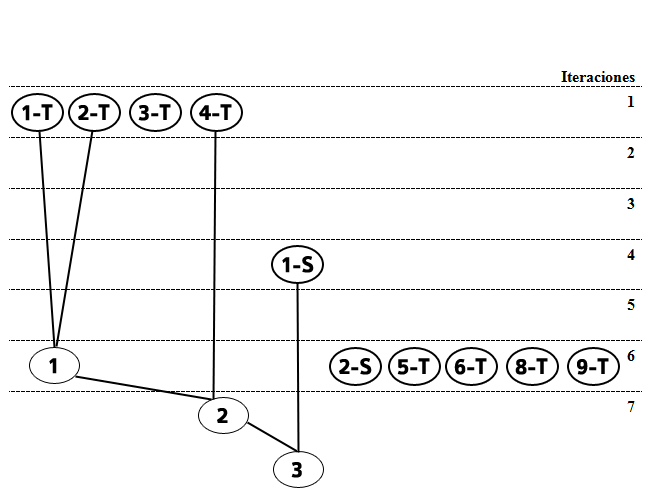
\includegraphics[width=\linewidth]{grafico-seleccion-uos}
	\caption{Progreso del proyecto según selección de UOs}
	\label{fig:grafico-seleccion-uos}
\end{figure}

Los UOs directos aparecen con un borde negro grueso y los UOs por Fusión con un borde negro simple. Las líneas que unen los UOs indican una relación de fusión.\\

\subsection{Desarrollo de modelos por iteraciones}
\label{dgp:desarrollo-actividades}

En la figura ~\ref{fig:grafico-desarrollo-actividades} se detalla el desarrollo de los diferentes tipos de actividad (de desarrollo o de integración) para cada UO en base a las iteraciones.

\begin{figure}[!htbp]
	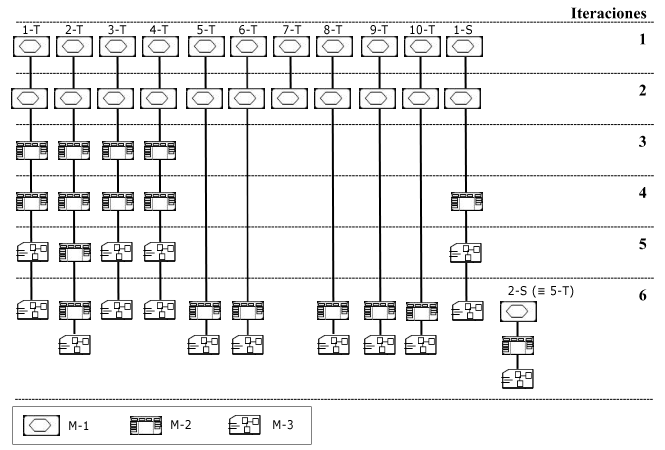
\includegraphics[width=\linewidth]{grafico-desarrollo-actividades}
	\caption{Progreso del proyecto según el desarrollo de Actividades}
	\label{fig:grafico-desarrollo-actividades}
\end{figure}

Las actividades se unen por líneas si estan relacionadas entre sí, estén o no en la misma iteración. Las líneas gruesas indican el flujo normal de desarrollo y las líneas delgadas el flujo de integración.\\

En la iteración final se integraron varios UOs para formar 3 UOs:
\begin{itemize}
\item UO1: UO1-T + UO2-T.
\item UO2: UO1 + UO4-T.
\item UO1: UO2 + UO1-S.
\end{itemize}

%\subsection{Modelos evaluados por iteraciones}
%\label{dgp:modelos-evaluados}

%En la tabla \ref{table:tablas-progreso-modelos-evaluados} se pueden ver valores asociados a cada %par de UO y modelo, estos valores siguen la notación:\\

%\framebox{\parbox[c]{1.0\textwidth}{
%Modelos obtenidos debido a una actividad o proceso:
%\begin{itemize}
%\item X: debido a una DA.
%\item I: debido a una IA.
%\item \underline{I}: debido a una Integración Incremental \underline{IA}.
%\item D: derivado de un proceso de división de un UO.
%\item F: derivado de un proceso de fusión de UOs.
%\end{itemize}
%El número expresa la iteración en la que se evaluó
%satisfactoriamente dicho modelo.
%}}\\

%\noindent
%\begin{table}[h]
%\centering
%\begin{tabu}[h]{|c|[2pt]c|c|c|c|c|c|c|c|c|c|c|c|c|c|}
%  \cline{2-15}
%  \multicolumn{1}{c|}{} & 1-S & 2-S & 1-T & 2-T & 3-T & 4-T & 5-T & 6-T & 8-T & 9-T & 10-T & 1 & %2 & 3\\
%  \cline{1-1} \tabucline[2pt]{2-15}
%  M-1 & X2 & X2 & X2 & X2 & X2 & X2 & X2 & X2 & X2 & X2 & X2 & I6 & I6 & I6\\ 
%  \hline
%  M-2 & X4 & X6 & X4 & X4 & X4 & X4 & X6 & X6 & X6 & X6 & X6 & I6 & I6 & I6\\
%  \hline
%  M-3 & X6 & X6 & X6 & X6 & X6 & X6 & X6 & X6 & X6 & X6 & X6 & I6 &I6 & I6\\
%  \hline
%\end{tabu}
%\caption{Progreso del proyecto según modelos evaluados}
%\label{table:tablas-progreso-modelos-evaluados}
%\end{table}

%\subsection{Hoja de gestión: planificación y UOs}
%\label{dgp:hoja-de-gestion}

%\subsubsection{Planificación (Steps 1.i y 2.i)}
%\label{dgp:hoja-de-gestion:a}

%\noindent
%\begin{tabu}[h]{| l | c | c | c | c | c | c |}
%  \hline                       
%  Iteraciones & 1 & 2 & 3 & 4 & 5 & 6 \\
%  \tabucline[2pt]{1-7} 
%  Lista de UOs & \specialcell{1-T\\2-T\\3-T\\4-T} & & & 1-S & & \specialcell{2-S\\5-T\\6-T\\8-T\%%\9-T\\10-T}\\
%  \tabucline[2pt]{1-7}
%  1º equipo & \specialcell{DA-1(1T)\\DA-1(2T)\\DA-1(3T)\\DA-1(4T)\\DA-1(5T)\\DA-1(6T)\\DA-1(7T)\%%\DA-1(8T)\\DA-1(9T)\\DA-1(10T)} & \specialcell{DA-2(1T)\\DA-2(2T)\\DA-2(3T)\\DA-2(4T)} &  & %DA-2(1S) & \specialcell{DA-3(1S)\\DA-3(1T)\\DA-3(2T)\\DA-3(3T)\\DA-3(4T)} & \specialcell{DA-2(2S)%\\DA-3(2S)\\DA-3(5T)\\DA-3(6T)\\DA-3(8T)\\DA-3(9T)\\DA-3(10T)}\\
%  \hline  
%  2º equipo &  &  &  &  &  & \specialcell{\textbf{Evaluación}\\UO3}  \\
%  \hline  
%  3º equipo & \specialcell{\textbf{Evaluación}\\DA-1(1T)\\DA-1(2T)\\DA-1(3T)\\DA-1(4T)\\DA-1(5T)\%\DA-1(6T)\\DA-1(7T)\\DA-1(8T)\\DA-1(9T)\\DA-1(10T)} &  &  & \specialcell{\textbf{Evaluación}\%\DA-2(1T)\\DA-2(2T)\\DA-2(3T)\\DA-2(4T)} &  & \specialcell{\textbf{Evaluación}\\UO3} \\
%  \hline  
%  4º equipo &  &  &  &  &  &  \\
%  \hline 
%\end{tabu}
%\captionof{table}{Planificación (Steps 1.i y 2.i)}
%\label{dgp:hoja-de-gestion:a:tabla}

%----------------------------------------------------%
%     				 SEGUIMIENTO                     %
%----------------------------------------------------%

\section{Seguimiento}
\label{seguimiento}

La dedicación total al proyecto ha sido de 264 horas y 56 minutos horas. Al acabar la iteración 6 se habían dedicado 223 horas y 56 minutos.\\

\subsubsection{Dedicación por tipo de tarea}
\label{seguimiento:tipo-tarea}

\begin{figure}[!htbp]
	\centering
	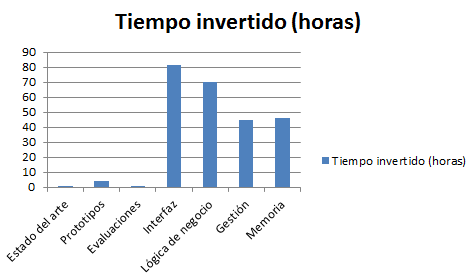
\includegraphics[height=6cm, keepaspectratio]{seguimiento}
	\caption{Dedicación por tipo de tarea}
	\label{fig:seguimiento}
\end{figure}

\subsubsection{Dedicación del progreso por meses}
\label{seguimiento:tiempo}

\begin{figure}[!htbp]
	\centering
	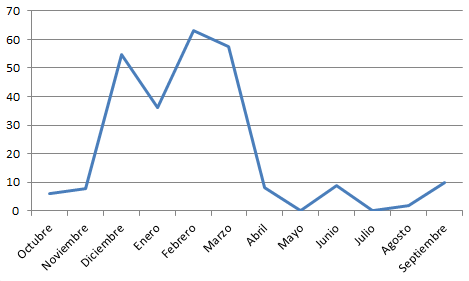
\includegraphics[height=6cm, keepaspectratio]{seguimiento-2}
	\caption{Dedicación por meses}
	\label{fig:seguimiento-2}
\end{figure}

%----------------------------------------------------%
%              ANALISIS DE REQUISITOS                %
%----------------------------------------------------%

%----------------------------------------------------%
%              ANALISIS DE REQUISITOS                %
%----------------------------------------------------%

\chapter{Análisis de Requisitos}
\label{analisis-de-requisitos}

Este apartado contiene dos secciones mayores: el apartado \ref{analisis-de-requisitos:no-funcionales} en el que se detallan los requisitos no-funcionales y el apartado \ref{analisis-de-requisitos:funcionales} en el que se explican los requisitos funcionales recogidos de los modelos M-1 de cada UO.\\

\section{Requisitos no-funcionales}
\label{analisis-de-requisitos:no-funcionales}

La aplicación ha sido desarrollada con dos requisitos básicos:

\begin{itemize}
\item Que tenga mucha funcionalidad con el mínimo posible de \textit{clicks}.
\item Que para el alumno no suponga una distracción.
\end{itemize}

Asi pues se ha creado un diseño agradable que pretende tener mucha funcionalidad, especialmente en la vista de profesor. En la vista del alumno se ha minimizado el diseño y los elementos para que no existan distracciones importantes en clase.\\

\subsection{Requisitos de la interfaz}
\label{analisis-de-requisitos:no-funcionales:interfaz}

Para hacer más intuitiva la aplicación se han concretado unos colores e iconos específicos para cada tipo de ejercicio, de modo que sea fácil asociar una acción o estado mediante un color o un icono.

\begin{itemize}
\item Ejercicios activos: color rojo, pretendiendo indicar actividad, y un icono de un avión de papel, simbolizando un ejercicio que ha sido lanzado.
\item Ejercicios finalizados: color azul, indicando calma (ya hemos terminado), y un icono de una bandera de meta, simbolizando el fin.
\item Ejercicios preparados: color amarillo y un icono de un reloj, indicando que esto no se ha lanzado aun (viendo las aplicaciones móvil más utilizadas resulta intuitivo el significado del reloj).
\end{itemize}

Para las estadísticas se ha dejado el color verde y un icono de un gráfico de barras. El color azul se emplea para otros botones, sin usar ningún icono.\\

\section{Requisitos funcionales}
\label{analisis-de-requisitos:funcionales}

En este apartado se presentan los requisitos funcionales recogidos en interfaces de papel

Siguiendo las pautas fijadas por los requisitos no-funcionales se han realizado interfaces sencillas e intuitivas. Se le ha dado mucha importancia a la filosofía de ''en pocos \textit{clicks}'' que sigue la aplicación. Por tanto, ante todo, se han minimizado la cantidad de transiciones entre pantallas y el uso de excesivos botones para buscar mucha funcionalidad en pocos \textit{clicks}.\\

El resultado queda plasmado en estos modelos de requisitos (M-1) de cada objetivo de usuario (\textit{User Objective}). Los modelos están construidos mediante diferentes pantallas, las comunes al estudiante y al profesor son nombradas PX, donde X es el número de la pantalla, y las que son exclusivas de cada uno se denotan como \[PX_{Y}\]donde X es el número de la pantalla e Y es el usuario (puede tomar los valores S para el estudiante y T para el profesor).\\

\subsection{Requisito común: Autenticación}
\label{analisis-de-requisitos:funcionales:p1}

La autenticación es un requisito común para todos los UOs. En las figuras \ref{fig:autenticacion-alumno} y \ref{fig:autenticacion-profesor} se ve el autómata de estados correspondiente a la autenticación de un alumno y la de un profesor, respectivamente. Ambos autómatas comparten algunas pantallas, llamadas P0\textsubscript{I} y P0\textsubscript{II}, que se engloban en P0.\\

\noindent
\begin{figure}[!htbp]
\noindent
\makebox[\textwidth][c]{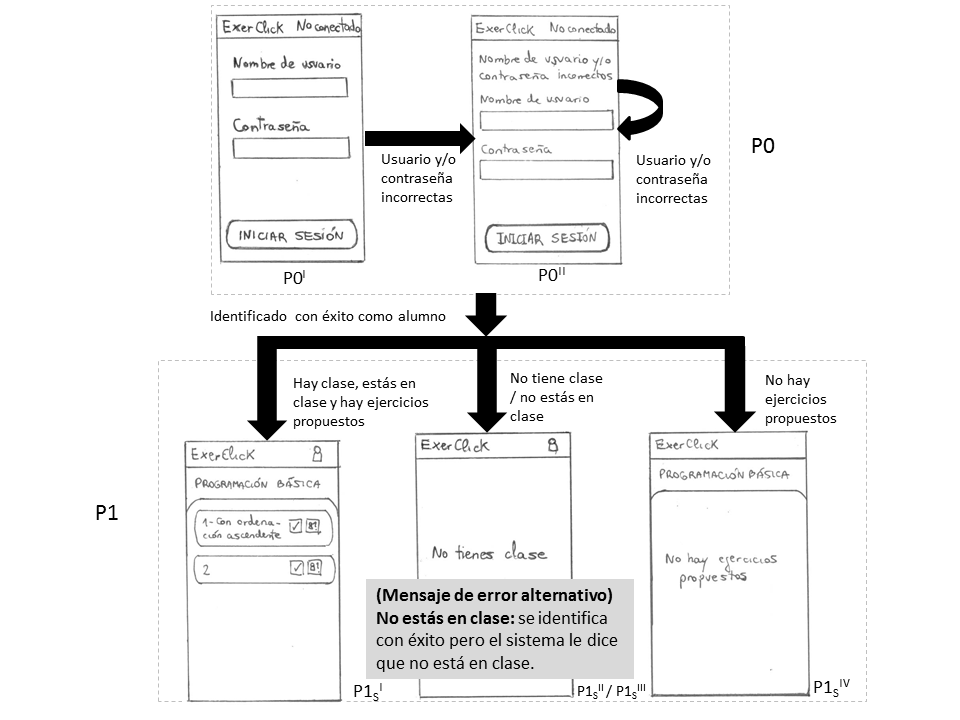
\includegraphics[width=\textwidth,keepaspectratio]{fsm2/autenticacion-s}}
\caption{Autómata de estados correspondiente a la autenticación del alumno}
\label{fig:autenticacion-alumno}
\end{figure}

\noindent
\begin{figure}[!htbp]
\noindent
\makebox[\textwidth][c]{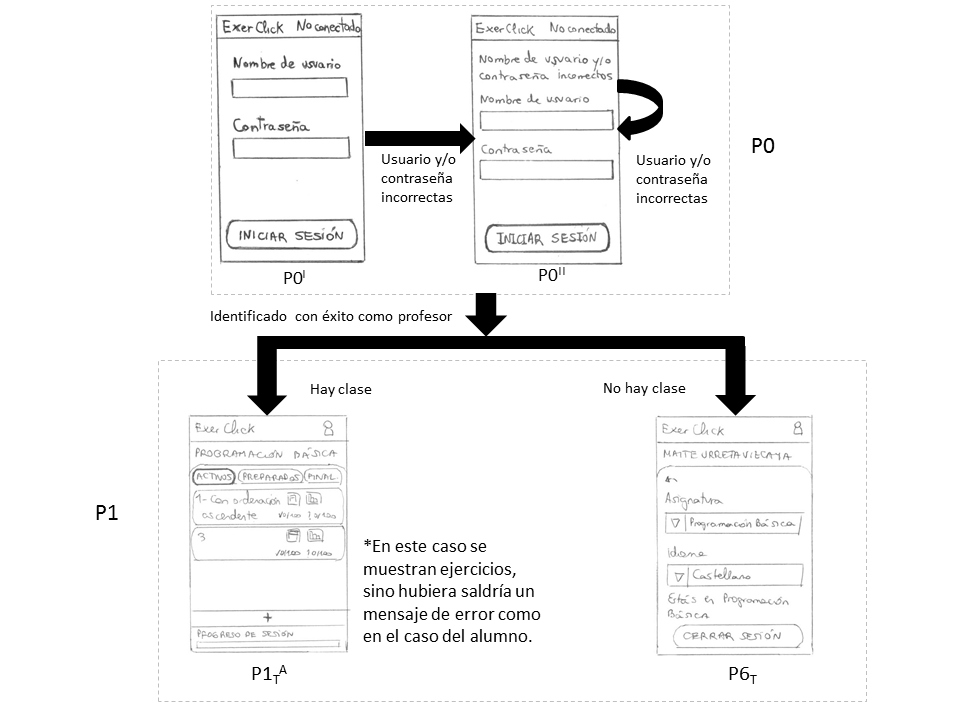
\includegraphics[width=\textwidth,keepaspectratio]{fsm2/autenticacion-t}}
\caption{Autómata de estados correspondiente a la autenticación del profesor}
\label{fig:autenticacion-profesor}
\end{figure}

En cualquier variante de P0 podemos ver dos campos para introducir nuestro nombre de usuario y contraseña y un botón para acceder. Si los datos son correctos (y tenemos clase\footnote{Se considera que hay clase desde la hora de inicio de la clase hasta la hora final y también durante 15 minutos antes de la hora de inicio}, además de estar en ella\footnote{Para reconocer que un alumno ha entrado en clase este tiene que fichar con su tarjeta de alumno.}) veremos la interfaz P1 del profesor o del estudiante (dependiendo del tipo de usuario con el que no hayamos autenticado, P1\textsubscript{S}\textsuperscript{I} para el alumno y P1\textsubscript{T}\textsuperscript{A} para el profesor). Si los datos introducidos son incorrectos iremos a P0\textsubscript{I}. También podemos ver variantes de P1 en el caso del alumno si no tenemos clase, no estamos en clase o no hay ejercicios propuestos.\\

Durante este capítulo se asumirá que el usuario se ha autenticado correctamente (como alumno o como profesor) y está en su correspondiente pantalla principal. Por tanto se obviará que todos los UOs deben pasar por P0 antes de llegar a sus pantallas iniciales.\\

\subsection{UO1-S: Responder a un ejercicio}
\label{analisis-de-requisitos:funcionales:uo1s}

El modelo M-1(1-S) requiere de la pantalla principal del alumno (P1\textsubscript{S}) Como se comentó en el apartado anterior se da por hecho que el alumno se identificó correctamente, tiene clase, está en ella y hay ejercicios propuestos. En P1\textsubscript{S} podemos responder a los ejercicios indefinidamente "sin cambiar de pantalla". No nos iremos a otra pantalla, sino que esta variará. Esta transición se puede apreciar en la figura \ref{fig:analisis-de-requisitos:funcionales:uo1s}.\\

\noindent
\begin{figure}[!htbp]
\noindent
\makebox[\textwidth][c]{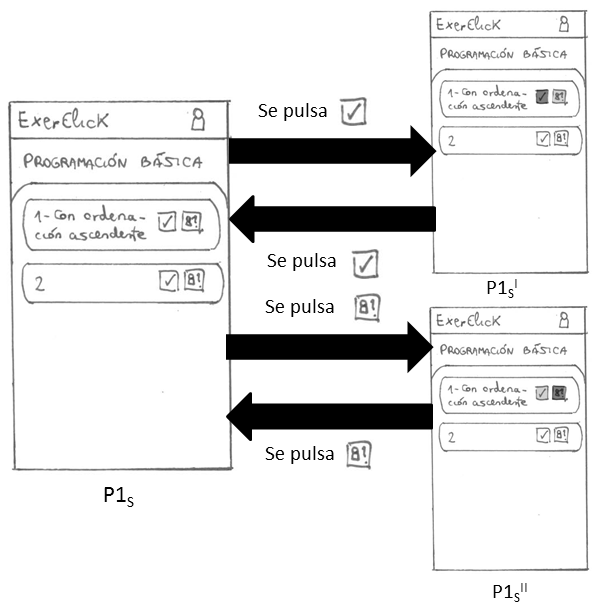
\includegraphics[width=0.7\textwidth,keepaspectratio]{fsm2/uo1s}}
\caption{Autómata de estados correspondiente al UO1-S}
\label{fig:analisis-de-requisitos:funcionales:uo1s}
\end{figure}

Nuestras opciones para responder a un ejercicio son marcar el ejercicio como finalizado (este botón será azul) o marcar una duda en el ejercicio (este será rojo). En la figura \ref{fig:analisis-de-requisitos:funcionales:uo1s} se puede ver en la parte de arriba el proceso de marcar un ejercicio como finalizado y de desmarcarlo. Análogamente para marcarlo con una duda en la parte de abajo de la misma figura.\\

\subsection{UO2-S: Ver la descripción completa de un ejercicio}
\label{analisis-de-requisitos:funcionales:uo2s}

El modelo M-1(2-S) cuenta con una pantalla P2\textsubscript{S} a la que se accede mediante P1\textsubscript{S}. En la figura \ref{fig:analisis-de-requisitos:funcionales:uo2s} se puede ver el autómata de estados correspondiente. Haciendo \textit{click} sobre el contenedor de cualquier ejercicio (sobre la ''caja'') podremos acceder a P2\textsubscript{S}. La interfaz se carga con datos sobre el ejercicio sobre el que hemos hecho \textit{click} (identificador siempre y opcionalmente cualquier otro dato que el profesor haya incluido). Si no hubiera más detalles añadidos aparecerá un mensaje avisando de ello. En P2\textsubscript{S} se aprecia un enlace ''+Más'' que estaba pensado para mostrar más detalles sobre el ejercicio. Este enlace es eliminado de aquí en adelante.\\

\noindent
\begin{figure}[!htbp]
\noindent
\makebox[\textwidth][c]{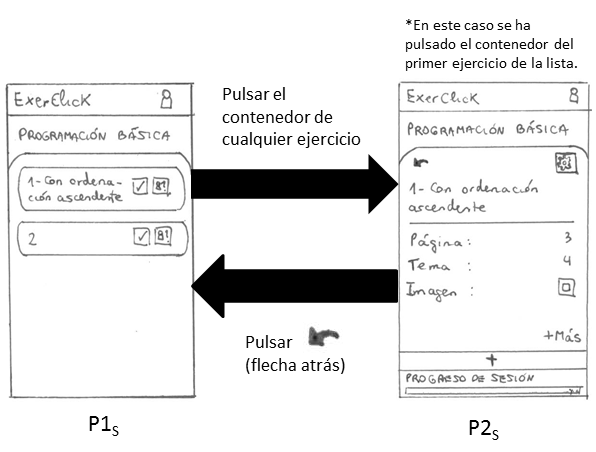
\includegraphics[width=\textwidth,keepaspectratio]{fsm2/uo2s}}
\caption{Autómata de estados correspondiente al UO2-S}
\label{fig:analisis-de-requisitos:funcionales:uo2s}
\end{figure}

\subsection{UO1-T + UO2-T: Crear-Lanzar un ejercicio simple/detallado}
\label{analisis-de-requisitos:funcionales:uo1t}

En esta sección se comentarán los UOs 1-T y 2-T, ya que el UO2-T es un modelo incremental del UO1-T, y, por tanto, están estrechamente ligados. Se comenzará hablando del UO1-T y más adelante del UO2-T.\\

\subsubsection{UO1-T: P2\textsubscript{T} (primer modelo)}

Estando en el sistema autenticados y con acceso a la asignatura, podemos crear-lanzar ejercicios pulsando en el símbolo '+', que nos da acceso a la pantalla nueva P2\textsubscript{T}, accesible desde cualquier variante de P1. En la primera versión de P2\textsubscript{T} (figura \ref{fig:analisis-de-requisitos:funcionales:uo1t:p2-viejo}) había 4 campos básicos para crear un ejercicio: un identificador, la página, el tema y una imagen. Todos los campos menos el identificador eran opcionales. Sin embargo, más tarde se pensó en reducir esto para que se viera más simple.\\

\begin{figure}[!htbp]
	\centering
	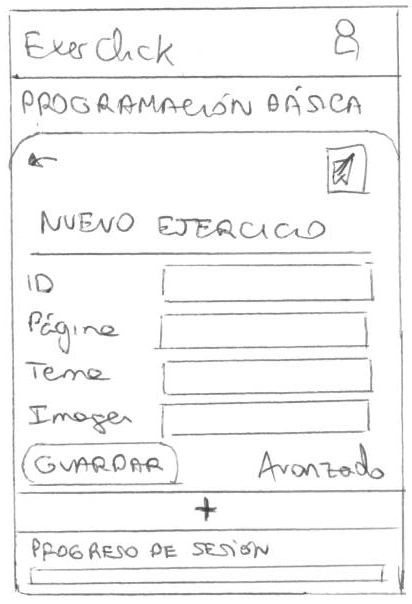
\includegraphics[height=7cm]{sheetprotos/teacher/p2-old}
	\caption{P2: Crear-Lanzar un ejercicio simple (primer modelo)}
	\label{fig:analisis-de-requisitos:funcionales:uo1t:p2-viejo}
\end{figure}

Tenemos dos botones disponibles: el de la parte superior (con un avión de papel) que lanzará directamente el ejercicio como un ejercicio activo y el de la parte inferior que guardará el ejercicio como ejercicio preparado para que podamos seguir editándolo antes de lanzarlo. Para guardar o lanzar un ejercicio es necesario que el campo del identificador no esté vacío. La flecha hacia atrás cerrará la interfaz y volveremos a P1\textsubscript{T}. Finalmente, disponemos de un enlace ''Avanzado'' que nos llevará a la interfaz P2\textsubscript{T}\textsuperscript{I}.\\

\subsubsection{UO1-T: P2\textsubscript{T} (nuevo modelo)}

En la nueva versión de la interfaz P2\textsubscript{T} (figura \ref{fig:analisis-de-requisitos:funcionales:uo1t:p2}) se utiliza la interfaz de P1, añadiendo por encima una pestaña nueva en la que podremos crear un ejercicio simple. Estos ejercicios sólo necesitan de un identificador, por tanto, en esta pequeña pestaña sólo hay un campo para añadir ese identificador. Los campos omitidos pueden ser añadidos mediante el UO2-T (en la pantalla P2\textsubscript{T}\textsuperscript{I}). Además se añade la opción de cerrar la ventana haciendo \textit{click} fuera de ésta. El enlace en el que antes ponía ''Más'' ahora por ''Avanzado'', pero en cuanto a funcionalidad sigue siendo lo mismo (muestra mas detalles para personalizar el ejercicio). Precisamente, mostrar más detalles es el objetivo del UO2-T.\\

\begin{figure}[!htbp]
	\centering
	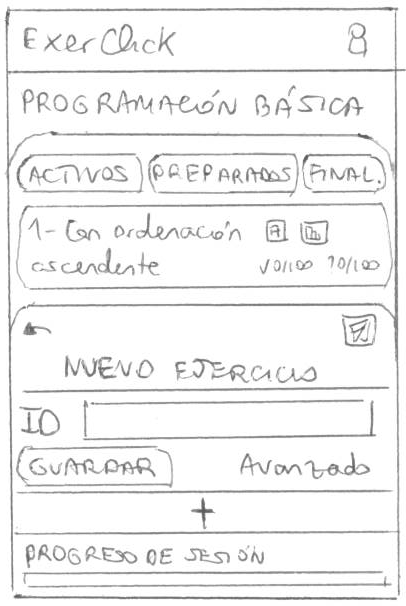
\includegraphics[height=7cm]{sheetprotos/teacher/p2}
	\caption{P2: Crear-Lanzar un ejercicio simple}
	\label{fig:analisis-de-requisitos:funcionales:uo1t:p2}
\end{figure}

\subsubsection{UO2-T}

Desde P2\textsubscript{T} es posible acceder a P2\textsubscript{T}\textsuperscript{I} pulsando sobre el enlace ''Avanzado'' (como se ha comentado previamente). Esta pantalla tiene un gran parecido con el primer modelo de P2\textsubscript{T}. Añade varios campos extra (página y tema) respecto a la nueva versión de P2\textsubscript{T}. La flecha hacia atrás cierra por completo la ventana superpuesta sobre P1\textsubscript{T}. Nuevamente el enlace ''Más'' se elimina más adelante. En la figura \ref{fig:analisis-de-requisitos:funcionales:uo1+2t:fsm} se ve el autómata de estados completo que fusiona los UOs 1-T y 2-T.\\

\noindent
\begin{figure}[!htbp]
\noindent
\makebox[\textwidth][c]{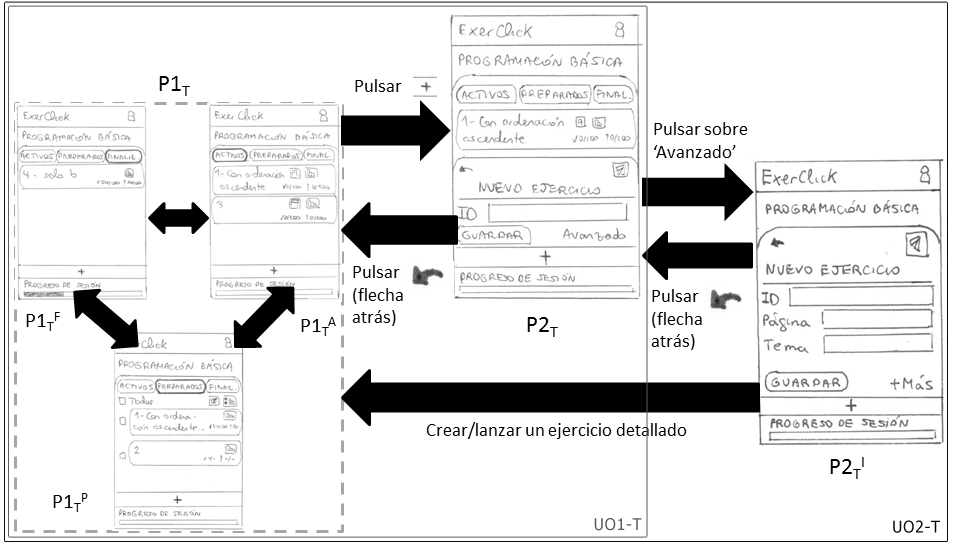
\includegraphics[width=\textwidth,keepaspectratio]{fsm2/uo1+2t}}
\caption{Autómata de estados correspondiente a los UOs 1-T y 2-T}
\label{fig:analisis-de-requisitos:funcionales:uo1+2t:fsm}
\end{figure}

\subsection{UO3-T: Cambiar el tipo de ejercicio}
\label{analisis-de-requisitos:funcionales:uo3t}

Este UO al principio tenía como finalidad cambiar un ejercicio de activo a finalizado (es decir, dar por finalizado un ejercicio propuesto en clase). Se cambió a "cambiar el tipo de un ejercicio" para dar más libertad y poder enmendar errores (ya que se daba la posibilidad de cambiar de cualquier tipo a otro). En los prototipos en papel no aparecen todos los botones, sólo la versión vieja (con el botón para finalizar ejercicios nada más).\\

Se deciden usar 3 iconos (figura \ref{fig:analisis-de-requisitos:funcionales:uo3t:iconos}) para representar cada tipo de ejercicio para que resulten intuitivos sin usar texto.\\

\begin{figure}[!htbp]
\centering
\begin{subfigure}[t]{0.3\textwidth}
	\centering
	
\includegraphics{avion-papel}
	\caption{Ejercicios activos}
	\label{fig:analisis-de-requisitos:funcionales:uo3t:iconos-1}
\end{subfigure}
%
\centering
\begin{subfigure}[t]{0.3\textwidth}
	\centering
	
\includegraphics{bandera-meta}
	\caption{Ejercicios finalizados}
	\label{fig:analisis-de-requisitos:funcionales:uo3t:iconos-2}
\end{subfigure}
%
\centering
\begin{subfigure}[t]{0.3\textwidth}
	\centering
	
\includegraphics{reloj}
	\caption{Ejercicios preparados}
	\label{fig:analisis-de-requisitos:funcionales:uo3t:iconos-3}
\end{subfigure}

\caption{Iconos utilizados para representar cada tipo de ejercicio}
\label{fig:analisis-de-requisitos:funcionales:uo3t:iconos}
\end{figure}

Desde cualquiera de las variantes de P1: P1\textsubscript{T}\textsuperscript{A} (ejercicios activos), P1\textsubscript{T}\textsuperscript{F} (ejercicios finalizados) y P1\textsubscript{T}\textsuperscript{P} (ejercicios propuestos) podemos hacer cambios. En la figura \ref{fig:analisis-de-requisitos:funcionales:uo3t:fsm} se puede ver el autómata de estados por el que se guían estos cambios.\\

\noindent
\begin{figure}[!htbp]
\noindent
\makebox[\textwidth][c]{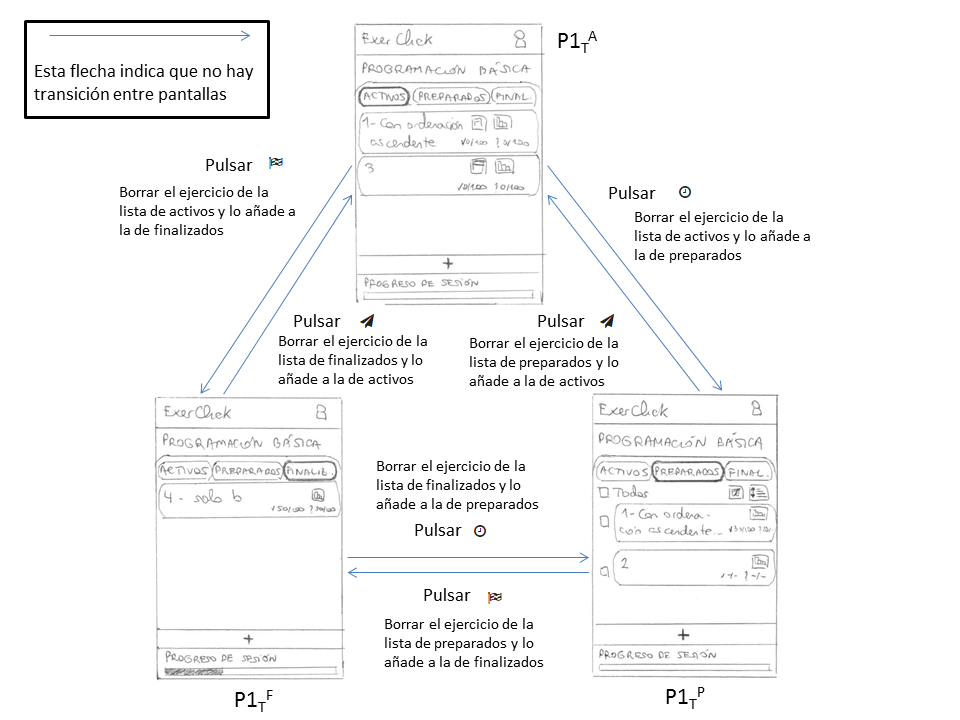
\includegraphics[width=\textwidth,keepaspectratio]{fsm2/uo3t}}
\caption{Autómata de estados correspondiente al UO3-T}
\label{fig:analisis-de-requisitos:funcionales:uo3t:fsm}
\end{figure}

Finalmente, existe una limitación a estos cambios para un caso especial. Cuando el profesor entra en la aplicación (puede hacerlo en cualquier momento, aunque no haya clase, tal y como se ve en la figura \ref{fig:autenticacion-profesor}) y quiere lanzar un ejercicio. Un requisito especial es que los ejercicios sólo pueden ser lanzados en clase. Es decir, si el profesor accede a la aplicación y no hay clase no puede crear ejercicios directamente para lanzar (UO1-T/UO2-T) ni cambiar un ejercicio al tipo activo.\\

\subsection{UO4-T: Ver estadísticas de un ejercicio}
\label{analisis-de-requisitos:funcionales:uo4t}

El profesor puede ver las estadísticas de un ejercicio, siempre y cuando sea un ejercicio activo o finalizado. Las estadísticas se muestran en tres pantallas diferentes: P2\textsubscript{T}\textsuperscript{T}, P5\textsubscript{T}\textsuperscript{A} y P5\textsubscript{T}\textsuperscript{D}.

\begin{itemize}
\item \textbf{P5\textsubscript{T}\textsuperscript{T}:} nos muestra a todos los alumnos involucrados en el ejercicios (que estén en la asignatura) en forma de lista. Muestra, por cada alumno, el estado de realización del ejercicio: acabado, con alguna duda o sin marcar nada.\\

Tanto P5\textsubscript{T}\textsuperscript{A} como P5\textsubscript{T}\textsuperscript{D} son filtros aplicados a la lista de P5\textsubscript{T}\textsuperscript{T}.
\item \textbf{P5\textsubscript{T}\textsuperscript{A}:} nos filtra sólo los alumnos que han marcado el ejercicio como acabado.
\item \textbf{P5\textsubscript{T}\textsuperscript{D}:} igual que P5A pero marcando como duda el ejercicio.
\end{itemize}

En la figura \ref{fig:analisis-de-requisitos:funcionales:uo4t:fsm} podemos ver el autómata de estados correspondiente al UO4-T.\\

\noindent
\begin{figure}[!htbp]
\noindent
\makebox[\textwidth][c]{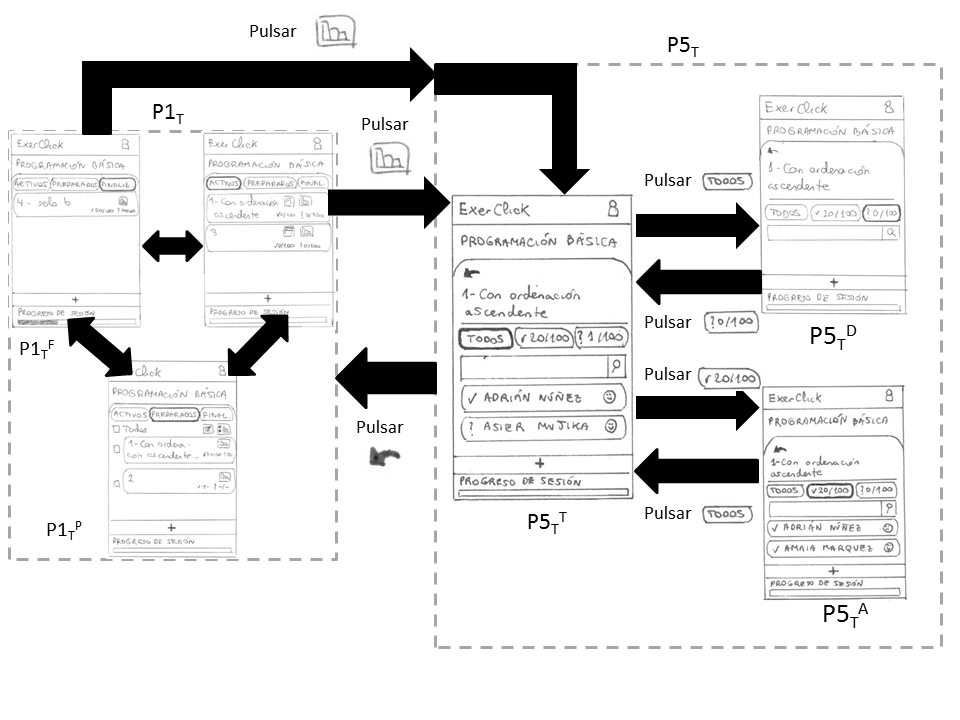
\includegraphics[width=\textwidth,keepaspectratio]{fsm2/uo4t}}
\caption{Autómata de estados correspondiente al UO4-T}
\label{fig:analisis-de-requisitos:funcionales:uo4t:fsm}
\end{figure}

Desde P1\textsubscript{T}\textsuperscript{A} o P1\textsubscript{T}\textsuperscript{F} siempre accederemos directamente a P5\textsubscript{T}\textsuperscript{T} y desde ésta podemos acceder a P5\textsubscript{T}\textsuperscript{A} y P5\textsubscript{T}\textsuperscript{D} mediante la pulsación de los botones de la parte superior. En los botones de finalizados y duda aparecen iconos, el número de acabados/dudas respecto al número de alumnos en formato n/m y el mismo dato en formato de porcentaje.\\

\subsection{UO5-T + UO6-T: Ver la descripción completa y editar un ejercicio}
\label{analisis-de-requisitos:funcionales:uo5t}

En este apartado detallaremos el análisis de requisitos de los UOs 5-T y 6-T. El UO6-T es un modelo incremental del UO5-T (al igual que los UOs 1-T y 2-T).\\

\subsubsection{UO5-T}

Es posible ver la descripción completa de un ejercicio (UO5T) desde cualquier variante de P1 (P1\textsubscript{T}\textsuperscript{A}, P1\textsubscript{T}\textsuperscript{F} o P1\textsubscript{T}\textsuperscript{P}), haciendo \textit{click} sobre el contenedor de cualquier ejercicio (sobre la ''caja'') podremos acceder a P3, tal y como se muestra en la figura \ref{fig:analisis-de-requisitos:funcionales:uo5t:fsm}. La interfaz se carga con datos sobre el ejercicio sobre el que hemos hecho \textit{click} (identificador siempre y opcionalmente cualquier otro dato que hayamos introducido como profesor). Si no hubiera más detalles añadidos aparecerá un mensaje avisando de ello.\\

Este UO es similar al UO2-S del alumno. Sin embargo, a diferencia del UO2-S (donde se mostraban también los detalles de un ejercicio) en P3 tenemos un botón con un engranaje en la parte superior, al pulsarlo nos llevará a P4 (editar el ejercicio). El enlace ''+Más'' sigue igual que en el UO2-S, sirve para mostrar más detalles. Más tarde es eliminado.\\

\noindent
\begin{figure}[!htbp]
\noindent
\makebox[\textwidth][c]{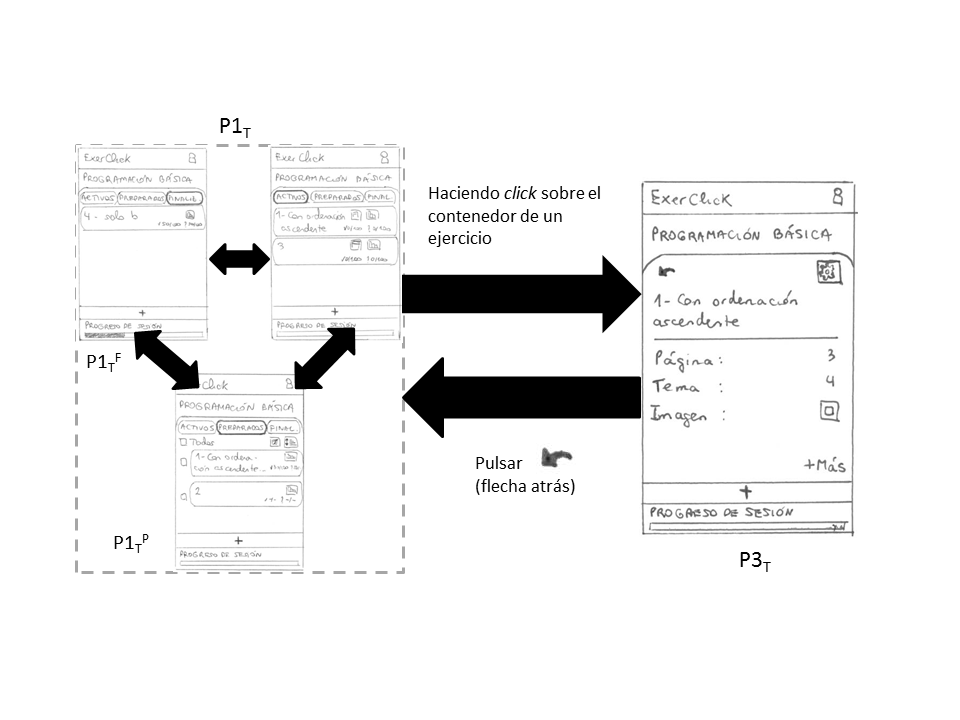
\includegraphics[width=\textwidth,keepaspectratio]{fsm2/uo5t}}
\caption{Autómata de estados correspondiente al UO5-T}
\label{fig:analisis-de-requisitos:funcionales:uo5t:fsm}
\end{figure}

\subsubsection{UO6-T}

Accederemos a P4\textsubscript{T} mediante P3\textsubscript{T} utilizando el botón con un engranaje (figura \ref{fig:analisis-de-requisitos:funcionales:uo6t:fsm}). En esta nueva pantalla podremos editar el ejercicio del que estábamos viendo los detalles en P3\textsubscript{T}.\\

En la nueva ventana tenemos el título del ejercicio y la flecha de ir atrás como en P3. En el centro de la ventana tenemos un campo por cada detalle del ejercicio, el campo se cargará con el valor previo (si tuviese). Podemos editar esos valores y pulsar el botón de ''Guardar'' para que se guarden los cambios. Si pulsamos atrás los cambios no se guardarán.\\

Más adelante el botón de atrás se elimina y se mantiene el botón de engranaje, pulsar este botón tiene el mismo efecto que la flecha para ir hacia atrás. También se cambia el título de la ventana (donde sale el título del ejercicio) por un campo con el título del ejercicio. Este campo es editable, lo cual permite editar el identificador del ejercicio (este campo no se puede dejar vacío).\\

El enlace ''Más'' muestra más detalles que editar (aunque fue eliminado más adelante).\\

\noindent
\begin{figure}[!htbp]
\noindent
\makebox[\textwidth][c]{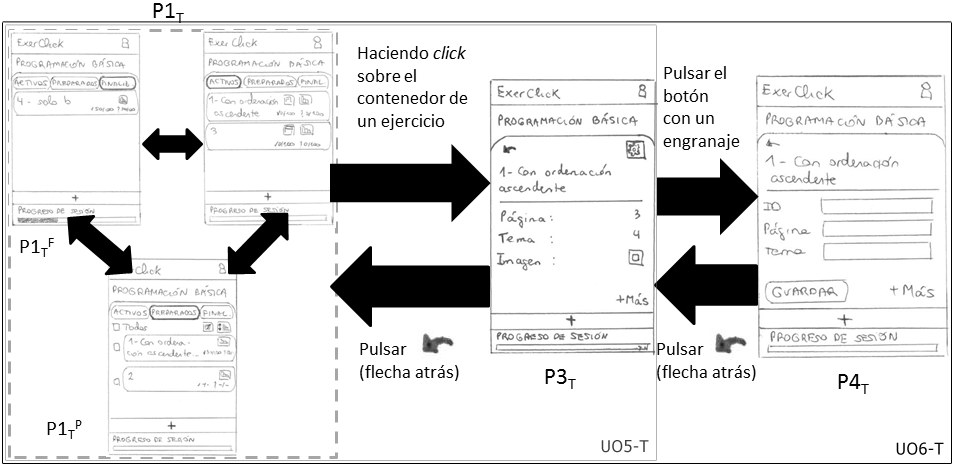
\includegraphics[width=\textwidth,keepaspectratio]{fsm2/uo6t}}
\caption{Autómata de estados correspondiente a los UOs 5-T y 6-T}
\label{fig:analisis-de-requisitos:funcionales:uo6t:fsm}
\end{figure}

\subsection{UO8-T + UO9-T + UO10-T: Cerrar sesión, Cambiar el idioma y la asignatura de la aplicación}
\label{analisis-de-requisitos:funcionales:uo8t}

La última interfaz de la aplicación es P6\textsubscript{T}. Esta interfaz es el perfil del profesor, donde se pueden realizar algunas opciones:
\begin{itemize}
\item \textbf{UO8-T:} Cerrar la sesión abierta (y volver a la pantalla inicial, P0).
\item \textbf{UO9-T:} Cambiar el idioma de la aplicación (entre Castellano, Euskera, Inglés y Francés).
\item \textbf{UO10-T:} Cambiar la asignatura activa.
\end{itemize}

Para acceder al perfil hay que hacer \textit{click} sobre el nombre de usuario o el símbolo de usuario de la parte superior derecha de la aplicación. La pantalla del perfil tiene dos desplegables (para escoger idioma y para escoger asignatura), un campo para mostrar la asignatura activa (de la que se muestran ejercicios en P1\textsubscript{T}) y un botón para cerrar sesión. Más tarde en lugar de la flecha hacia atrás que hay en la parte superior se pone un botón con el texto ''Ir a clase'' para volver a P1\textsubscript{T} (es decir, el mismo efecto que la flecha hacia atrás). En el perfil podremos realizar las acciones descritas previamente de la siguiente forma:

\begin{itemize}
\item \textbf{Cerrar sesión:} Tenemos que pulsar el botón ''Cerrar sesión'' de la parte inferior. Volveremos a P0, y desde ahí podemos autenticarnos de nuevo.
\item \textbf{Cambiar de idioma:} En el perfil del profesor aparecerá una opción ''Idioma'' con un desplegable. Al escoger cualquier opción de este la aplicación cambiará automáticamente de idioma (no hay transición de pantallas).
\item \textbf{Cambiar de asignatura:} Existe otra opción con desplegable llamada ''Asignatura'', donde podemos escoger entre cualquier asignatura del profesor. Al escoger una nueva asignatura no se apreciarán más cambios que el texto que aparece sobre el botón de cerrar sesión (donde aparece la asignatura que está seleccionada), sin embargo la ''asignatura activa'' ha cambiado. Es decir, si volvemos de nuevo a los ejercicios (P1\textsubscript{T}) veremos que estamos en la nueva asignatura seleccionada, y, por tanto, aparecerán los ejercicios de esa asignatura.\\
\end{itemize}

Todo se resume en el autómata de estados de la figura \ref{fig:analisis-de-requisitos:funcionales:uo8-9-10t:fsm}, donde aparecen las transiciones de los 3 UOs.\\

\noindent
\begin{figure}[!htbp]
\noindent
\makebox[\textwidth][c]{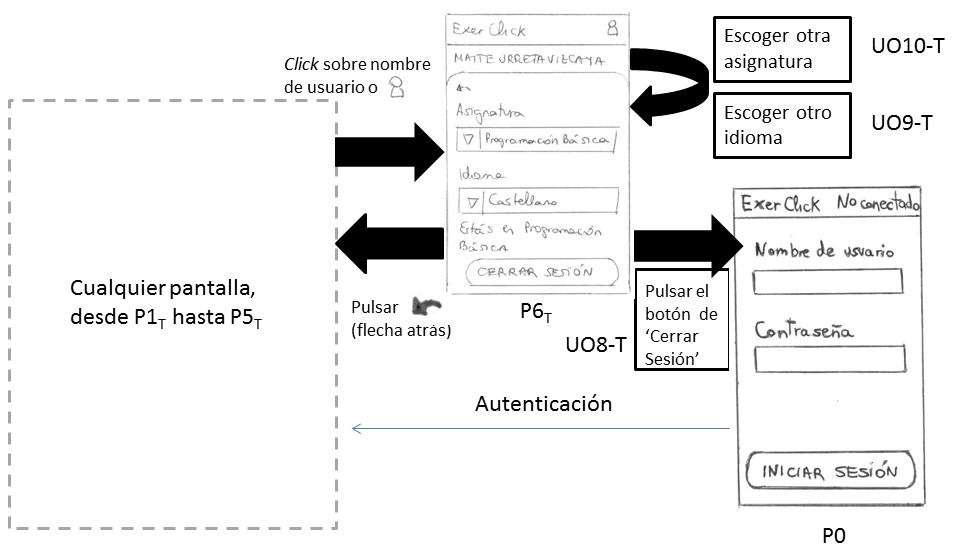
\includegraphics[width=\textwidth,keepaspectratio]{fsm2/uo8-9-10t}}
\caption{Autómata de estados correspondiente a los UOs 8-T, 9-T y 10-T}
\label{fig:analisis-de-requisitos:funcionales:uo8-9-10t:fsm}
\end{figure}

%\subsection{UO1: Lanzar ejercicios}
%\label{analisis-de-requisitos:funcionales:uo1}

%\noindent
%\begin{figure}[!htbp]
%\noindent
%\makebox[\textwidth][c]{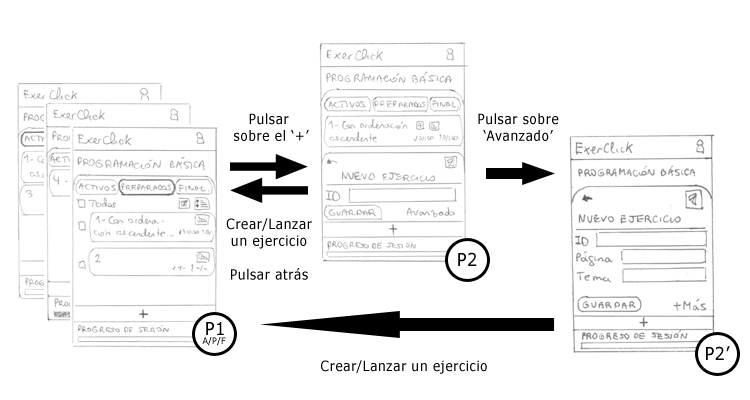
\includegraphics[width=\textwidth,keepaspectratio]{fsm2/uo1}}
%\caption{Autómata de estados correspondiente al UO1}
%\label{fig:analisis-de-requisitos:funcionales:uo1:fsm}
%\end{figure}

%Este modelo es una combinación de los UO1-T (Crear-lanzar un ejercicio simple) y UO2-T (Crear-lanzar un ejercicio %avanzado), permite crear un ejercicio simple o uno avanzado (dependiendo de las necesidades del profesor).\\

%\subsection{UO2: Lanzar ejercicios y visualizar resultados}
%\label{analisis-de-requisitos:funcionales:uo2}

%\noindent
%\begin{figure}[!htbp]
%\noindent
%\makebox[\textwidth][c]{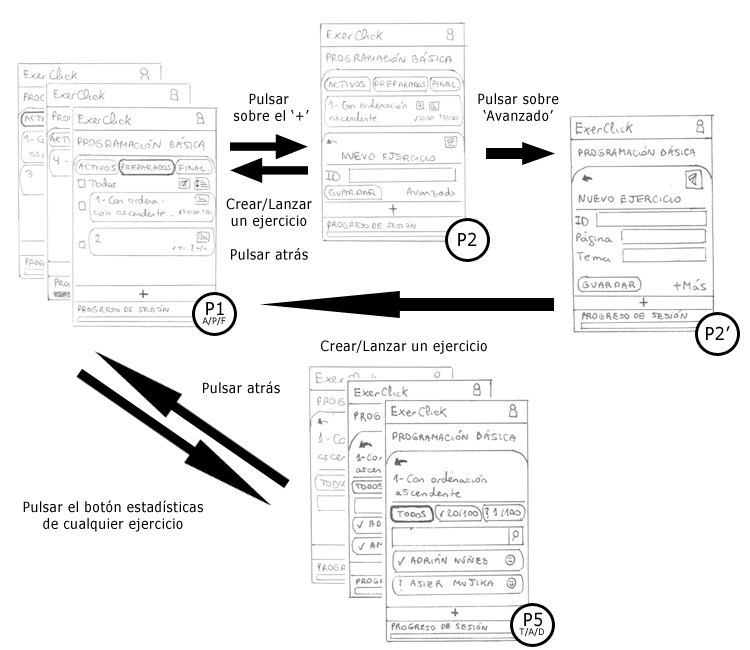
\includegraphics[width=\textwidth,keepaspectratio]{fsm2/uo2}}
%\caption{Autómata de estados correspondiente al UO2}
%\label{fig:analisis-de-requisitos:funcionales:uo2:fsm}
%\end{figure}

%Combinando el UO1 anterior con el UO4-T (ver estadísticas de un ejercicio) obtenemos el UO2 de la figura %\ref{fig:analisis-de-requisitos:funcionales:uo2:fsm}.\\

%----------------------------------------------------%
%              DISEÑO E IMPLEMENTACIÓN               %
%----------------------------------------------------%

%----------------------------------------------------%
%              DISEÑO E IMPLEMENTACIÓN               %
%----------------------------------------------------%

\chapter{Diseño e Implementación}
\label{diseno-e-implementacion}

En este capítulo tenemos dos apartados importantes: el \ref{diseno-e-implementacion:interfaces} en el que se muestran las interfaces y, en general, el lado cliente y el \ref{diseno-e-implementacion:logica-negocio} en el que se muestra la lógica de negocio. Al final del capítulo se detalla la estructura de ficheros y carpetas del proyecto en el apartado \ref{diseno-e-implementacion:estructura} y los requisitos para ejecutar la aplicación en el apartado \ref{diseno-e-implementacion:dispositivos}.\\

\section{M-2: Interfaces o lado del cliente}
\label{diseno-e-implementacion:interfaces}

En este apartado se mostrarán las interfaces desarrolladas partiendo de los modelos de requisitos (M-1) de cada objetivo y algunos elementos comunes de todos los objetivos.

\subsection{Interfaz de autenticación de usuario}
\label{diseno-e-implementacion:interfaces:autenticacion}

A modo de ejemplo se añade el prototipo en papel correspondiente a esta pantalla (figura ~\ref{fig:autenticacion:diseno}) para que se aprecie la diferencia de estilo.\\

La pantalla de autenticación de usuario (index.html) de la figura ~\ref{fig:autenticacion:diseno} es la primera que se muestra al iniciar la aplicación. Esta pantalla nos redirige a teacher.html o student.html (vista del profesor y del alumno, respectivamente) dependiendo del rol del usuario con el que nos identifiquemos (el rol está definido en la base de datos).\\

\noindent
\begin{figure}[!htbp]
\begin{subfigure}[t]{0.5\textwidth}
	\centering
	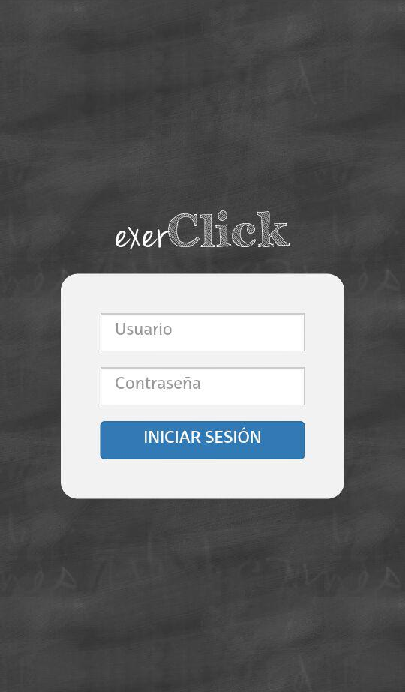
\includegraphics[height=7cm, frame]{autenticacion}
	\caption{Diseño (M-2)}
    \label{fig:autenticacion:diseno}
\end{subfigure}
%
\begin{subfigure}[t]{0.5\textwidth}
	\centering
	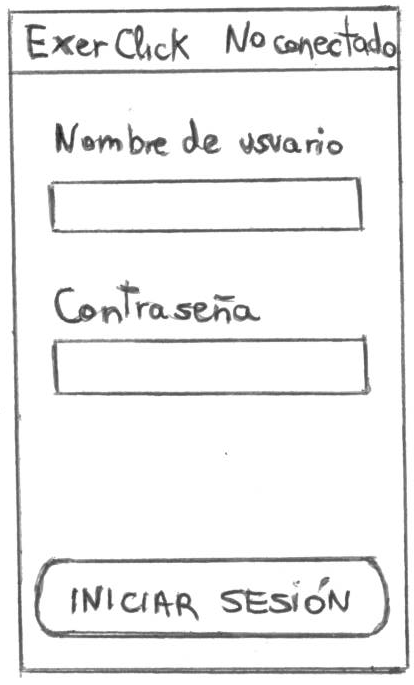
\includegraphics[height=7cm, frame]{sheetprotos/p0}
	\caption{Prototipo en papel (M-1)}
	\label{fig:autenticacion:proto}
\end{subfigure}
%
\caption{Pantalla de autenticación de usuario}
\label{fig:autenticacion}
\end{figure}

\textbf{\textit{qClick}} \cite{qclick} y \textbf{\textit{exerClick}} comparten la misma base de datos y el sistema de autenticación de ambos es similar. Por ello, se decidió utilizar el mismo sistema de autenticación de qClick en exerClick y se reutilizó la mayor parte del código.\\

\subsection{Interfaz del alumno}
\label{diseno-e-implementacion:interfaces:alumno}

La pantalla del alumno (figura \ref{diseno-e-implementacion:interfaces:alumno}) le muestra a este el estado actual de la clase: los ejercicios activos, su progreso en esta sesión y la media de progreso de la clase.

\noindent
\begin{figure}[!htbp]
\begin{subfigure}[t]{0.3\textwidth}
	\centering
	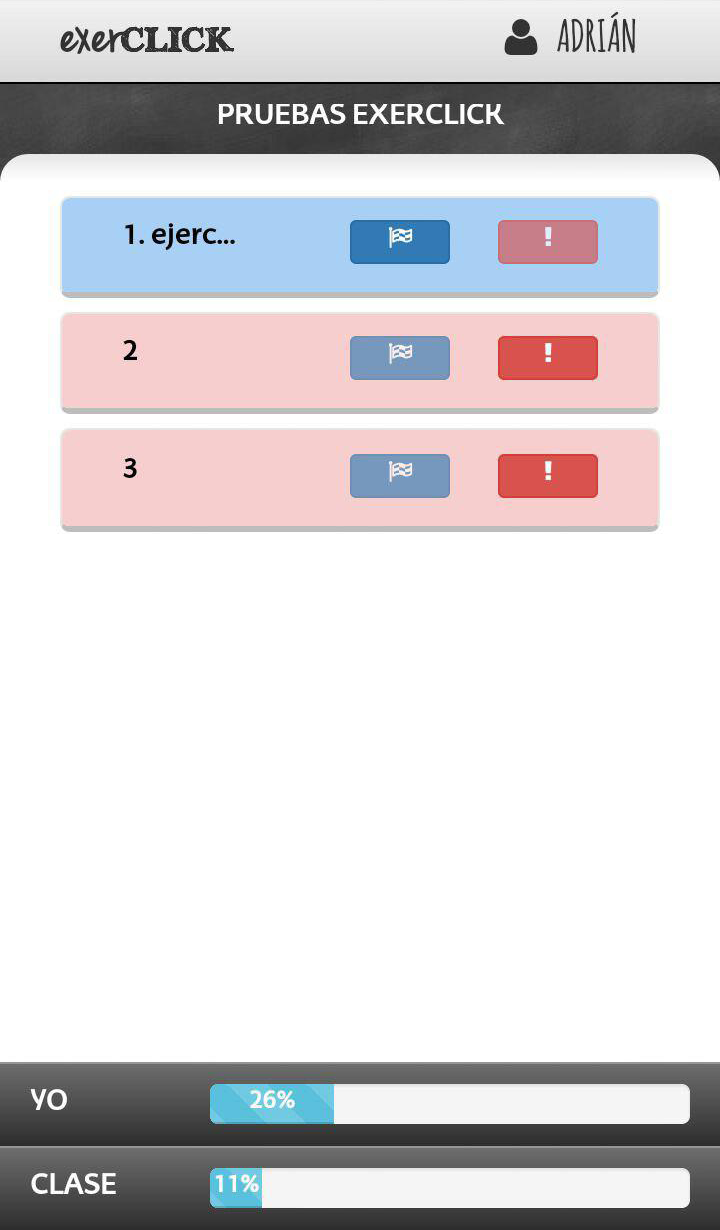
\includegraphics[height=5cm, frame]{P1-S}
	\caption{P1\textsubscript{S}: versión móvil}
	\label{fig:diseno-e-implementacion:interfaces:alumno:p1}
\end{subfigure}
%
\begin{subfigure}[t]{0.7\textwidth}
	\centering
	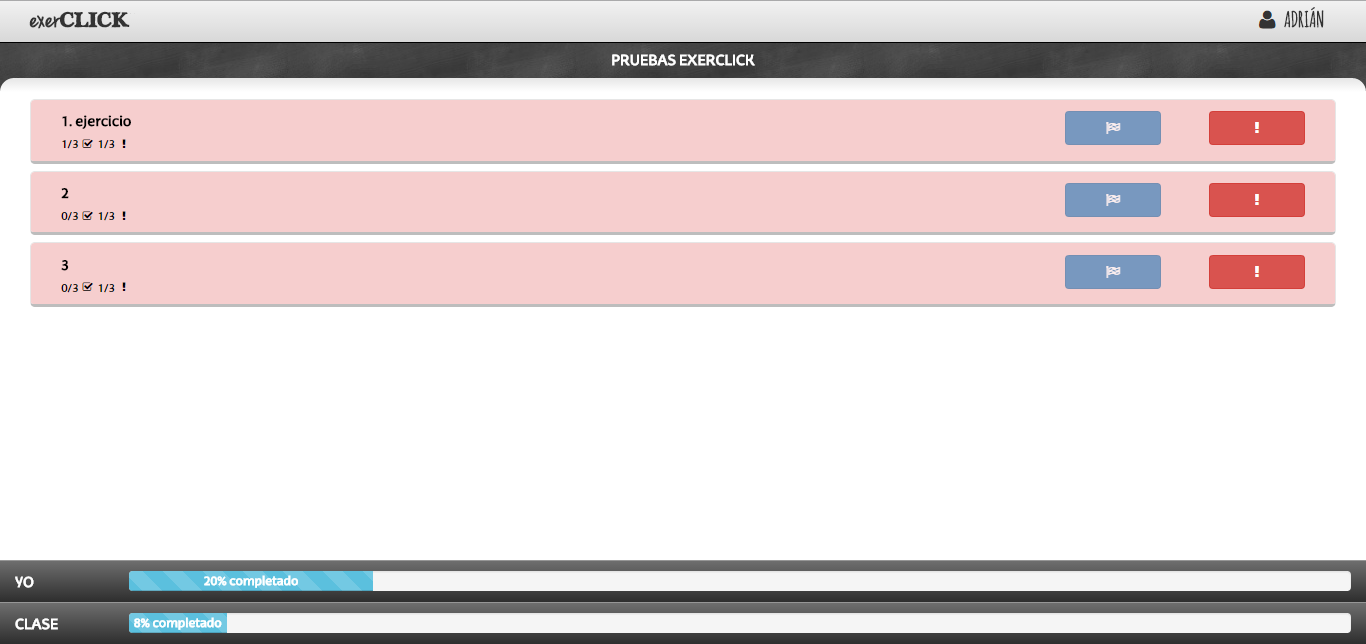
\includegraphics[height=5cm, frame]{P1-S_big}
	\caption{P1\textsubscript{S}: versión tableta}
	\label{fig:diseno-e-implementacion:interfaces:alumno:p1_big}
\end{subfigure}

\caption{P1\textsubscript{S}: vista del alumno}
\label{diseno-e-implementacion:interfaces:alumno}
\end{figure}

\subsubsection{UO1-S: Responder a un ejercicio}
\label{diseno-e-implementacion:interfaces:alumno:uo1-s}

En la figura \ref{fig:p1-student} se muestra la pantalla principal del alumno, (P1\textsubscript{S}). En la barra superior aparece el nombre de usuario e inmediatamente debajo el nombre de la asignatura de la que hay una sesión activa.\\

Las cajas son ejercicios activos en esa asignatura. Para que el estado de los ejercicios sea más visible las cajas tienen colores: el rojo es para una duda y el azul para un ejercicio acabado. Dentro de las cajas aparece el nombre de los ejercicios a la izquierda y a la derecha dos botones para marcar el estado en el que nos encontramos con cada ejercicio.\\

\noindent
\begin{figure}[!htbp]
\begin{subfigure}[t]{0.5\textwidth}
	\centering
	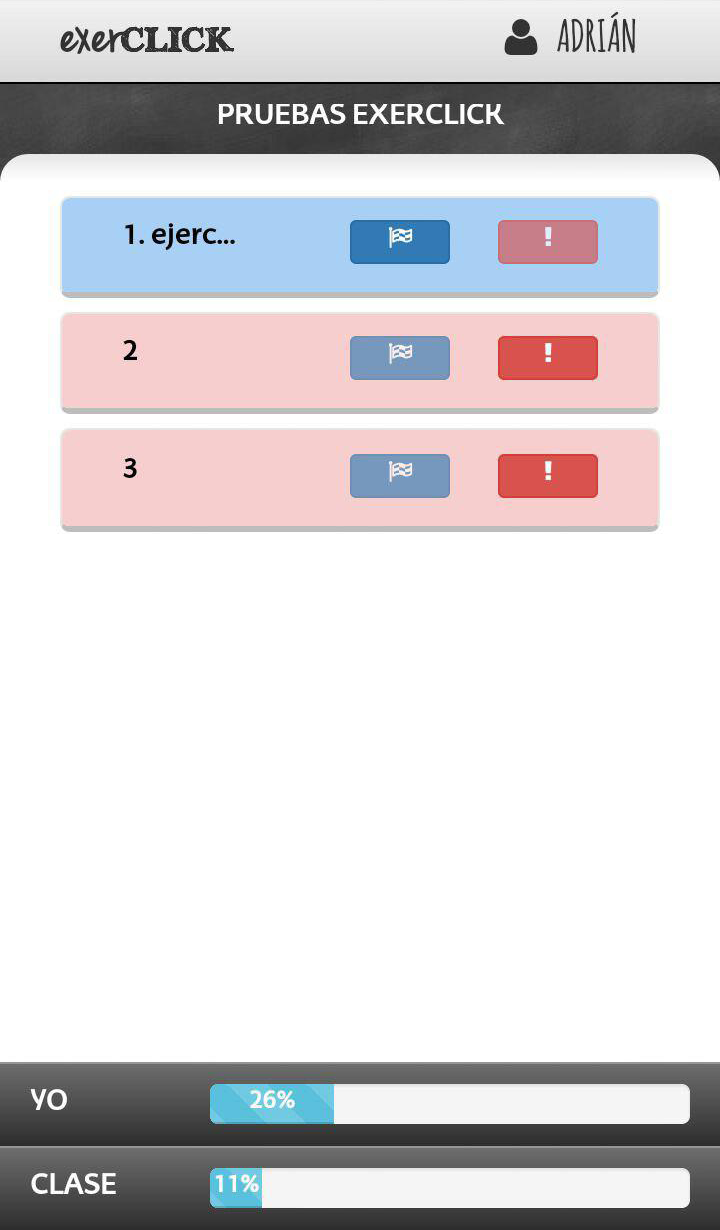
\includegraphics[height=7cm, frame]{P1-S}
	\caption{P1\textsubscript{S}: vista principal, se muestran los ejercicios}
	\label{fig:diseno-e-implementacion:interfaces:alumno:p1}
\end{subfigure}
%
\begin{subfigure}[t]{0.5\textwidth}
	\centering
	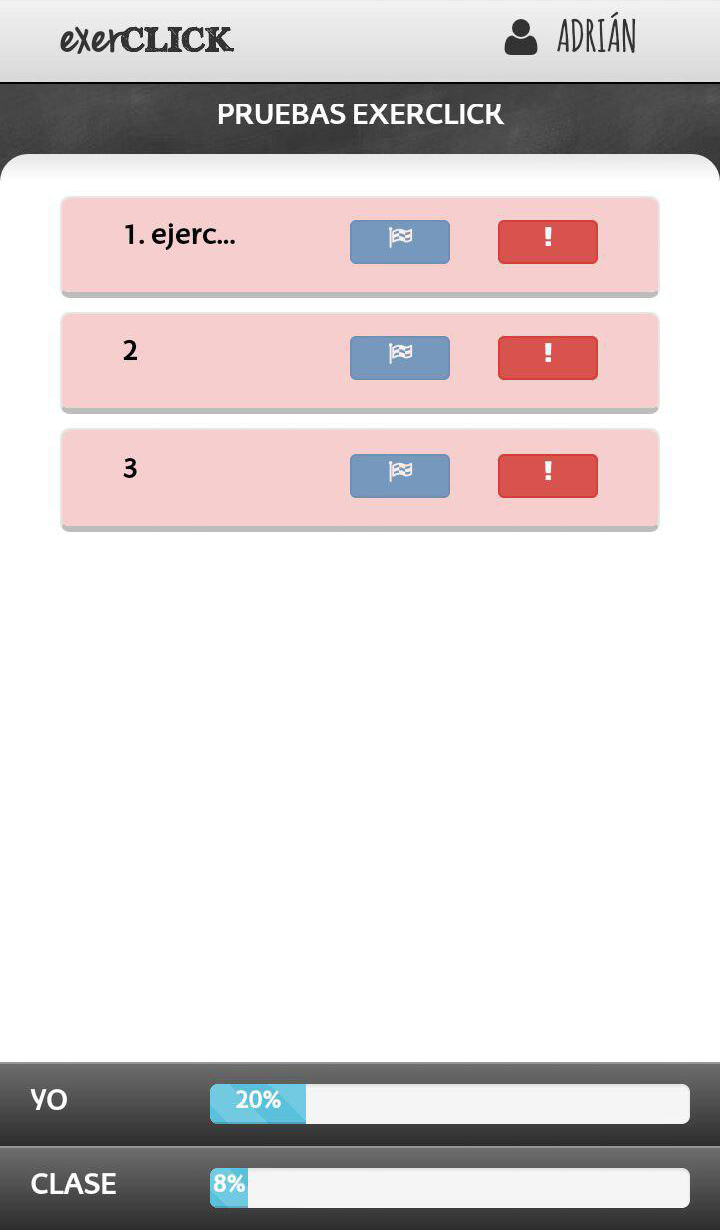
\includegraphics[height=7cm, frame]{P1-S'}
	\caption{P1\textsubscript{S}: cambio en el estado de un ejercicio}
	\label{fig:diseno-e-implementacion:interfaces:alumno:p1'}
\end{subfigure}

\caption{P1\textsubscript{S}: cambio en el estado de un ejercicio}
\label{fig:p1-student}
\end{figure}

En la figura \ref{fig:diseno-e-implementacion:interfaces:alumno:p1} cada uno de los ejercicios tiene un estado (finalizado o con duda) denotado por el botón que está activado (el otro al estar desactivado tiene menos opacidad). También se puede apreciar en el color del contenedor del ejercicio, si está en azul es que está marcado como finalizado (botón azul también iluminado y rojo apagado) y análogamente si el contenedor es rojo.\\

Para cambiar el estado de un ejercicio (UO1-T) debemos darle al botón activado/iluminado (es decir, quitar la marca que habíamos hecho) para que el ejercicio se quede sin estado (nada marcado, la caja toma un color gris). Cuando la caja está gris ambos botones están iluminados y podemos, por tanto, marcar un nuevo estado (el que queramos). Se puede ver parte de la transición en la figura \ref{fig:p1-student}: el ejercicio ''1º ejercicio'' está marcado como acabado y en la figura \ref{fig:diseno-e-implementacion:interfaces:alumno:p1'} está marcado como duda al igual que el resto (habiendo estado sin marca previamente).\\

\subsubsection{UO2-S: Ver detalles de un ejercicio}
\label{diseno-e-implementacion:interfaces:alumno:uo2-s}

Al pulsar sobre un ejercicio podremos ver la pantalla P2 del alumno. Los detalles del ejercicio sobre el que hemos pinchado se cargan en una pestaña, tal y como se ve en la figura \ref{diseno-e-implementacion:interfaces:alumno:p2}. Tenemos un botón para ir atrás y cerrar la pestaña en la parte superior, junto al identificador del ejercicio. En el cuerpo de la pestaña aparecen los detalles de uno en uno, podemos bajar gracias al \textit{scroll} para ver todos los detalles.\\

Un añadido respecto al M-1 es que P2\textsubscript{S} es una ventana solapada a la interfaz P1\textsubscript{S}, y por tanto se puede hacer \textit{click} fuera de ella. Al hacerlo se cerrará automáticamente la ventana. Daremos por hecho de aquí en adelante que cualquier ventana solapada a una interfaz, que tenga un espacio fuera de ella para hacer \textit{click}, puede cerrarse al hacer click fuera de la ventana.\\

\noindent
\begin{figure}[!htbp]
	\centering
	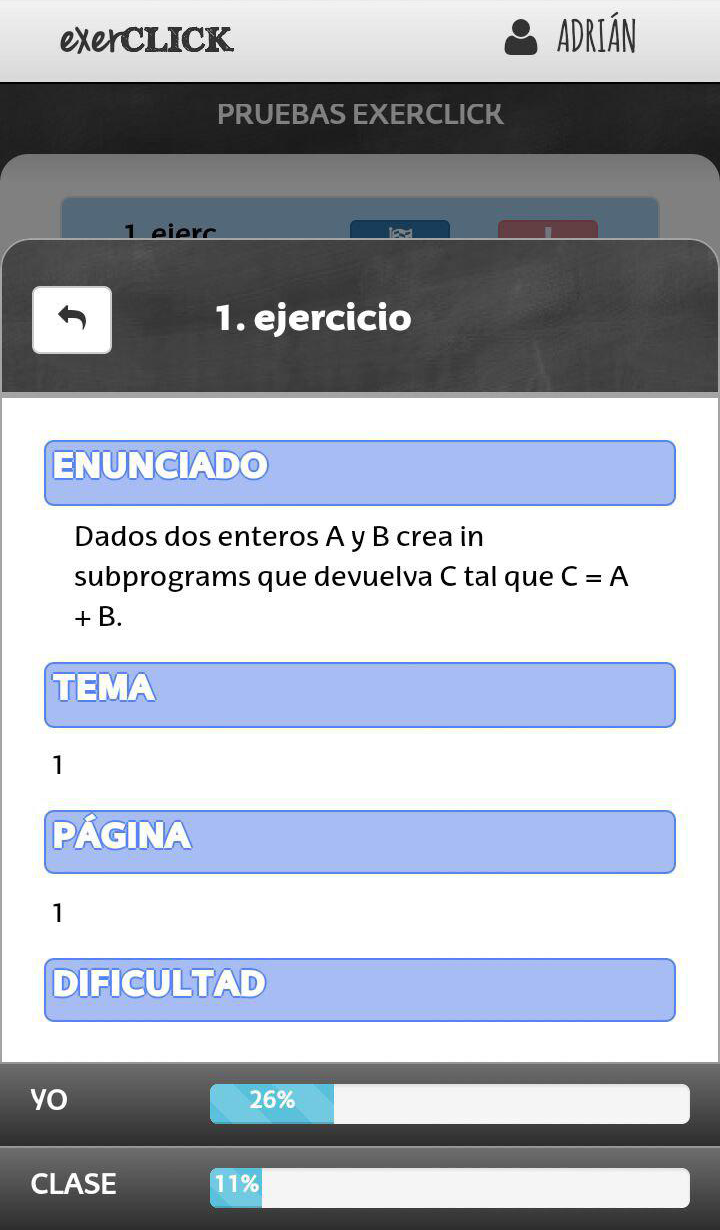
\includegraphics[height=7cm, frame]{P2-S}
	\caption{P2\textsubscript{S}: ver los detalles de un ejercicio}
	\label{diseno-e-implementacion:interfaces:alumno:p2}
\end{figure}

\subsection{Interfaz del profesor}
\label{diseno-e-implementacion:interfaces:profesor}

Cuando nos identificamos como profesor, si hay una clase activa, accederemos directamente a esta pantalla (teacher.html) que aparece en la figura \ref{diseno-e-implementacion:interfaces:profesor}. Además sirve como base de muchos UOs del profesor, ya que hay que pasar obligatoriamente por ella. En ella se muestra en la parte superior el nombre del usuario identificado y justo debajo el nombre de la asignatura activa.\\

\noindent
\begin{figure}[!htbp]
\begin{subfigure}[t]{0.3\textwidth}
	\centering
	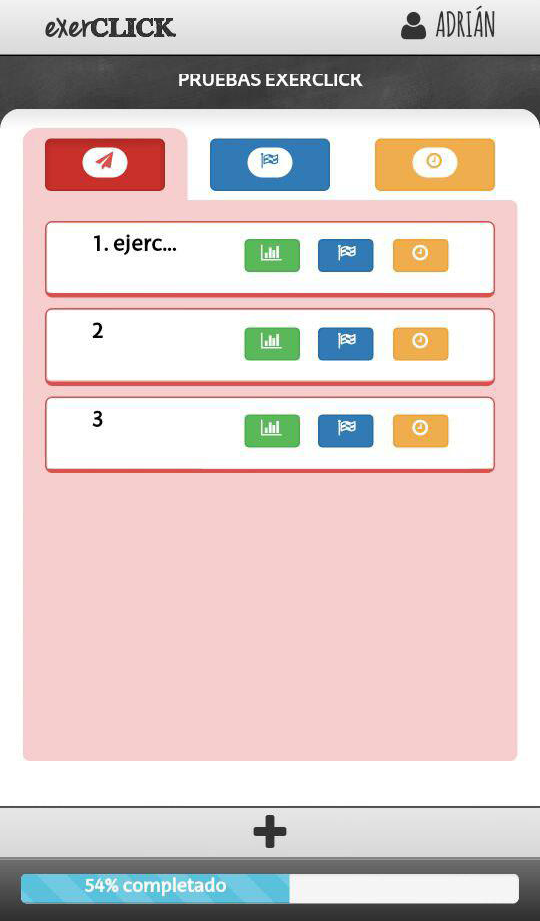
\includegraphics[height=7cm, frame]{activos}
	\caption{P1\textsubscript{T}\textsuperscript{A}: versión móvil}
	\label{fig:activos}
\end{subfigure}
%
\begin{subfigure}[t]{0.7\textwidth}
	\centering
	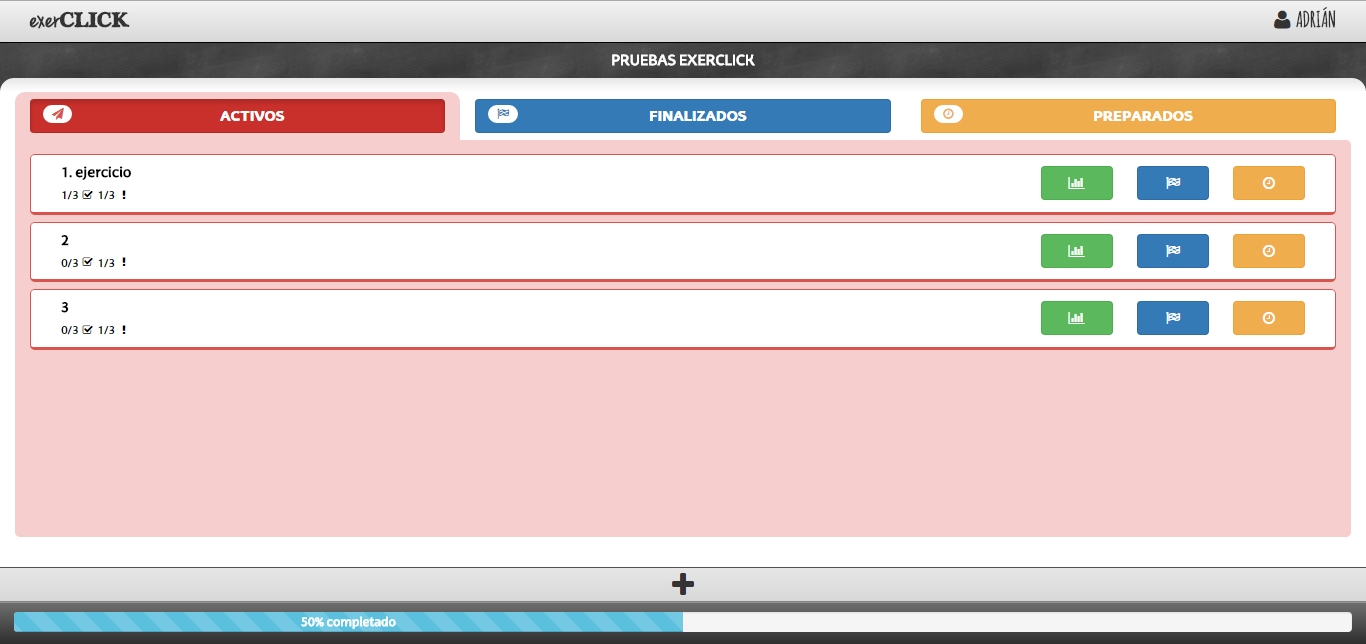
\includegraphics[width=\textwidth, frame]{P1_big}
	\caption{P1\textsubscript{T}\textsuperscript{A}: versión tableta}
	\label{fig:activos_g}
\end{subfigure}

\caption{P1\textsubscript{T}\textsuperscript{A}: Vista del profesor}
\label{diseno-e-implementacion:interfaces:profesor}
\end{figure}

En el centro tenemos tres botones de colores y una lista de ejercicios (si la hubiera). La lista de ejercicios que aparece al cargar esta interfaz por primera vez es la de ejercicios activos propuestos en clase (que los alumnos pueden ver). Estos ejercicios corresponden al botón rojo. Pulsando el botón azul se mostrarán los ejercicios finalizados y pulsando el botón amarillo los preparados (son ejercicios guardados que se quieren lanzar).\\

En cada caja de ejercicios veremos el nombre del ejercicio en la parte izquierda y en la derecha tres botones. El botón verde sirve para mostrar las estadísticas (UO4-T) en la pantalla P5\textsubscript{T} y los otros dos cambian dependiendo del tipo de ejercicios que se muestren. Su función es cambiar el tipo del ejercicio (UO3-T). Así, un ejercicio activo, al pulsar el botón azul se cambiará a finalizado.\\

Finalmente, en la parte de abajo hay dos barras. La primera, con un '+', sirve para mostrar la pestaña para crear ejercicios nuevos (UO1-T, UO2-T y UO1). La barra inferior a esta muestra el progreso en la sesión, es decir: cuántos ejercicios han sido dados por finalizados respecto a los lanzados.\\

\subsection{Interfaz del perfil del profesor}
\label{diseno-e-implementacion:interfaces:perfil}

Es la interfaz de profile.html (figura \ref{fig:perfil}\label{fig:perfil}), y la vista de profesor de inicio después de autenticarse si no hay ninguna sesión activa en marcha (no hay clase). Desde esta pantalla podemos cambiar algunas opciones como la asignatura activa (aparece un mensaje de cuál es la asignatura activa más abajo) o el idioma de la aplicación. El botón de ''Ir a clase'' nos devuelve a la pantalla P1\textsubscript{T} (teacher.html) con la asignatura activa escogida. En la parte inferior hay un botón para cerrar sesión y volver a la pantalla de autenticación (P0).\\

\noindent
\begin{figure}[!htbp]
	\centering
	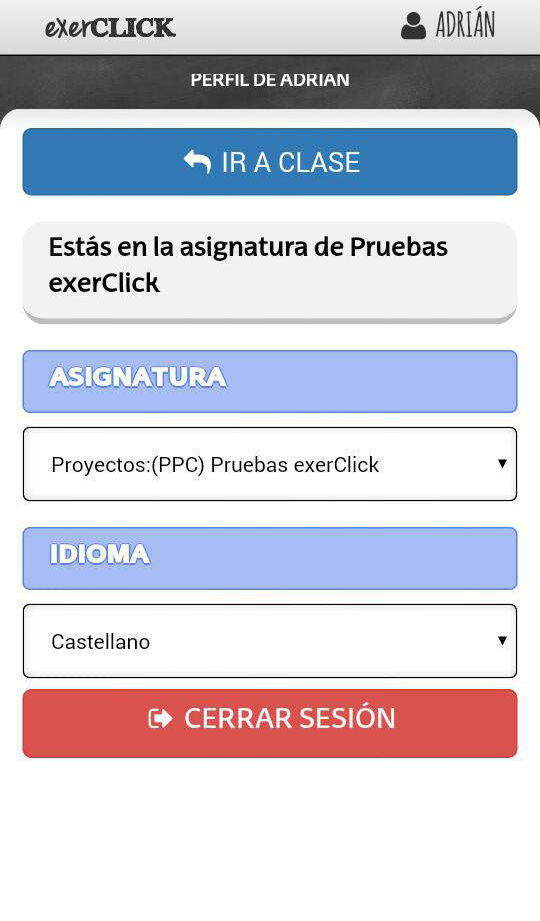
\includegraphics[height=7cm, frame]{perfil}
	\caption{Perfil del profesor}
	\label{fig:perfil}
\end{figure}

\subsubsection{UO1-T: Crear-Lanzar un ejercicio simple}
\label{diseno-e-implementacion:interfaces:profesor:uo1-t}

Al pulsar el botón con símbolo de '+' (\textit{plus}/más) de la parte inferior de la interfaz del profesor se desplegará la pestaña que aparece en la figura ~\ref{fig:crear-lanzar-ejercicio-simple}. En la parte superior tenemos la el botón con una flecha hacia atrás para cerrar la pestaña, el identificador del ejercicio y el botón para lanzar el ejercicio. Este botón sólo estará activo si estamos en clase, de otro modo sólo podremos guardar el ejercicio.\\

En la parte central hay un campo para añadir el identificador del ejercicio (obligatorio). Hay dos botones debajo de este campo: para guardar el ejercicio como preparado y otro para mostrar la versión avanzada de crear ejercicios (con más detalles, UO2-T) con la pantalla P2\textsubscript{T}\textsuperscript{I}.\\

\noindent
\begin{figure}[!htbp]
\begin{subfigure}[t]{0.3\textwidth}
	\centering
	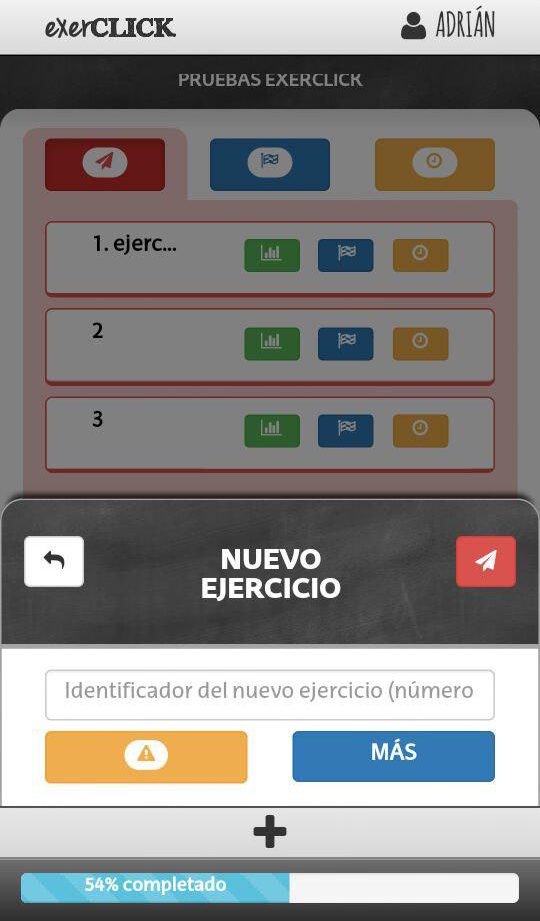
\includegraphics[height=5cm, frame]{ejercicio-simple}
	\caption{Interfaz del UO1-T: Crear-Lanzar un ejercicio simple}
	\label{fig:crear-lanzar-ejercicio-simple}
\end{subfigure}
%
\begin{subfigure}[t]{0.7\textwidth}
	\centering
	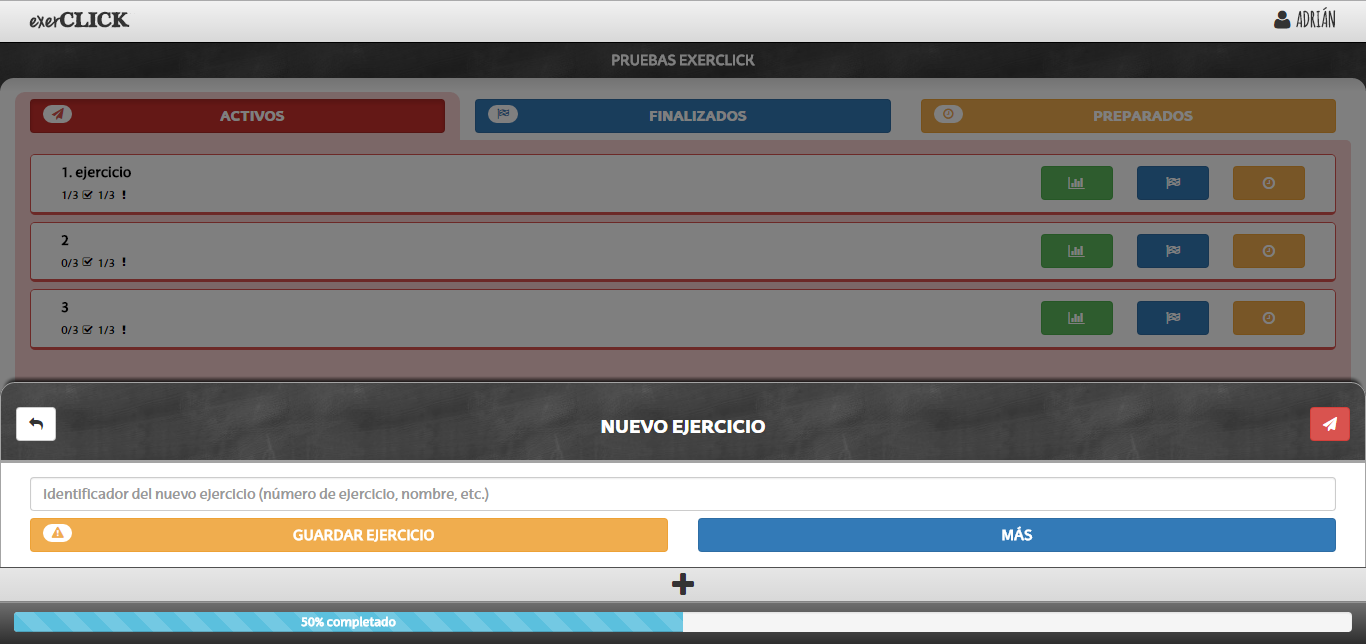
\includegraphics[height=5cm, frame]{P2_big}
	\caption{Versión grande (tablet) de la pantalla del UO1-T (P2\textsubscript{T})}
	\label{fig:crear-lanzar-ejercicio-simple-big}
\end{subfigure}

\caption{Pantallas del UO1-T (P2\textsubscript{T})}
\label{diseno-e-implementacion:interfaces:profesor}
\end{figure}

\subsubsection{UO2-T: Crear-Lanzar un ejercicio detallado}
\label{diseno-e-implementacion:interfaces:profesor:uo2-t}

En la pantalla de la figura \ref{fig:crear-lanzar-ejercicio-avanzados}, correspondiente al P2\textsubscript{T}\textsuperscript{I}, se añaden más detalles a parte del identificador (opcionales todos menos este último). Al pulsar sobre el botón ''Menos'' volveremos a P2\textsubscript{T}.\\

\noindent
\begin{figure}[!htbp]
	\centering
	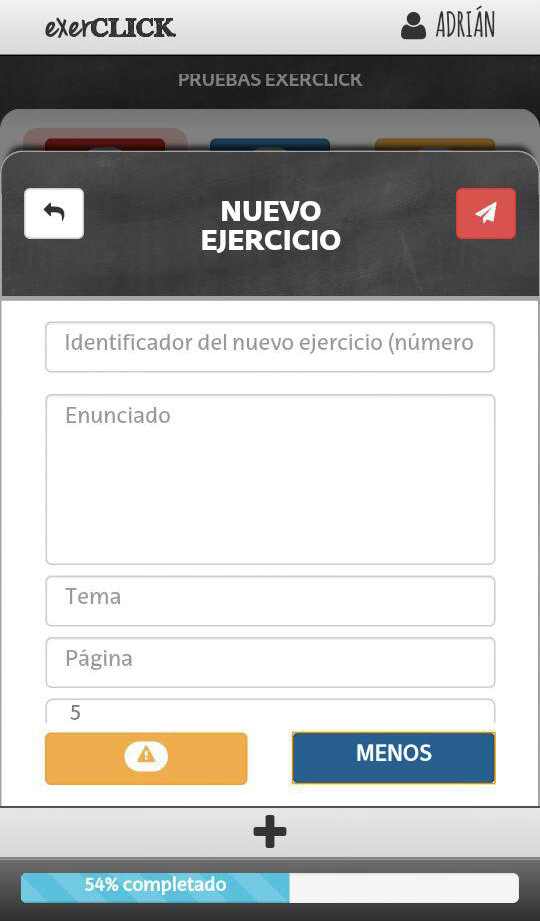
\includegraphics[height=7cm, frame]{ejercicio-avanzado}
	\caption{Interfaz del UO2-T: Crear-Lanzar un ejercicio detallado}
	\label{fig:crear-lanzar-ejercicio-avanzados}
\end{figure}

\subsubsection{UO4-T: Ver estadísticas de un ejercicio}
\label{diseno-e-implementacion:interfaces:profesor:uo4-t}

En la figura \ref{fig:diseno-e-implementacion:interfaces:profesor:uo4-t} vemos todas las pantallas asociadas a las estadísticas de los ejercicios. La parte superior de la nueva pestaña de esta pantalla es similar a la de crear nuevos ejercicios. En la parte central hay 3 botones verdes, un buscador y una lista de alumnos. Al cargar esta pestaña se cargarán todos los alumnos involucrados en el ejercicio (esto corresponde al primer botón). Los otros dos botones muestran todos los alumnos que han marcado el ejercicio como acabado y todos aquellos que han marcado una duda (en ese orden). El buscador nos permite buscar por nombre y/o apellido a cualquier persona (busca por subcadenas, así que no es necesario introducir el nombre o apellido completo) e irá actualizando la lista de alumnos.\\

\noindent
\begin{figure}[!htbp]
\begin{subfigure}[t]{0.3\textwidth}
	\centering
	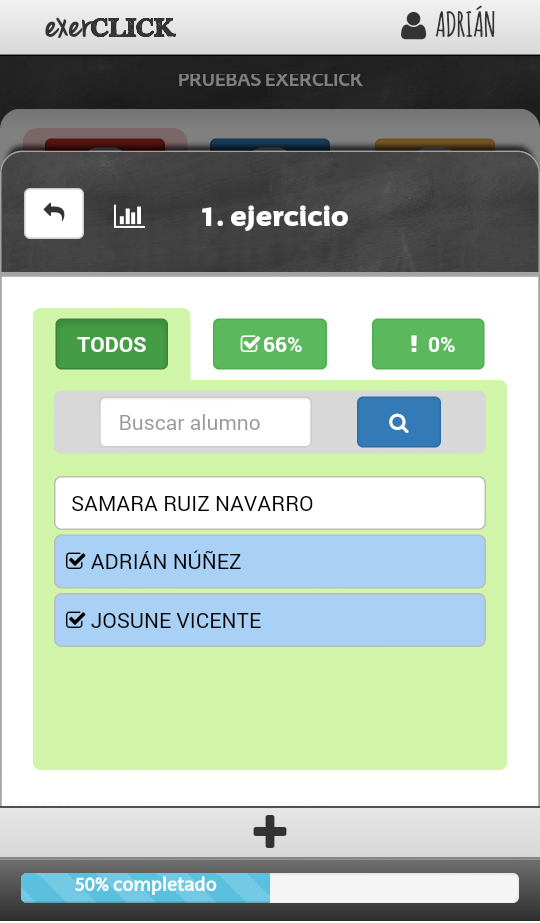
\includegraphics[height=7cm, frame]{P5T}
	\caption{P5T: todos}
	\label{fig:diseno-e-implementacion:interfaces:profesor:uo4-t:p5t}
\end{subfigure}
%
\begin{subfigure}[t]{0.3\textwidth}
	\centering
	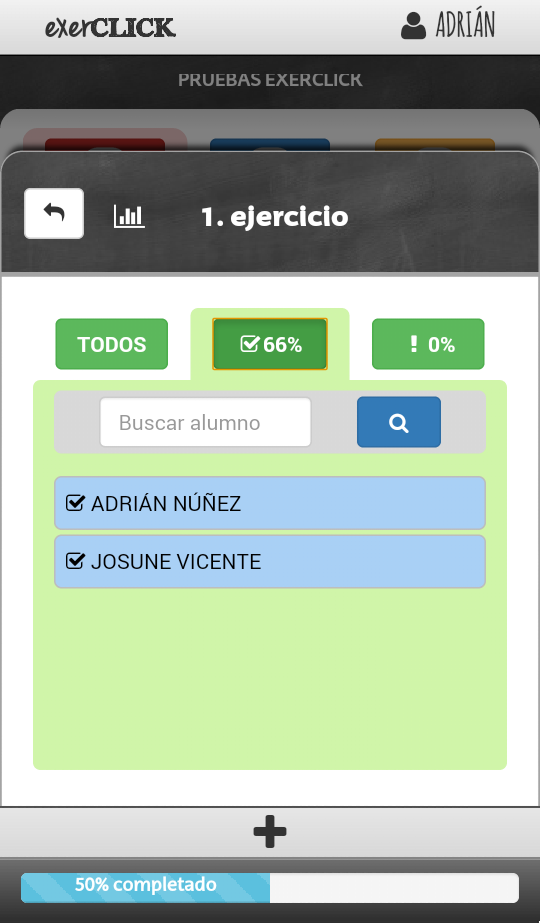
\includegraphics[height=7cm, frame]{P5A}
	\caption{\textsubscript{T}\textsuperscript{A}: sólo acabados}
	\label{fig:diseno-e-implementacion:interfaces:profesor:uo4-t:p5a}
\end{subfigure}
%
\begin{subfigure}[t]{0.3\textwidth}
	\centering
	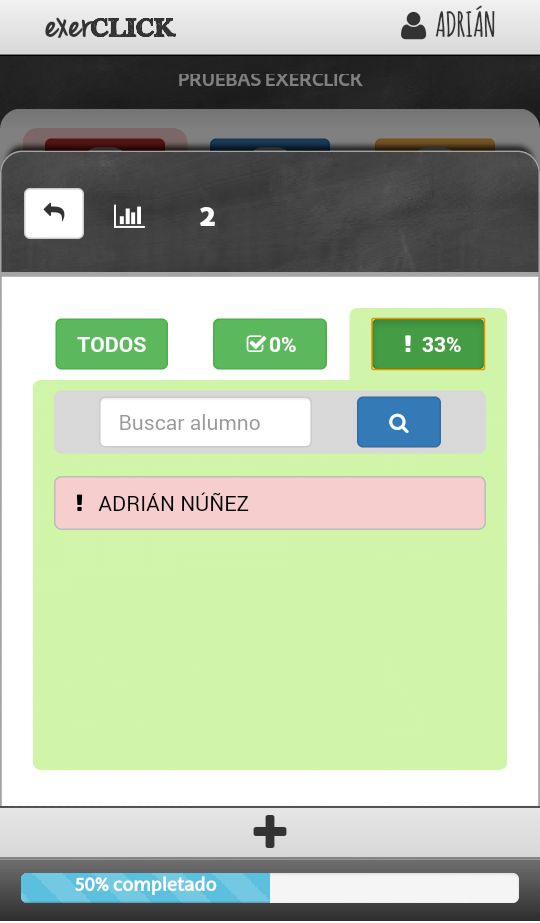
\includegraphics[height=7cm, frame]{P5D}
	\caption{\textsubscript{T}\textsuperscript{D}: sólo con dudas}
	\label{fig:diseno-e-implementacion:interfaces:profesor:uo4-t:p5d}
\end{subfigure}
\\
\begin{subfigure}[t]{\textwidth}
	\centering
	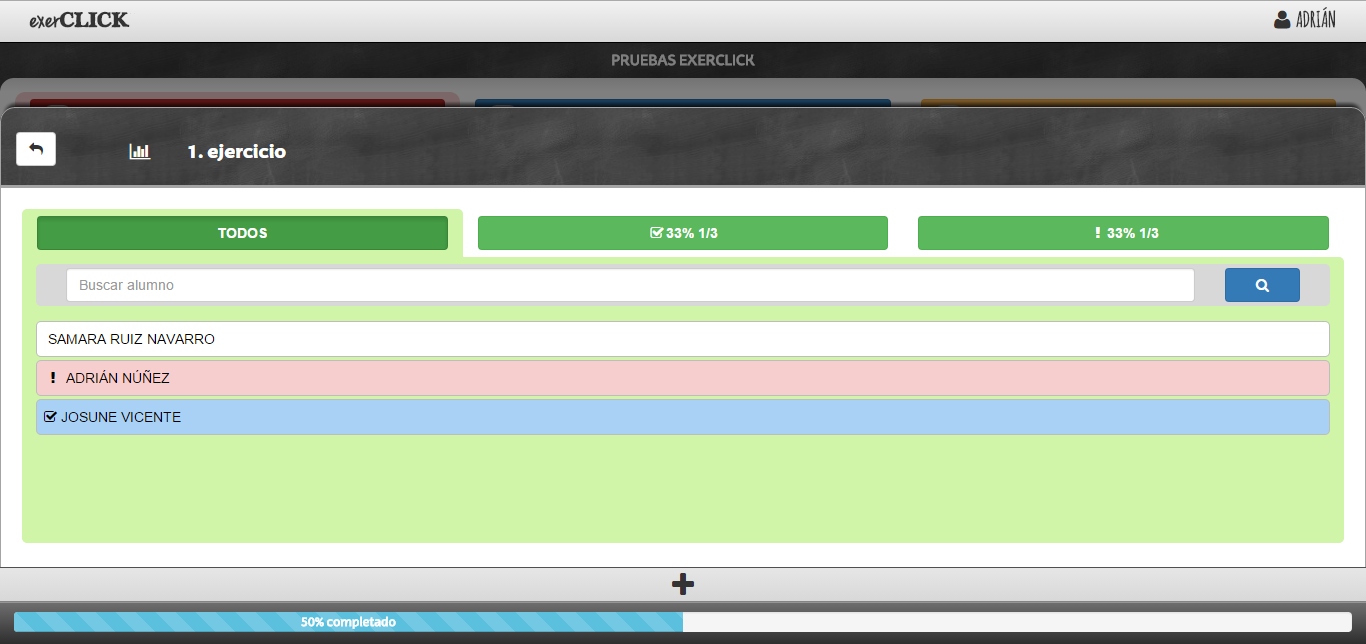
\includegraphics[width=\textwidth, frame]{P5_big}
	\caption{Versión grande (tablet) de la pantalla del UO4-T (P5\textsubscript{T}\textsuperscript{T})}
	\label{fig:diseno-e-implementacion:interfaces:profesor:uo4-t:p5a-big}
\end{subfigure}

\caption{Pantallas del UO4-T (P5\textsubscript{T})}
\label{fig:diseno-e-implementacion:interfaces:profesor:uo4-t}
\end{figure}

\subsubsection{UO5-T: Ver la descripción completa de un ejercicio}
\label{diseno-e-implementacion:interfaces:profesor:uo5-t}

La pantalla para ver los detalles de un ejercicio (P3\textsubscript{T}) se muestra en la figura \ref{fig:diseno-e-implementacion:interfaces:profesor:uo5-t}. En la parte superior vemos un botón azul con engranajes que nos lleva a la pantalla P4\textsubscript{T} (UO6-T). En la parte central veremos los detalles del ejercicio que estamos viendo (si hubiera alguno). Si un ejercicio no tiene detalles aparecerá un mensaje indicando que no existen detalles asociados al ejercicio como en la figura \ref{fig:diseno-e-implementacion:interfaces:profesor:uo5-t:p3'}.\\

\noindent
\begin{figure}[!htbp]
\begin{subfigure}[t]{0.5\textwidth}
	\centering
	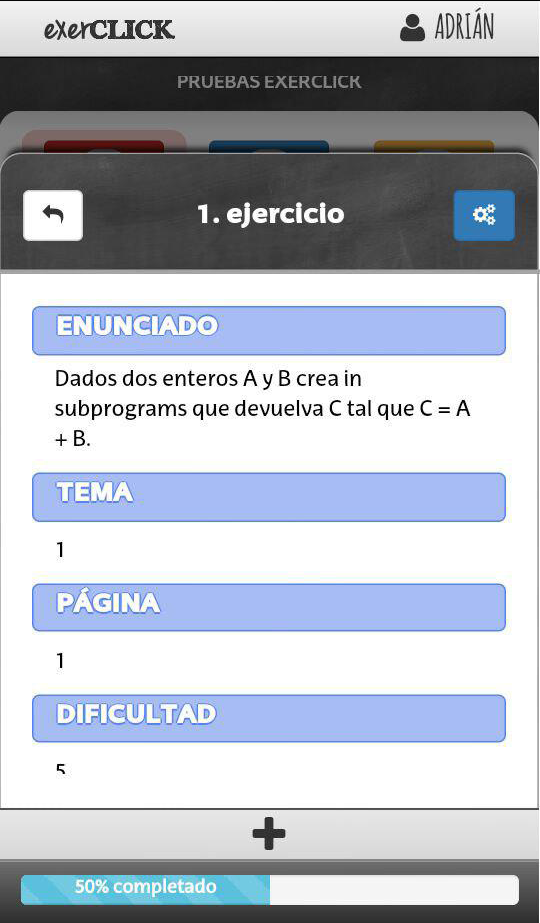
\includegraphics[height=7cm, frame]{P3}
	\caption{P3\textsubscript{T}: ver detalles de un ejercicio}
	\label{fig:diseno-e-implementacion:interfaces:profesor:uo5-t:p3}
\end{subfigure}
%
\begin{subfigure}[t]{0.5\textwidth}
	\centering
	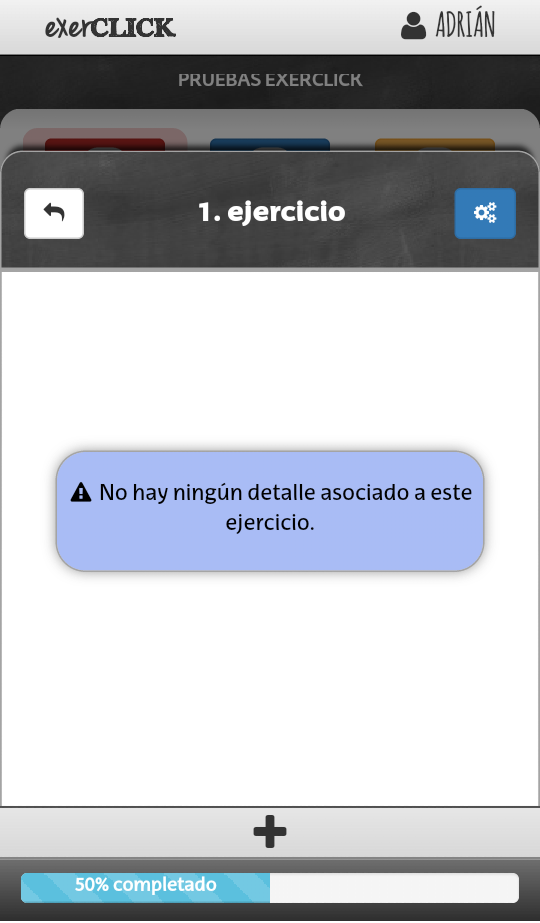
\includegraphics[height=7cm, frame]{P3'}
	\caption{P3\textsubscript{T}: no hay detalles asociados}
	\label{fig:diseno-e-implementacion:interfaces:profesor:uo5-t:p3'}
\end{subfigure}
\\
\begin{subfigure}[t]{\textwidth}
	\centering
	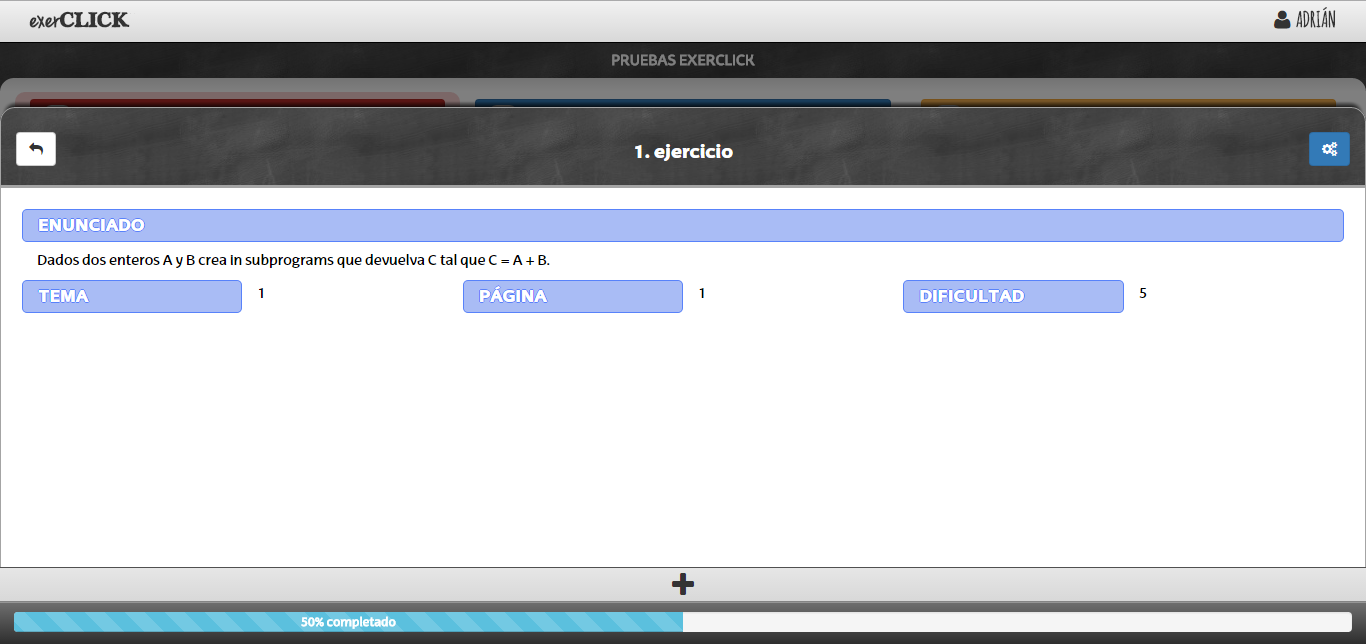
\includegraphics[height=5cm, frame]{P3_big}
	\caption{P3\textsubscript{T}: versión tableta}
	\label{fig:diseno-e-implementacion:interfaces:profesor:uo5-t:p3-big}
\end{subfigure}

\caption{Pantallas del UO5-T (P3\textsubscript{T})}
\label{fig:diseno-e-implementacion:interfaces:profesor:uo5-t}
\end{figure}

\subsubsection{UO6-T: Editar un ejercicio}
\label{diseno-e-implementacion:interfaces:profesor:uo6-t}

Para editar un ejercicio accederemos a la pantalla P4\textsubscript{T} (figura \ref{fig:diseno-e-implementacion:interfaces:profesor:uo6-t}). Para llegar a esta pantalla hay que pulsar sobre el botón de los engranajes en la pantalla P3\textsubscript{T}. Los detalles que antes (en P3\textsubscript{T}) eran texto plano ahora están dentro de un campo editable (incluido el identificador del ejercicio). Si volvemos a pulsar el botón de engranajes no se guardarán los cambios y volveremos a P3\textsubscript{T}. Si pulsamos en el botón ''Guardar cambios'' que hay en la parte de abajo se guardarán y volveremos a P3\textsubscript{T} con los datos modificados.\\

\noindent
\begin{figure}[!htbp]
\begin{subfigure}[t]{0.5\textwidth}
	\centering
	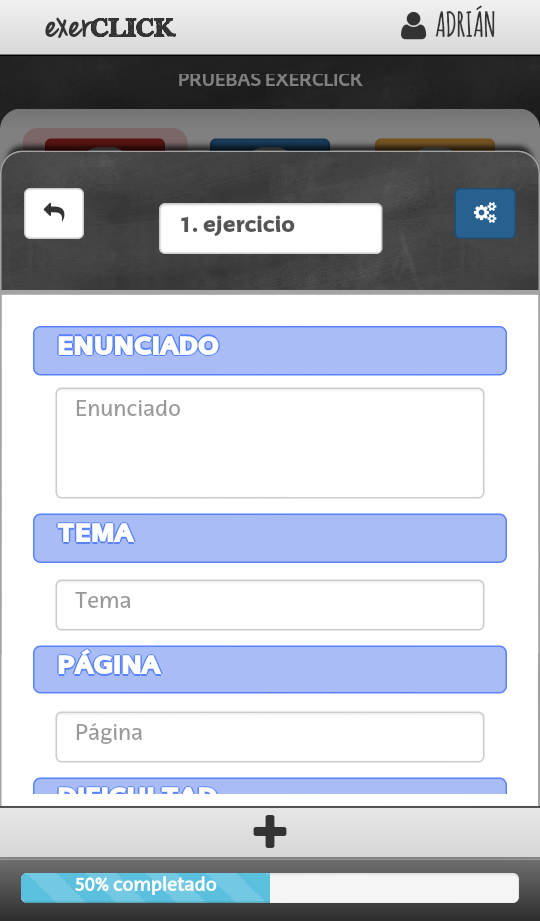
\includegraphics[height=7cm, frame]{P4-2}
	\caption{P4: editar un ejercicio}
	\label{fig:diseno-e-implementacion:interfaces:profesor:uo6-t:p4}
\end{subfigure}
%
\begin{subfigure}[t]{0.5\textwidth}
	\centering
	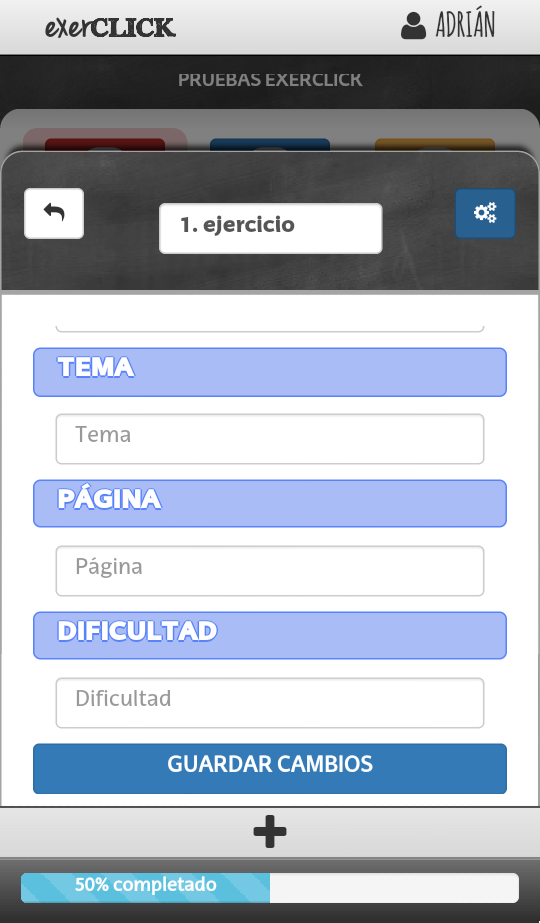
\includegraphics[height=7cm, frame]{P4}
	\caption{P4: editar un ejercicio (\textit{scroll down})}
	\label{fig:diseno-e-implementacion:interfaces:profesor:uo6-t:p4'}
\end{subfigure}

\caption{Pantallas del UO6-T (P4\textsubscript{T})}
\label{fig:diseno-e-implementacion:interfaces:profesor:uo6-t}
\end{figure}

\subsection{Uso de iconos mediante Font Awesome}
\label{diseno-e-implementacion:interfaces:font-awesome}

Font Awesome \hyperref[fontawesome]{\cite{fontawesome}} es un sitio web generado mediante un repositorio de Github. De este sitio se han obtenido todos los iconos de la aplicación: desde los iconos de los botones hasta el icono de usuario que aparece junto al nombre de usuario.\\

Su uso es sencillo, para añadir cualquier icono basta con añadir código como el de este ejemplo (para añadir el icono del avión de papel de los ejercicios activos):\\

\begin{lstlisting}[frame=single]
<i class="fa fa-paper-plane"></i>
\end{lstlisting}

Además podemos aumentar el tamaño del icono añadiendo clases del tipo fa-2x, fa-3x, etc. (aumentan por 2 y por 3 el tamaño del icono, respectivamente). También existe la opción de adaptarlo al texto que tiene cerca con fa-fw y otras tantas opciones que no se han llegado a utilizar en el proyecto (rotaciones, añadir un marco de prohibido encima, etc.). Se pueden encontrar ejemplos en la propia página.\\

\section{M-3: Lógica de negocio o lado del servidor}
\label{diseno-e-implementacion:logica-negocio}

En esta sección hablaremos sobre el código del lado del servidor (escrito en PHP) desde el apartado \ref{diseno-e-implementacion:configuracion} hasta el \ref{diseno-e-implementacion:logica-negocio:cambiar-asignatura} y sobre la base de datos en el apartado \ref{diseno-e-implementacion:logica-negocio:bd}.\\

\subsection{Configuración}
\label{diseno-e-implementacion:configuracion}

\noindent
\begin{lstlisting}[caption=Autenticación del usuario.,label={lst:autenticacion}]
<?php
	define('HOST', 'xxxx');
	// Database username
	define('USER', 'xxxx');
	// Database password
	define('PASSWORD', 'xxxx');
	// Database name
	define('DATABASE', 'xxxx'); 
	 
	define("CAN_REGISTER", "any");
	define("DEFAULT_ROLE", "member");
?>
\end{lstlisting}

Este archivo de configuración define datos de autenticación en la base de datos. Se añade y utiliza en cada fichero mediante el siguiente código:

\noindent
\begin{lstlisting}[caption=Autenticación del usuario.,label={lst:autenticacion}]
include 'mysqli-config.php';
$mysqli = new mysqli(HOST, USER, PASSWORD, DATABASE);

if (mysqli_connect_errno()) {
     echo "Failed to connect to MySQL: " . mysqli_connect_error();
}
\end{lstlisting}

Este trozo de código se añade siempre al inicio de cada código PHP en el servidor. Al final se cierra la base de datos.\\

\subsection{Identificación de usuario}
\label{diseno-e-implementacion:logica-negocio:identificacion}

El código \ref{lst:autenticacion} se ejecuta en la interfaz P0 al intentar autenticarse. No se puede tener más de una sesión abierta en diferentes dispositivos, sólo la última sesión es la que se puede utilizar. En la base de datos proporcionada teníamos la tabla \textit{usersession} para almacenar las sesiones y mantener ese control. En esta tabla guardamos el ID de usuario global (almacenado en la tabla \textit{fosUser}) y el identificador de sesión generado por PHP. Además, dependiendo del rol del usuario se le llevará a la interfaz teacher.html o student.html.\\

\noindent
\begin{lstlisting}[caption=Autenticación del usuario.,label={lst:autenticacion}]
$name = test_input($_GET['Username']);
$pass = test_input($_GET['Password']);
   
// Check if username exists
$statement = 'SELECT * FROM fos_user WHERE username="' . $name . '"'; 
$result = $mysqli->query($statement);

// Only 1 result, otherwise error
$num = mysqli_num_rows($result);
if($num != 1){
     die();
}

$row = mysqli_fetch_assoc($result);
if(!isPasswordValid($row['password'], $pass, $row['salt'])) {
     die();
}
// Mandatory call for using $_SESSION array
session_start();
$_SESSION['name'] = $row['username'];

// Check for the role of the user
if (strpos($row['roles'], 'ROLE_STUDENT') !== false) {
     $_SESSION['role'] = "ROLE_STUDENT";
}
if (strpos($row['roles'], 'ROLE_TEACHER') !== false) {
     $_SESSION['role'] = "ROLE_TEACHER";
}

// Save the user id
$_SESSION['general_id'] = $row['id'];
  
// Find id based in role
switch($_SESSION['role']) {
case 'ROLE_STUDENT':
     $statement = 'SELECT id, name, surname1, surname2 FROM student WHERE fosUser="' . $row['id'] . '"';
     $next_location = 'student.html';
     break;	
case 'ROLE_TEACHER':
     $statement = 'SELECT id, name, surname1, surname2 FROM teacher WHERE fosUser="' . $row['id'] . '"';
     $next_location = 'teacher.html';
     break;
}    

$result = $mysqli->query($statement);
if(!$result) {
     die('The query has encounter a problem: ' . mysqli_error($mysqli));
}
  
// Only 1 result, otherwise error
$num = mysqli_num_rows($result);
if($num != 1){
     session_destroy();
     die('No role asigned.');
}
\end{lstlisting}

\subsection{Cargar la interfaz principal (P1 del profesor y P1 del alumno)}
\label{diseno-e-implementacion:logica-negocio:carga}

Es importante al cargar la interfaz saber si tenemos clase o no. Se utiliza principalmente el código \ref{lst:get-data} para ello. Si no hay ninguna guardada en la sesión abierta buscamos si en el día y hora en la que nos encontramos hay alguna clase. Si la hay guardamos el identificador de su \textit{attendanceclass}. En caso de que haya una clase activa simplemente obtendremos datos de ella (hora de inicio, de final y día).\\

Si nos hemos autenticado con el rol de profesor también obtendremos todas sus asignaturas, de modo que podamos cargarlas en el perfil del profesor más adelante.\\

\noindent
\begin{lstlisting}[caption=Obtener información inicial para la carga de la interfaz.,label={lst:get-data}]
if(!isset($_SESSION['class'])) {
     $now = date('H:i');
     $day = date('Y-m-d');
     // Find all classes previous to the actual time
     $statement = 'SELECT * FROM attendanceclass WHERE day <= "' . $day . '" OR (day = "' . $day . '" AND endHour < "' . $now . '") ORDER BY day DESC, startHour DESC';
		
     if(!($result = $mysqli->query($statement))) {
         die('The query has encounter a problem: ' . mysqli_error($mysqli));
     }
		
     $class = -1;
     while($row =  mysqli_fetch_array($result)) {
         // For the next class previous to the actual time find a session given by the logged teacher
         $statement = 'SELECT session.* FROM session INNER JOIN groupteacher ON session.ctGroup = groupteacher.ctGroup WHERE session.id = "' . $row['session'] . '" AND groupteacher.teacher= "' . $_SESSION['id'] . '"';
         if(!($session = $mysqli->query($statement))){
		      die('The query has encounter a problem: ' . mysqli_error($mysqli));
         }
         $group = mysqli_fetch_array($session);
         if(mysqli_num_rows($session) != 0){
              break;
         }
     }
     // Id of the session (next class)
     $class = $row['id'];
} else {
     $class = $_SESSION['class'];
     $statement = 'SELECT * FROM attendanceclass WHERE id= "' . $_SESSION['class'] . '"';
	  
     if(!($result = $mysqli->query($statement))){
          die('The query has encounter a problem: ' . mysqli_error($mysqli));
     }

     $row =  mysqli_fetch_array($result);
     $start = date('H:i', strtotime($row['startHour']));
     $end = date('H:i', strtotime($row['endHour']));
     $day = $row['day'];
}

if($_SESSION['role'] == 'ROLE_TEACHER') {
     $statement = 'SELECT subject.id, subject.name AS subject, subject.acronym, ctgroup.name, ctgroup.id AS group_id FROM subject INNER JOIN ctgroup ON ctgroup.subject = subject.id INNER JOIN groupteacher ON groupteacher.ctgroup = ctgroup.id WHERE groupteacher.teacher= "' . $_SESSION['id'] . '" ORDER BY subject.name ASC';
     if(!($subjects = $mysqli->query($statement))) {
	      die('The query has encounter a problem: ' . mysqli_error($mysqli));
     }
     $subj = array();
     while($row = mysqli_fetch_array($subjects)) {
          $subj[] = array('name' => $row['subject'], 'acronym' => $row['acronym'], 'group' => $row['name'], 'group_id' => $row['group_id'], 'id' => $row['id']);
     }
}
\end{lstlisting}

El segundo elemento principal al cargar las interfaces es la carga de los ejercicios (como se puede ver en el código \ref{lst:carga-ejercicios}. Se obtienen los ejercicios en los que estamos involucrados (porque estamos matriculados en esa asignatura como alumno o porque la impartimos como profesor). Después, independientemente del rol del usuario autenticado, obtenemos para cada ejercicio que hemos obtenido de la base de datos: el número de alumnos que lo han marcado como acabado, el número de ellos que han marcado una duda y el número de alumnos total involucrados en el ejercicio.\\

\noindent
\begin{lstlisting}[caption=Cargar los ejercicios del tipo pasado por parámetro.,label={lst:carga-ejercicios}]
if($_SESSION['role'] == 'ROLE_TEACHER') {
     $statement = 'SELECT exercise.id, description FROM exercise LEFT JOIN ctgroup ON exercise.ctGroup = ctgroup.id INNER JOIN groupteacher ON groupteacher.ctgroup = ctgroup.id ' .
                           'WHERE type = "' . $_GET['Type'] . '" AND ctgroup.id = "' . $_SESSION['group_id'] . '" AND ctgroup.subject = "' . $_SESSION['subject_id'] . '" AND groupteacher.teacher = "' . $_SESSION['id'] . '"';
} else if($_SESSION['role'] == 'ROLE_STUDENT') {
     $statement  = 'SELECT exercise.id, description, state FROM exercise INNER JOIN ctgroup ON ctgroup.id = exercise.ctGroup INNER JOIN groupstudent ON groupstudent.ctgroup = exercise.ctgroup ' .
                           'INNER JOIN exercisestate ON exercise.id = exercisestate.idexercise WHERE type = "Active" AND exercisestate.idstudent = "' . $_SESSION['id'] . '" AND ctgroup.subject = "' . $_SESSION['subject_id'] . '" AND exercise.ctGroup = "' . $_SESSION['group_id'] . '" AND groupstudent.student = "' . $_SESSION['id'] . '"';
}

$result = $mysqli->query($statement);

$exercises = array();
while ($row = $result->fetch_assoc()) {
     $statement = 'SELECT * FROM exercise INNER JOIN exercisestate ON exercise.id = exercisestate.idexercise INNER JOIN ctgroup ON ctgroup.id = exercise.ctGroup ' .
                           'WHERE exercise.id = "' . $row['id'] . '" AND state = "Finished" AND ctgroup.id = "' . $_SESSION['group_id'] . '" AND ctgroup.subject = "' . $_SESSION['subject_id'] . '"';
     $result2 = $mysqli->query($statement);

     $statement = 'SELECT * FROM exercise INNER JOIN exercisestate ON exercise.id = exercisestate.idexercise INNER JOIN ctgroup ON ctgroup.id = exercise.ctGroup ' .
                           'WHERE exercise.id = "' . $row['id'] . '" AND state = "Question" AND ctgroup.id = "' . $_SESSION['group_id'] . '" AND ctgroup.subject = "' . $_SESSION['subject_id'] . '"';
     $result3 = $mysqli->query($statement);

     $statement = 'SELECT * FROM exercise INNER JOIN attendanceclass ON exercise.launched = attendanceclass.id INNER JOIN attendanceclassstudent ON attendanceclassstudent.attendanceclass = attendanceclass.id WHERE exercise.id = "' . $row['id'] . '"';
     $result4 = $mysqli->query($statement);
               
     $row['nofinished'] = mysqli_num_rows($result2);
     $row['noquestions'] = mysqli_num_rows($result3);
     $row['num'] = mysqli_num_rows($result4);
                
     $exercises[] = array('exercise' => $row);
}
\end{lstlisting}

Ambas interfaces principales también comparten las barras de progreso de la clase. Para obtener la información para cargarlas se ejecuta el código \ref{lst:progress-bar-info-teacher} en el caso del profesor y el \ref{lst:progress-bar-info-student} en el caso del alumno. Nos devuelven el porcentaje de carga para cada barra mediante simples divisiones.\\

\noindent
\begin{lstlisting}[caption=Obtener información para la carga de la barra de progreso del profesor.,label={lst:progress-bar-info-teacher}]
$statement = 'SELECT * FROM exercise INNER JOIN ctgroup ON ctgroup.id = exercise.ctGroup ' .
                           'WHERE ctgroup.id = "' . $_SESSION['group_id'] . '" AND ctgroup.subject = "' . $_SESSION['subject_id'] . '" AND exercise.type != "Ready"';
$result = $mysqli->query($statement);
$total = mysqli_num_rows($result);

$statement = 'SELECT * FROM exercise INNER JOIN ctgroup ON ctgroup.id = exercise.ctGroup ' .
                           'WHERE ctgroup.id = "' . $_SESSION['group_id'] . '" AND ctgroup.subject = "' . $_SESSION['subject_id'] . '" AND exercise.type = "Finished"';
$result = $mysqli->query($statement);
$finished = mysqli_num_rows($result);
\end{lstlisting}

\noindent
\begin{lstlisting}[caption=Obtener información para la carga de la barra de progreso del estudiante.,label={lst:progress-bar-info-student}]
$statement  = 'SELECT * FROM exercise INNER JOIN ctgroup ON ctgroup.id = exercise.ctGroup INNER JOIN exercisestate ON exercisestate.idexercise = exercise.id ' .
                           'WHERE ctgroup.id = "' . $_SESSION['group_id'] . '" AND ctgroup.subject = "' . $_SESSION['subject_id'] . '" AND exercisestate.idstudent = "' . $_SESSION['id'] . '"';	
$result = $mysqli->query($statement);
$total = mysqli_num_rows($result);

$statement       = 'SELECT * FROM exercise INNER JOIN ctgroup ON ctgroup.id = exercise.ctGroup INNER JOIN exercisestate ON exercisestate.idexercise = exercise.id ' .
                           'WHERE ctgroup.id = "' . $_SESSION['group_id'] . '" AND ctgroup.subject = "' . $_SESSION['subject_id'] . '" AND exercisestate.idstudent = "' . $_SESSION['id'] . '" AND exercisestate.state = "Finished"';
$result = $mysqli->query($statement);
$finished = mysqli_num_rows($result);

$studentprogress = ($total == 0) ? 0 : intval($finished * 100 / $total);

$statement = 'SELECT * FROM attendanceclassstudent INNER JOIN attendanceclass ON attendanceclass.id = attendanceclassstudent.attendanceclass INNER JOIN session ON attendanceclass.session = session.id INNER JOIN ctgroup ON ctgroup.id = session.ctGroup INNER JOIN exercise ON exercise.ctGroup = ctgroup.id INNER JOIN exercisestate ON exercisestate.idexercise = exercise.id ' .
                     'WHERE ctgroup.id = "' . $_SESSION['group_id'] . '" AND ctgroup.subject = "' . $_SESSION['subject_id'] . '"';
$result = $mysqli->query($statement);
$total = mysqli_num_rows($result);

$statement = 'SELECT * FROM attendanceclassstudent INNER JOIN attendanceclass ON attendanceclass.id = attendanceclassstudent.attendanceclass INNER JOIN session ON attendanceclass.session = session.id INNER JOIN ctgroup ON ctgroup.id = session.ctGroup INNER JOIN exercise ON exercise.ctGroup = ctgroup.id INNER JOIN exercisestate ON exercisestate.idexercise = exercise.id ' .
                      'WHERE ctgroup.id = "' . $_SESSION['group_id'] . '" AND ctgroup.subject = "' . $_SESSION['subject_id'] . '" AND exercisestate.state = "Finished"';
$result = $mysqli->query($statement);
$finished = mysqli_num_rows($result);
\end{lstlisting}

\subsection{Responder a un ejercicio (UO1-S)}
\label{diseno-e-implementacion:logica-negocio:responder-ejercicio}

Un alumno puede marcar un ejercicio como acabado o con una duda. Este nuevo estado s pasa por parámetro y se procesa con el código \ref{lst:responder-ejercicio}.\\

Si el ejercicio estaba con una duda marcada y la quitamos inmediatamente debemos guardarlo en la base de datos como una duda resuelta (estas dudas resueltas se muestran en las estadísticas de los ejercicios finalizados). Si el ejercicio ya tenía una duda resuelta anteriormente por el estudiante se actualiza y se guarda la última.\\

\noindent
\begin{lstlisting}[caption=Responder a un ejercicio.,label={lst:responder-ejercicio}]
$idexercise = $_GET['Idexercise'];
$idstudent = $_SESSION['id'];
$state = $_GET['State'];

$statement = 'SELECT state FROM exercisestate WHERE idexercise = "' . $idexercise . '" AND idstudent = "' . $idstudent . '"';
$result = $mysqli->query($statement);
$row = $result->fetch_assoc();
if($row['state'] == 'Question' && ($state == 'Nothing' || $state == 'Finished')) {
     $statement = 'SELECT * FROM exercise_solved_questions WHERE idexercise = "' . $idexercise . '" AND idstudent = "' . $idstudent . '"';
     $result = $mysqli->query($statement);
	
     $day = date('Y-m-d');
     $time = date('H:i:s');
     if(mysqli_num_rows($result) == 1) {
          $statement = 'UPDATE exercise_solved_questions SET day = "' . $day . '" AND time = "' . $time . '" WHERE idexercise = "' . $idexercise . '" AND idstudent = "' . $idstudent . '"';
          $mysqli->query($statement);
     } else {
          $statement = 'INSERT INTO exercise_solved_questions (idexercise, idstudent, day, time) VALUES ("' . $idexercise . '", "' . $idstudent . '", "' . $day . '", "' . $time . '")';
          $mysqli->query($statement);
     }
}
$statement = 'UPDATE exercisestate SET state = "' . $state . '" WHERE idexercise = "' . $idexercise . '" AND idstudent = "' . $idstudent . '"';
$result = $mysqli->query($statement);
\end{lstlisting}

\subsection{Ver detalles de un ejercicio (UO2-S y UO5-T)}
\label{diseno-e-implementacion:logica-negocio:ver-detalles-ejercicio}

Al cargar la interfaz P3 (profesor) o P2 (alumno) para ver los detalles de un ejercicio en concreto se cargan a su vez varios datos. Para obtener estos datos se usa el código \ref{lst:ver-detalles-ejercicio}. Mediante el identificador del ejercicio se obtienen todos los campos de un ejercicio y se devuelven. De esta forma desde javascript se pueden añadir los detalles que no sean nulos o vacíos.\\

\noindent
\begin{lstlisting}[caption=Ver detalles de un ejercicio.,label={lst:ver-detalles-ejercicio}]
$statement = 'SELECT * FROM exercise WHERE id = "' . $_GET['Id'] . '"';
$result = $mysqli->query($statement);
$row = $result->fetch_assoc();
\end{lstlisting}

\subsection{Crear-Lanzar un ejercicio (UO1-T y UO2-T)}
\label{diseno-e-implementacion:logica-negocio:crear-lanzar-ejercicio}

El código \ref{lst:crear-lanzar-ejercicio} implementa la función de lanzar ejercicios, ya sean simples o avanzados (con más detalles). En principio se añade un ejercicio en la base de datos con todos sus campos siempre. Cuando creamos un ejercicio simple solo le pasamos (como detalle) el identificador. Al crear un ejercicio avanzado se le pueden pasar más detalles.\\

\noindent
\begin{lstlisting}[caption=Crear-lanzar un ejercicio.,label={lst:crear-lanzar-ejercicio}]
$statement = 'INSERT exercise(ctGroup, type, launched, description, statement, topic, page, difficulty) VALUES ("' . $_SESSION['group_id'] . '", "' . $_GET['State'] . '", "' . $_SESSION['attendanceclass'] . '", "' . $_GET['Description'] . '", "' . $_GET['Statement'] . '", "' . $_GET['Topic'] . '", "' . $_GET['Page'] . '", "' . $_GET['Difficulty'] . '")';
$mysqli->query($statement);

$idexercise = $mysqli->insert_id;

$statement = 'SELECT student FROM groupstudent WHERE groupstudent.ctGroup = "' . $_SESSION['group_id'] . '"';
$result = $mysqli->query($statement);

while ($row = $result->fetch_assoc()) {
     $statement = 'INSERT exercisestate (idstudent, idexercise, state) VALUES ("' . $row['student'] . '", "' . $idexercise . '", "Nothing")';
     $mysqli->query($statement);
}
\end{lstlisting}

\subsection{Cambiar detalles de un ejercicio (UO3-T y UO6-T)}
\label{diseno-e-implementacion:logica-negocio:cambiar-ejercicio}

El código \ref{lst:cambiar-ejercicio} actualiza el estado de un ejercicio con los parámetros que se le pasan, entre ellos el tipo. Dependiendo de los parámetros pasados este código servirá para implementar el UO3-T (cambiar el tipo de un ejercicio) o el UO6-T (editar un ejercicio). Si sólo le pasamos el tipo ejecutará el código correspondiente al UO3-T (línea \ref{line:diseno-e-implementacion:logica-negocio:cambiar-ejercicio:uo3-t}). De otro modo ejecutará la parte correspondiente al UO6-T (línea \ref{line:diseno-e-implementacion:logica-negocio:cambiar-ejercicio:uo6-t}).

\noindent
\begin{lstlisting}[caption=Cambiar el tipo de un ejercicio.,label={lst:cambiar-ejercicio}]
if(!isset($_GET['Description'])  || $_GET['Description'] == null) {
|\label{line:diseno-e-implementacion:logica-negocio:cambiar-ejercicio:uo3-t}|
     $statement = 'SELECT type FROM exercise WHERE id = "' . $_GET['Id'] . '"';
     $result = $mysqli->query($statement);
     $row = $result->fetch_assoc();
     if($row['type'] == 'Ready') {
          $statement = 'UPDATE exercise SET type = "' . $_GET['Type'] . '", launched = "' . $_SESSION['attendanceclass'] . '" WHERE id = "' . $_GET['Id'] . '"';
     } else {
          $statement = 'UPDATE exercise SET type = "' . $_GET['Type'] . '" WHERE id = "' . $_GET['Id'] . '"';

     }
} else {
|\label{line:diseno-e-implementacion:logica-negocio:cambiar-ejercicio:uo6-t}|
     $statement = 'UPDATE exercise SET description = "' . $_GET['Description'] . '", statement = "' . $_GET['Statement'] . '", topic = "' . $_GET['Topic'] . '", page = "' . $_GET['Page'] . '", difficulty = "' . $_GET['Difficulty'] . '" WHERE id = "' . $_GET['Id'] . '"';
}
\end{lstlisting}
 
\subsection{Ver estadísticas un ejercicio (UO4-T)}
\label{diseno-e-implementacion:logica-negocio:estadisticas} 

El código \ref{lst:estadisticas} ejecuta una consulta sobre la base de datos para obtener para un ejercicio en concreto el nombre completo de cada alumno que está involucrado y su estado en él (si lo ha acabado o tiene una duda). Además permite filtrar por nombre o apellido gracias al \textit{Key} pasado por parámetro (utilizando el operador LIKE de SQL). El resultado será mostrado en la interfaz P5.\\

\noindent
\begin{lstlisting}[caption=Obtener estadísticas de un ejercicio.,label={lst:estadisticas}]
$statement = 'SELECT name, surnames, state FROM student INNER JOIN exercisestate ON student.id = exercisestate.idstudent WHERE exercisestate.idexercise = "' . $_GET['Id'] . '" AND state LIKE "' . $_GET['State'] . '" AND (name LIKE "' . $_GET['Key'] . '" OR surnames LIKE "' . $_GET['Key'] . '")';
$result = $mysqli->query($statement);

$statistics = array();
while ($row = $result->fetch_assoc()) {
     $statistics[] = array('statistic' => $row);
}
\end{lstlisting}

Al visualizar las estadísticas de un ejercicio, en cada pestaña se ven los porcentajes de alumnos que han marcado el ejercicio como acabado o que han marcado una duda. Para obtener esos porcentajes se llama al código \ref{lst:estadisticas-2}.\\

\noindent
\begin{lstlisting}[caption=Obtener porcentajes para las estadísticas e un ejercicio.,label={lst:estadisticas-2}]
$data = array();

$statement = 'SELECT * FROM exercisestate INNER JOIN student ON exercisestate.idstudent = student.id WHERE exercisestate.idexercise = ' . $_GET['Id'];
$result = $mysqli->query($statement);
$total = mysqli_num_rows($result);
$data['total'] = $total;
$result->free();
	
$statement = 'SELECT * FROM exercisestate INNER JOIN student ON exercisestate.idstudent = student.id WHERE state LIKE "Finished" AND exercisestate.idexercise = ' . $_GET['Id'];
$result = $mysqli->query($statement);
$finished = mysqli_num_rows($result);
$data['finished'] = $finished;
$result->free();
	
$statement = 'SELECT * FROM exercisestate INNER JOIN student ON exercisestate.idstudent = student.id WHERE state LIKE "Question" AND exercisestate.idexercise = ' . $_GET['Id'];
$result = $mysqli->query($statement);
$question = mysqli_num_rows($result);
$data['question'] = $question;
\end{lstlisting}

Cuando un ejercicio se da por finalizado, al mostrar sus estadísticas veremos una diferencia en el apartado de dudas. Se mostrarán 3 pestañas extra de filtro: mostrar todas las dudas en el ejercicio, mostrar las que no han sido resueltas o mostrar las que alguna vez fueron resueltas (pero luego se marcaron como acabado o quedaron sin marcar). Para poder obtener las estadísticas de esos ejercicios se han utilizado 3 consultas SQL diferentes, algo más complejas. El código \ref{lst:estadisticas-3} devuelve una de las 3 dependiendo del valor del parámetro \textit{Question\_State} que le pasemos.\\

\noindent
\begin{lstlisting}[caption={Mostrar todas las dudas, las no resueltas o las resueltas.},label={lst:estadisticas-3}]
if($_GET['Question_State'] == 'All') {
     $statement = 'SELECT DISTINCT * FROM student INNER JOIN exercisestate ON student.id = exercisestate.idstudent WHERE exercisestate.idexercise = "' . $_GET['Id'] . '" AND exercisestate.state = "Question" AND (name LIKE "' . $_GET['Key'] . '" OR surnames LIKE "' . $_GET['Key'] . '")';
} else if($_GET['Question_State'] == 'Solved') {
     $statement = 'SELECT DISTINCT * FROM student INNER JOIN exercisestate ON student.id = exercisestate.idstudent INNER JOIN exercise_solved_questions ON exercisestate.idexercise = exercise_solved_questions.idexercise AND exercise_solved_questions.idstudent = student.id WHERE exercisestate.idexercise = "' . $_GET['Id'] . '" AND exercisestate.state = "Finished" AND (name LIKE "' . $_GET['Key'] . '" OR surnames LIKE "' . $_GET['Key'] . '")';
} else if($_GET['Question_State'] == 'NotSolved') {
     $statement = 'SELECT DISTINCT * FROM student INNER JOIN exercisestate ON student.id = exercisestate.idstudent LEFT JOIN exercise_solved_questions ON exercisestate.idexercise = exercise_solved_questions.idexercise AND exercise_solved_questions.idstudent = student.id WHERE exercisestate.idexercise = "' . $_GET['Id'] . '" AND  exercisestate.state = "Question" AND (name LIKE "' . $_GET['Key'] . '" OR surnames LIKE "' . $_GET['Key'] . '") AND exercise_solved_questions.id IS NULL';
}
$result = $mysqli->query($statement);

$statistics = array();
while ($row = $result->fetch_assoc()) {
     $statistics[] = array('statistic' => $row);
}
\end{lstlisting}

\subsection{Cambiar de idioma (UO9-T)}
\label{diseno-e-implementacion:logica-negocio:cambiar-idioma}

Para cambiar el idioma se llama a este pequeño trozo de código y se devuelve el resultado.\\

\noindent
\begin{lstlisting}[caption=Cambiar el idioma de la aplicación.,label={lst:cambiar-idioma}]
$_SESSION['lang'] = $_GET['Language'];
\end{lstlisting}

\subsection{Cambiar de idioma (UO10-T)}
\label{diseno-e-implementacion:logica-negocio:cambiar-asignatura}

Se cambian los parámetros de la sesión para reflejar que vamos a cambiar la asignatura activa. Esta asignatura es la que se muestra cuando volvemos a clase desde el perfil (de la que se muestran ejercicios). Los parámetros que definen la asignatura (\textit{Subject}, \textit{Id}, \textit{Group\_Id} y \textit{Group}) vienen de la interfaz, donde son almacenados gracias a los atributos ''data-*'' de HTML5.\\

\noindent
\begin{lstlisting}[caption=Cambiar la asignatura activa.,label={lst:cambiar-asignatura}]
$_SESSION['subject'] = $_GET['Subject'];
$_SESSION['subject_id'] = $_GET['Id'];
$_SESSION['group_id'] = $_GET['Group_id'];
$_SESSION['group'] = $_GET['Group'];
\end{lstlisting}

\subsection{Base de datos}
\label{diseno-e-implementacion:logica-negocio:bd}

El diseño de la base de datos se ha realizado considerando la base de datos utilizada en PresenceClick (ver figura \ref{fig:anexo-c:2} del apéndice ~\ref{anexo-c}). En ella hay muchas tablas que no nos han interesado usar en este proyecto, se han utilizado sólo unas pocas.\\

Se han incorporado unas tablas nuevas a la base de datos ya existente para la gestión de ejercicios tal y como se muestra en la figura \ref{fig:anexo-c:1} del apéndice ~\ref{anexo-c}), donde aparecen algo tablas como \textit{student} de PresenceClick relacionadas a tablas nuevas de \textit{\textbf{exerClick}}. Las tablas añadidas son:

\begin{itemize}
\item \textbf{exercise:} contiene los detalles de un ejercicio, el grupo al que pertenece y el estado del ejercicio.
\item \textbf{exercisestate:} guarda el estado de un ejercicio de un alumno concreto.
\item \textbf{exerciseattendanceclass:} relaciona un ejercicio con la sesión de ejercicios (\textit{attendanceclass}) en la que se lanzó el ejercicio.
\item \textbf{exercise\_solved\_questions:} se guarda el momento (día y hora) en el que una duda de un alumno en un ejercicio ha sido resuelta.
\end{itemize}

Se utiliza el prefijo ''exercise'' para denotar que son relativas a \textit{\textbf{exerClick}}.\\

\section{Estructura del proyecto}
\label{diseno-e-implementacion:estructura}

En este apartado se revisara la estructura del proyecto, es decir, los ficheros que componen el proyecto y su estructura de carpetas. En la figura ~\ref{fig:files-1} se muestra la raíz del proyecto:\\

\noindent
\begin{figure}[!htbp]
	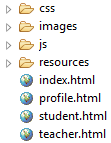
\includegraphics{files-1}
	\caption{Estructura de archivos: raíz del proyecto}
	\label{fig:files-1}
\end{figure}

El proyecto cuenta con 4 carpetas principales: css, js, images y resources. Además contiene 4 ficheros HTML:

\begin{itemize}
\item \textbf{index.html:} funciona como pantalla de identificación de usuario y permite redirigir a las vistas principales (teacher.html o student.html) dependiendo del rol del usuario identificado.
\item \textbf{student.html:} es la vista del alumno.
\item \textbf{teacher.html:} es la vista del profesor.
\item \textbf{profile.html:} pantalla de perfil del profesor, únicamente accesible desde teacher.html.
\end{itemize}

Estos ficheros muestran las interfaces principales de la aplicación. Dentro de las otras carpetas encontramos más ficheros.

\noindent
\begin{figure}[!htbp]
\begin{subfigure}[!htbp]{0.5\textwidth}
	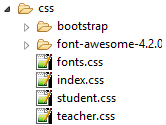
\includegraphics[width=0.6\linewidth]{files-css}
	\caption{Contenido de la carpeta css}
	\label{fig:files-css}
\end{subfigure}
%
\begin{subfigure}[!htbp]{0.5\textwidth}
	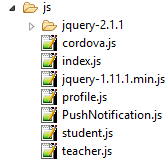
\includegraphics[width=0.6\linewidth]{files-js}
	\caption{Contenido de la carpeta js}
	\label{fig:files-js}
\end{subfigure}
%
\begin{subfigure}[!htbp]{0.5\textwidth}
	
\includegraphics[width=0.6\linewidth]{files-images}
	\caption{Contenido de la carpeta images}
	\label{fig:files-images}
\end{subfigure}
%
\begin{subfigure}[!htbp]{0.5\textwidth}
	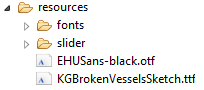
\includegraphics[width=0.6\linewidth]{files-resources}
	\caption{Contenido de la carpeta resources}
	\label{fig:files-resources}
\end{subfigure}

\caption{Contenido de la carpetas principales de la raíz del proyecto}
\label{fig:files-2}
\end{figure}

Los archivos de CSS sirve para darle estilo a las interfaces. Cada interfaz tiene un archivo .css asociado (excepto profile.html, que comparte teacher.css con teacher.html). Además, se añaden dos carpetas extra: la que necesitamos para Boostrap \hyperref[boostrap]{\cite{boostrap}} y para usar los iconos de Font Awesome \hyperref[fontawesome]{\cite{fontawesome}}.\\

Los ficheros Javascript de la carpeta JS le dan dinamicidad a la aplicación. Controlan los clicks, hacen aparecer las pestañas nuevas y cargan contenido dinámicamente mediante AJAX. Cada interfaz (fichero HTML) tiene asociado su propio fichero JS. Además se incluye el fichero cordova.js y los ficheros necesarios para utilizar JQuery.\\

La carpeta images contiene las imágenes utilizadas en el proyecto y la carpeta resources contiene otros elementos utilizados en el proyecto (en este caso fuentes utilizadas).\\

\section{Requisitos de dispositivos para su ejecución}
\label{diseno-e-implementacion:dispositivos}

La aplicación está pensada para el uso en cualquier dispositivo móvil con los sistemas operativos Android e iOS. No está pensada para tamaños de pantalla excesivamente pequeños, donde probablemente la aplicación se vería incorrectamente.\\

En Android la versión mínima requerida es la 4.0 (API 15). En versiones 5.0 o superior no se garantiza que funcione correctamente.\\

%----------------------------------------------------%
%                     CONCLUSIONES                   %
%----------------------------------------------------%

%----------------------------------------------------%
%                     CONCLUSIONES                   %
%----------------------------------------------------%

\pagestyle{fancy}

\chapter{Conclusiones y Líneas futuras}
\label{conclusiones}

\textit{\textbf{exerClick}} es la aplicación para el seguimiento de ejercicios en el aula desarrollada en este proyecto. Su objetivo principal es dar una visión más real de lo que hacen los alumnos (tanto una visión global del grupo como individual), de modo que el docente pueda ofrecer un aprendizaje más adaptado e individualizado, aunque los grupos de alumnos sean muy grandes.\\

Se planteó al inicio como una aplicación web, al igual que su antecesor, qClick \cite{qclick}, una aplicación de pregunta-respuesta en un entorno docente. Se decidió cambiar a una aplicación móvil finalmente, conllevando el cambio en la tecnología principal: \textit{Apache Cordova}. Las tecnologías principales (tecnologías web) se mantuvieron intactas gracias a Cordova: HTML5, CSS3 y Javascript. Ésto permitió realizar una aplicación móvil manteniendo las tecnologías acordadas al inicio del proyecto.\\

El proyecto partió de algo sencillo como idea inicial (objetivo de las primeras iteraciones): una aplicación sencilla de lanzar un ejercicio simple, que el alumno envíe su \textit{feedback} (el estado en el que se encuentra su ejercicio) y el profesor pueda visualizar esa respuesta (tanto de forma individual como grupal, aportando una visión global). Sin embargo, durante la captura de requisitos inicial se vio que había muchas ideas sobre la mesa que podrían ser interesantes, algunas descartadas por requerir quizá demasiado tiempo o ser demasiado ambiciosas. Esto, aun así, aportó gran inspiración para el desarrollo de la aplicación, pudiendo añadir más funcionalidad de forma incremental.\\

El proyecto fue lento al principio debido a la obligación del aprendizaje de la tecnología \textit{Apache Cordova} (y la adaptación de ésta a móviles) y Responsive Web Design. En esta etapa se intentó perfeccionar el objetivo más básico de lanzar un ejercicio, especialmente su interfaz, que había que adaptar muy bien a móviles. Se quería crear también algo reutilizable, de modo que las siguientes interfaces fueran más sencillas de crear. Esto creo un \textit{boom} importante en las fases finales del proyecto, donde se consiguieron crear muchas interfaces y cumplir muchos objetivos en un corto periodo de tiempo.\\

Desde el inicio del proyecto se pensó en tener alumnos evaluando la aplicación, dando un \textit{feedback} más cercano y constante. Debido a lo tarde que apareció una versión útil de la aplicación (que los usuarios pudieran manejar) los alumnos no probaron la aplicación hasta fechas tardías. Incluso hasta poder generar el fichero APK sólo se hicieron pruebas en un único móvil en el que estaba instalada la aplicación (en el anexo \ref{anexo-b} se pueden ver los resultados de esa prueba). Después se les pasó el fichero APK para poder probarla en sus propios móviles, de cara a ver como se adaptaba la aplicación a diferentes dispositivos y de tener un \textit{feedback} más continuo. En este punto no se llevaron acabo evaluaciones presenciales, sólo se recibían opiniones de pruebas por petición del autor o por iniciativa propia de los alumnos. Pese a que no se llevó acabo como fue planeado, las aportaciones recibidas por los usuarios fueron vitales para ciertos errores o para mejorar aspectos importantes de la aplicación.\\

\section{Objetivos alcanzados}

Como se ha comentado, hubo muchas ideas descartadas al inicio por ser demasiado ambiciosas o salirse del alcance previsto del proyecto. Entre los objetivos seleccionados, se han conseguido llevar a cabo satisfactoriamente todos excepto uno, que se comenta en el apartado \ref{step0:uos}.\\

\textbf{Objetivos del Alumno}\\

\textbf{UO1-S:} \textit{Responder a un ejercicio.} El alumno quiere indicar que ha acabado o que tiene dudas con un ejercicio que el profesor ha propuesto. Para ello, se ha pensado en que el alumno puede marcar el ejercicio con uno de los dos estados. A modo de \textit{feedback}, el profesor recibirá el estado (acabado o con dudas) de ese alumno.\\

\textbf{UO2-S:} \textit{Ver detalles de un ejercicio.} El alumno quiere ver más detalles sobre un ejercicio disponible y activo en la sesión. Al pinchar sobre un ejercicio puede ver cualquier detalle extra que el profesor haya decidido añadir.\\

\textbf{Objetivos del Profesor}\\

\textbf{UO1-T:} \textit{Crear-Lanzar un ejercicio simple.} El profesor quiere proponer un ejercicio rápidamente, sin escribir mucho. Ésto resulta especialmente útil cuando se tiene claro cuales son los ejercicios que se mencionan (se sabe el tema, la página... el contexto de qué ejercicios se están realizando es claro) y cuando se quieren lanzar rápidamente sin perder mucho tiempo.\\

\textbf{UO2-T:} \textit{Crear-Lanzar un ejercicio detallado.} El profesor quiere proponer la realización de un ejercicio preparado previamente o con bastantes detalles. Al contrario que en el UO1-T, en este caso el profesor se los puede preparar fuera de una sesión, incluso llegando a inventarse un ejercicio.\\

\textbf{UO3-T:} \textit{Cambiar el tipo de ejercicio.} El profesor desea cambiar un ejercicio del tipo que tiene a otro cualquiera (de activo a finalizado, por ejemplo). Fundamental cuando se desea lanzar un ejercicio que estaba guardado mientras se preparaba mejor, cuando queremos dar un ejercicio por finalizado o cuando nos confundimos en cualquier cambio y queremos deshacerlo.\\

\textbf{UO4-T:} \textit{El profesor desea ver qué tal le ha ido a la clase en general o a un alumno en un ejercicio.} Este UO es quizá de los más importantes, ya que es el que nos muestra todo el \textit{feedback} recibido de los alumnos. Podemos ver el estado de un ejercicio para cada alumno o ver globalmente (en porcentajes) el progreso de la clase.\\

\textbf{UO5-T:} \textit{Ver la descripción completa de un ejercicio.} Un profesor quiere ver la descripción completa de un ejercicio (identificador, enunciado, página, tema, etc.).\\

\textbf{UO6-T:} \textit{Editar un ejercicio.} El profesor desea editar los atributos de un ejercicio. Quizá se haya equivocado al crear el ejercicio en algún detalle o quiera añadir más detalles. Especialmente útil para los ejercicios que se han guardado y se quieren preparar mejor.\\

\textbf{UO8-T:} \textit{Cerrar sesión.} El profesor quiere cerrar su sesión activa.\\

\textbf{UO9-T:} \textit{Cambiar el idioma de la aplicación.} El profesor desea cambiar el idioma con el que lee la aplicación. Un requisito fundamental de cara a la internacionalización fue que la aplicación estuviera en 4 idiomas: castellano, euskera, inglés y francés.\\

\textbf{UO10-T:} \textit{Cambiar de asignatura.} El profesor, que tiene más de una asignatura, quiere cambiar de una asignatura x a otra asignatura y.\\

\section{Líneas futuras y Propuestas de mejora}

\textit{\textbf{exerClick}} fue pensada como parte de un proyecto mayor, \textit{pClick} y a su vez \textit{PresenceClick}, que integrará ésta y otras aplicaciones. Pasaría a tener un módulo en \textit{PresenceClick}, de modo que algunas opciones de \textit{\textbf{exerClick}} que quizá necesiten de un entorno de trabajo más apropiado (como un ordenador) podrían exportarse a ese módulo.\\

Además de ésto, se pensaron más ideas relacionadas a \textit{\textbf{exerClick}} que quedaron en el tintero. La siguiente lista aporta todas esas ideas y otras que surgieron durante o después del desarrollo del proyecto:

\begin{itemize}
\item Evaluar a un alumno en un ejercicio (UO7-T). Este objetivo se marcó como una posibilidad y resultaba interesante. Para un ejercicio se permitía asignarle a un alumno una valoración del 1 al 5 (usando \textit{emoticonos} de tristeza o sonrisa de diferentes grados) al igual que hace \textit{PresenceClick}. El docente se acercaría a un alumno, vería el estado en el que se encuentra con el ejercicio y si al docente le pareciera correcto podría darle una valoración (no visible para el alumno, es algo personal del docente).\\

Otro objetivo diferente sería que el propio alumno pudiera valorarse a si mismo, de modo que cuando un profesor da un ejercicio por finalizado el alumno puede introducir una valoración sobre si mismo.\\

\item Mejorar la autenticación queda abierta para varias mejoras:
\begin{itemize}
\item Mejorar el control de errores como que no haya conexión (con un aviso), por ejemplo.
\item Que a un alumno se le reconozca si se ha identificado en la clase (utilizando el sistema de reconocimiento por tarjeta) y en caso contrario enviar un mensaje de error.
\end{itemize}

\item Poder descargar un PDF con los detalles de los ejercicios, de modo que para ejercicios con muchos detalles se tuviera una visualización más sencilla.

\item Borrar ejercicios por completo. Esta idea se pensó en realizarla desde PresenceClick por seguridad, por eso no se ha implementado.

\item Permitirle al alumno acceder a su propio perfil con las posibilidades de cerrar sesión y cambiar de idioma (al igual que el profesor). Debido a la semejanza entre pantallas no llevaría mucho trabajo añadir esta mejora.

\item Mejorar el uso de Responsive Web Design en pantallas grandes. Se ha usado RWD para adaptar el diseño a cualquier pantalla, enfocándose en una pantalla de un dispositivo móvil. En tablets, por ejemplo, el diseño deja muchos huecos libres sin aprovecharse. Sería interesante aprovechar esos espacios libres para añadir más información. También se podría plantear el diseño de otra manera para aprovechar mejor las pantallas grandes. 
\end{itemize}

Toda la información reunida con exerClick que alimente la base de datos proporcionará datos muy interesantes para futuros usos. Si bien por si sola la información de exerClick no parece demasiado útil, una vez que juntemos esta y la información reunida por los otros módulos tendremos una base de datos con muchísima información para realizar todo tipo de procesos. Podríamos realizar incluso predicciones sobre el rendimiento de los alumnos hacia el final del curso, por ejemplo (lo que viene siendo \textit{Machine Learning}). Se puede usar la información para ver como se podría mejorar una asignatura respecto a entregables, clases, etc. Hay bastantes posibilidades futuras, pero \textit{\textbf{exerClick}} se dejó en este punto como un Trabajo de Fin de Grado, con posibilidades de mejora hacia el futuro.\\

\section{Lecciones aprendidas}

\subsection*{Apache Cordova vs Aplicación Nativa}
\begin{itemize}
\item Basándome en mi experiencia durante el proyecto y en algunas opiniones recogidas me ha parecido que la tecnología de Apache Cordova intenta abarcar demasiado. Las aplicaciones que se generan se vuelven lentas y con fallos. Para un proyecto que quiera un diseño interesante, sin embargo, Cordova es una herramienta sencilla de usar. También para aquellos que no tengan conocimientos de las tecnologías de Android y quieran crear una aplicación esta herramienta es estupenda.\\

Para desarrollar una futura aplicación, en lo personal, tendría en cuenta crear una aplicación nativa de Android. El desarrollo de la interfaz ha sido la parte más costosa de esta aplicación, cosa que con una aplicación nativa es sencillo y robusto, adaptable a cualquier pantalla fácilmente (con Cordova hay que romperse más la cabeza). A parte de eso señalaría también los siguientes motivos:
\begin{itemize}
\item La falta de documentación de Cordova frente a al gran comunidad de Android.
\item Gestores de errores o \textit{plugins} fáciles de instalar y utilizar en Android con Cordova se vuelven una pesadilla.
\end{itemize}
En resumen, escoge Cordova si:
\begin{itemize}
\item No tienes conocimientos de Android.
\item Quieres realizar una aplicación visualmente atractiva con tus conocimientos web.
\item La aplicación es ligera y no va a tener demasiada funcionalidad.
\end{itemize}
Y crea una aplicación nativa en Android si:
\begin{itemize}
\item Va a tener muchas funcionalidades.
\item Vas a manejar muchas animaciones o efectos.
\item Quieres crear algo simple (sin meterte en todo el tema Cordova) o algo realmente amplio (resulta más cómodo para no tener tantos problemas).
\end{itemize}
\end{itemize}

\subsection*{Generar un apk con Apache Cordova}

Para generar un apk necesitaremos usar un IDE de desarrollo, en este caso se usó Eclipse Luna. Crearemos un nuevo proyecto en Android con el código que tenemos (si no estábamos trabajando ya sobre un IDE) tal y como se muestra en la figura \ref{fig:LLAA-1}.\\

\begin{figure}[!htbp]
	\centering
	\includegraphics[width=\textwidth]{LLAA_1}
	\caption{Primer paso: crear un proyecto nuevo}
	\label{fig:LLAA-1}
\end{figure}

En el proyecto nuevo debemos meter nuestro código en la ruta ''\textit{assets/www}'' (si no existe cread las carpeta necesarias). También necesitaremos el archivo cordova.js que podemos conseguir en https://github.com/apache/cordova-js. Deberíamos tener algo parecido a la estructura de la figura \ref{fig:LLAA-2}.\\

\begin{figure}[!htbp]
	\centering
	\includegraphics[height=10cm]{LLAA_2}
	\caption{Segundo paso: tener la estructura y archivos correctos}
	\label{fig:LLAA-2}
\end{figure}

Finalmente debemos ejecutar el proyecto (aunque no llegue a cargarse el emulador, para hacerlo rápido podemos anular el proceso cuando se nos pida escoger el emulador). Una vez ejecutado se habrá creado el apk y podremos encontrar en la carpeta bin de nuestro proyecto de Eclipse (figura \ref{fig:LLAA-2}).\\

%----------------------------------------------------%
%                    BIBLIOGRAFIA                    %
%----------------------------------------------------%

\nocite{*}
\printbibliography[heading=bibintoc,title={Bibliografía y Referencias}]

%----------------------------------------------------%
%                    APENDICES                       %
%----------------------------------------------------%

% Reiniciamos el contador de capítulos
\setcounter{chapter}{0}
\renewcommand{\chaptername}{Apéndice}
\renewcommand{\thechapter}{\Alph{chapter}}

\pagestyle{fancy}

\chapter{Actas de Reunión}
\label{anexo-a}

\section*{Reunión de Trabajo 1}

\textbf{Fecha:} 8 de octubre de 2014\\

\textbf{Hora de inicio:} 12:30\\

\textbf{Hora de finalización:} 13:45\\

\textbf{Presentes:} Maite Urretavizcaya, Adrián Núñez\\

\textbf{Temas tratados durante la reunión:}

\begin{itemize}
\item Inicio del proyecto: presentación del proyecto y de la metodología de trabajo a seguir durante el desarrollo del 	mismo.
\item Acordar tareas a realizar antes de la siguiente reunión.
\end{itemize}

\textbf{Resumen de la reunión:}

\begin{itemize}
\item Se presenta ExerClick: la aplicación web para gestión de ejercicios en el aula. Será una aplicación accesible desde dispositivos pequeños como el teléfono móvil de un alumno hasta dispositivos con pantallas más grandes como las de un ordenador que puede haber en el aula.

\item La primera idea general de ExerClick es que sea una aplicación que puedan manejar tantos alumnos como profesores (dos roles definidos). En principio la idea es que los ejercicios se realicen dentro del aula. Los profesores podrán proponer ejercicios en la aplicación para que los alumnos los realicen. Los alumnos durante o después de la realización del ejercicio podrán responder a la propuesta del profesor: si lo han terminado o han tenido dudas, si están atascados, etc. De esa forma el profesor puede realizar un seguimiento más cercano, rápido y sencillo del alumnado.

\item La filosofía de la aplicación es que tenga mucha funcionalidad pero en pocos Clicks.

\item Se buscan 4 factores fundamentales en la aplicación:
\begin{itemize}
	\item El uso de tecnologías actuales: HTML5, CSS3, PHP, MySQL y Symphony.
	\item La simplicidad de la aplicación (en pocos clicks se deben de poder realizar muchas cosas).
	\item Que sea internacional: internamente estará escrito en inglés (variables, comentarios, etc.) con el fin de que 		pueda llegar a ser código libre accesible a cualquiera. Además se quiere presentar en 4 idiomas (castellano, euskera, 		inglés y francés).
	\item Uso de la tecnología Responsive Web Design (RWD). La aplicación se quiere adaptar a cualquier dispositivo.
\end{itemize}

\item Presentación y explicación general sobre la metodología de desarrollo InterMod a utilizar.
Intermod es una metodología ágil, basada en modelos y centrada en los usuarios.

\item Se identifica el equipo de trabajo:
\begin{itemize}
\item Adrián Núñez, el alumno.
\item Maite Urretavizcaya, la profesora.
\item Juan Miguel López y Begoña Losada, parte del grupo GaLan, que actuarán como validadores.
\item Usuarios finales, tanto profesores como alumnos, que actuarán como validadores.
\end{itemize}
\end{itemize}

\textbf{Acordado para la siguiente reunión:}

\begin{itemize}
\item Inicio de la fase previa al desarrollo de la aplicación: recopilación de información sobre cualquier tema de interés para el proyecto.

\item Generar ideas, prototipos, etc. para tener una visión más concreta del tipo de aplicación que se quiere hacer.
\end{itemize}


\newpage

\section*{Reunión de Trabajo 2}

\textbf{Fecha:} 21 de octubre de 2014\\

\textbf{Hora de inicio:} 11:00\\

\textbf{Hora de finalización:} 12:25\\

\textbf{Presentes:} Maite Urretavizcaya, Samara Ruiz, Adrián Núñez\\

\textbf{Temas tratados durante la reunión:}

\begin{itemize}
\item Presentación de las ideas pensadas en la fase inicial del proyecto.
\item Partiendo de la discusión de las ideas las decisiones más importantes han sido:
\begin{itemize}
	\item Crear una aplicación para móviles en lugar de una aplicación web.
	\item Iniciar el proyecto teniendo en cuenta que la aplicación sólo va a usarse dentro de clase.
\end{itemize}
\end{itemize}

\textbf{Resumen de la reunión:}

\begin{itemize}
\item Se comienza explicando las ideas reunidas para la aplicación (en el documento de ideas acumuladas por parte del alumno durante las semanas anteriores), de forma que se tenga más claro el tipo de aplicación que se quiere realizar.

\item Samara Ruiz se une a la reunión.

\item Se comentan más ideas y unos bocetos iniciales. Comienza la discusión de la que salen las siguientes ideas:
\begin{itemize}
	\item En lugar de una aplicación web se realizará una aplicación para móviles.
	\item Se limitará de momento el uso de la aplicación a cuando el docente y el alumnado estén en una sesión lectiva 			(excluyendo algunas funciones).
	\item Se deja como pendiente un sistema de valoración de dificultad de los ejercicios por parte del alumno y de 			valoración del grado de satisfacción en la resolución de ejercicios de los alumnos por parte del profesor. Ambas 			usando el sistema que se usa en PresenceClick.
\end{itemize}

\item Se proponen ideas para simplificar los bocetos iniciales. El fin es tener una versión más simple, con menos botones y pantallas (se pretende realizar todo en pocos clicks). Se proponen más ideas respecto a la interfaz y queda pendiente el realizar nuevos bocetos.

\item Se da inicio a la iteración 1 del proyecto como una iteración larga con dos objetivos: responder a un ejercicio (por parte del alumno, UO-1S) y proponer un ejercicio (por parte del profesor, UO-1T). Se escoge como primer UO (Objetivo de Usuario) el de responder a ejercicios por parte del alumno (UO-1S). Los nuevos bocetos serán parte del prototipo en papel para el UO.

\item Se comparte el documento de ideas general con Maite Urretavizcaya y Samara Ruiz.
\end{itemize}

\textbf{Acordado para la siguiente reunión:}

\begin{itemize}
\item Corregir el documento de ideas para el proyecto con lo decidido/propuesto en la reunión.

\item Iniciar la iteración 1 con la fase de Análisis y Captura de requisitos. Enviar cuanto antes unos prototipos en papel resultado de esta fase para ser validados antes de la siguiente reunión.
\end{itemize}


\newpage

\section*{Reunión de Trabajo 3}

\textbf{Fecha:} 3 de noviembre de 2014\\

\textbf{Hora de inicio:} 8:40\\

\textbf{Hora de finalización:} 10:30\\

\textbf{Presentes:} Maite Urretavizcaya, Samara Ruiz, Adrián Núñez\\

\textbf{Temas tratados durante la reunión:}

\begin{itemize}
\item Discusión sobre los prototipos en papel desarrollados: definir las funcionalidades y diseño.
\end{itemize}

\textbf{Resumen de la reunión:}

\begin{itemize}
\item Se decide separar el UO-1T en dos UOs: una cuando haya una sesión activa y otra cuando no. Las denotaremos como UO-1T y UO-2T.

\item Se decide que el nombre del profesor/alumno no es tan importante y que es mejor añadir el nombre de la asignatura. En lugar del nombre aparecerá un icono que dará acceso al perfil del usuario donde aparecerán las siguientes opciones:
\begin{itemize}
	\item Ver el nombre del usuario.
	\item Escoger la asignatura para el caso del profesor. Las asignaturas se ordenan por orden de proximidad horario (la 		siguiente clase será la primera de la lista).
	\item Cerrar sesión.
\end{itemize}
Además, cuando un profesor inicia sesión, si tiene más de una asignatura y ninguna sesión actualmente, será redirigido al perfil para escoger alguna asignatura.

\item Los ejercicios se identificarán por lo menos con un string identificativo (único para cada sesión, pero no único para una asignatura, pues identificadores como “1” pueden repetirse muchas veces a lo largo de una asignatura). Este string puede contener un sólo un número como al principio o cosas más detalladas como “1 - con ordenación”, “1 - con x”, “2.3”, etc.

\item Se decide que una vez se inicia sesión, si no hay una clase en ese momento se irá abrirá la pantalla principal en la pestaña de ejercicios preparados. En caso de que haya clase se abrirá en la pestaña de ejercicios activos.

\item Para los botones de lanzar se usará el icono del avión de papel.

\item Los botones de editar/borrar ejercicios deben estar separados para que no haya ningún problema por darle sin querer a borrar.

\item En lugar de que haya un botón para ver el ejercicio completo se harán los ejercicios clickables, de modo que al pinchar sobre un ejercicio te muestre los detalles del ejercicio (nos ahorramos un botón).

\item Se piensa en un “Modo Ordenar” para poder ordenar manualmente la lista de los ejercicios activos o preparados para que aparezcan con un orden concreto. El objetivo es mostrar que ejercicios se desea que se realicen primero.

\item En la lista de ejercicios, cada ejercicio tendrá un pequeño indicador de cuánta gente lo ha dado por acabado y cuanta tiene dudas en el ejercicio como vista previa.

\item Un color para identificar el estado de los ejercicios, como primer acercamiento: rojo (activo), amarillo (preparado) y azul (finalizado).

\item Al crear un nuevo ejercicio si su identificador ya existe tenemos dos posibilidades, queda pendiente ver cuál es la mejor:
\begin{itemize}
	\item Añadir al final del identificador un número como en el caso: 1 que pasaría a ser 1(2), por ejemplo.
	\item Mostrar un mensaje de error.
\end{itemize}

\item Cuando acaba una sesión los ejercicios activos pasan al estado preparados, quedando guardados todos los avances realizados durante la sesión.

\item Se ha pensado en dejar la parte de eliminar completamente ejercicios a PresenceClick, entrando como administrador.
\end{itemize}

\textbf{Acordado para la siguiente reunión:}

\begin{itemize}
\item Desarrollar unos prototipos en papel con lo acordado durante la reunión, a limpio.
\end{itemize}


\newpage

\section*{Reunión de Trabajo 4}

\textbf{Fecha:} 11 de noviembre de 2014\\

\textbf{Hora de inicio:} 11:00\\

\textbf{Hora de finalización:} 11:40\\

\textbf{Presentes:} Maite Urretavizcaya, Samara Ruiz, Adrián Núñez\\

\textbf{Temas tratados durante la reunión:}

\begin{itemize}
\item Planteamiento de la funcionalidad del los UO-1, UO-2, UO-3 y UO-4 mediante los prototipos en papel y los autómatas de estados (fin de M-1).

\item Inicio de M-2 (implementación de la interfaz).
\end{itemize}

\textbf{Resumen de la reunión:}

\begin{itemize}
\item Se muestran los prototipos en papel junto a sus correspondientes autómatas de estados (dos: uno del profesor y otro del alumno).

\item Se acuerda que cada UO tendrá el siguiente contenido:
\begin{itemize}
	\item Nombre del UO.
	\item Descripción breve.
	\item Autómata de estados individual del UO.
	\item Pantallas necesarias para el UO.
\end{itemize}

\item Se visualiza, por cada UO (del 1 al 4), qué pantallas debería usar y cómo debería ser la interacción con el usuario para cumplir el UO. 

\item Se plantean las siguientes ideas/propuestas:
\begin{itemize}
	\item Vista alumno:
	\begin{itemize}
		\item Cuando el alumno responde a un ejercicio, el botón que ha marcado (ya sea que ha acabado o que ha tenido una 		duda) se resaltará. También es posible que se le cambien los bordes al contenedor en el que está el ejercicio.
		\item Siguiendo con los mismos botones: añadir un lapso de tiempo antes de que la respuesta del alumno cuente 				dentro de las estadísticas por si se hubiera equivocado pulsando el botón.
		\item Añadir dos barras de progreso de la sesión: una del alumno y otra de la clase (para poder ver su progreso en 		comparación con el resto de compañeros).
	\end{itemize}
	\item Vista profesor:
	\begin{itemize}
		\item Los iconos para ejercicio acabado o alumno con dudas deben ser iguales para ambas vista: profesor y alumno.
		\item En vez de usar estadísticas del tipo “20/100 han acabado este ejercicio” interesa usar porcentajes (20\%), 			ya que para otros valores puede que no quede tan claro el porcentaje real. 
		\item En la parte de dudas, en estadísticas, se mostrarán sólo los alumnos que tienen en el momento dudas, no los 			que tuvieron anteriormente.
		\item Cuando el ejercicio está finalizado se propone añadir diferentes estadísticas (nuevo UO que queda como 				pendiente): gente que ha tenido duda en algún momento, dudas resueltas, gente que se quedó con dudas, gente que 			terminó el ejercicio y tiempo de realización del mismo.
	\end{itemize}
\end{itemize}

\item Para esta iteración se acuerda que, para simplificar las funcionalidades que vamos a añadir (no queremos añadir todas las funcionalidades de golpe), omitiremos detalles del diseño original que más tarde serán añadidos:
\begin{itemize}
	\item Pestaña de ejercicio preparados.
	\item Opciones avanzados de creación de un ejercicio.
	\item Guardar un ejercicio (para que se envíe a preparados). Sólo se podrá lanzar.
\end{itemize}
Si bien es posible que existan más elementos a omitir, estos no fueron identificados en el momento de la reunión.

\item Se acuerda finalmente iniciar con la implementación de la interfaz mediante las tecnologías HTML y CSS. Además, se usará PhoneGap para portar estas tecnologías a las plataformas móviles (en principio Android, iOS y Windows Phone).
\end{itemize}

\textbf{Acordado para la siguiente reunión:}

\begin{itemize}
\item Implementación de la interfaz en HTML y CSS y adaptación a móviles de esta mediante PhoneGap.
\end{itemize}


\newpage

\section*{Reunión de Trabajo 5}

\textbf{Fecha:} 13 de enero de 2015\\

\textbf{Hora de inicio:} 11:50\\

\textbf{Hora de finalización:} 12:30\\

\textbf{Presentes:} Maite Urretavizcaya, Samara Ruíz, Juan Miguel López, Adrián Núñez\\

\textbf{Temas tratados durante la reunión:}

\begin{itemize}
\item Demostración y discusión del M-2 del UO1-T.
\end{itemize}

\textbf{Resumen de la reunión:}

\begin{itemize}
\item Se empieza mostrando el M-2 del UO1-T desarrollado en un Samsung Galaxy S5 al grupo. La aplicación ha sido añadida al dispositivo mediante USB, no se ha conseguido una apk funcional para instalar la aplicación en cualquier dispositivo.

\item De la próxima reunión en adelante se enviarán capturas de pantalla del modelo para agilizar la reunión y que todos los participantes tengan claro el escenario.

\item Aspectos de diseño a mejorar:
	\begin{itemize}
	\item Los botones rápidos que aparecen en las cajas de los ejercicios deben ir siempre a la derecha, alineados con el 		identificador del ejercicio (aunque haya que acortarlo mucho, se supone que debe ser una clave corta). De esta forma 		la caja ocupa menos. Además, al pulsar el ejercicio para verlo completo (más adelante) se podrá ver el identificador 		entero.
	\item Alguna forma más visual de identificar un ejercicio en el que haya especialmente un número significativo de 			dudas (color de fondo, algo llamativo, texto de otro color, etc.).
	\end{itemize}

\item Se acuerda realizar finalmente el M-3 del UO1-T. Además, se acuerda seguir con el UO1-S (los 3 modelos) para poder realizar así una evaluación más funcional (con el profesor pudiendo lanzar un ejercicio y el alumno respondiendo a este). También se plantea realizar el UO4-T (ver estadísticas de un ejercicio) para poder tener una aplicación verdaderamente funcional.
\end{itemize}

\textbf{Acordado para la siguiente reunión:}

\begin{itemize}
\item M-3 del UO1-T.
\item M-1, M-2 y M-3 del UO1-S y UO4-T.
\item Obtener una apk funcional de la aplicación.
\end{itemize}

\newpage

\section*{Reunión de Trabajo 6}

\textbf{Fecha:} 27 de enero de 2015\\

\textbf{Hora de inicio:} 9:30\\

\textbf{Hora de finalización:} 10:10\\

\textbf{Presentes:} Maite Urretavizcaya, Adrián Núñez\\

\textbf{Temas tratados durante la reunión:}

\begin{itemize}
\item Análisis de la validación de los M-2 de UO1-T, UO4-T y UO1-S.
\end{itemize}

\textbf{Resumen de la reunión:}

\begin{itemize}
\item Intercambiar los iconos de ejercicios activos (señal de alerta) y de ejercicios preparados (avión de papel).

\item Modificar los colores de los botones: rojo siempre activo, azul finalizado y amarillo preparado. Por ejemplo, el de lanzar un nuevo ejercicio (que salia con el avión de papel en amarillo) debería cambiar a rojo.

\item Colocar 3 botones por cada ejercicio para poder mover los ejercicios entre los estados activo, finalizado y preparado cuando se desee.

\item Hacer la barra superior más grande y la parte del nombre de la asignatura y el fondo tipo pizarra más pequeño.

\item Usar las fuentes EHU Sans para el idioma castellano y EHU Serif para euskera.

\item A la vista de alumno añadirle la barra extra de progreso de la clase. También añadirle a los ejercicios colores de fondo dependiendo de sus estados.
\end{itemize}

\textbf{Acordado para la siguiente reunión:}

\begin{itemize}
\item Mejorar lo comentado y continuar con el proyecto.

\item Actualizar la lista de UOs con información actualizada.
\end{itemize}

\newpage

\section*{Reunión de Trabajo 7}

\textbf{Fecha:} 6 de febrero de 2015\\

\textbf{Hora de inicio:} 11:30\\

\textbf{Hora de finalización:} 12:20\\

\textbf{Presentes:} Maite Urretavizcaya, Samara Ruíz, Adrián Núñez\\

\textbf{Temas tratados durante la reunión:}

\begin{itemize}
\item Demostración de los M-3 de los UO1-T, UO3-T, UO4-T y UO1-S.
\end{itemize}

\textbf{Resumen de la reunión:}

\begin{itemize}
\item Se les enseña a los asistentes los M-3 de los UO1-T, UO3-T, UO4-T y UO1-S. La funcionalidad básica (o ciclo principal de la aplicación) de enviar ejercicios y que los alumnos respondan y se refleje esta respuesta en la vista de profesor no está completa.

\item Se deciden realizar las siguientes modificaciones:
\begin{itemize}
	\item Modificar las barras de progreso: colocar un texto más corto, luego la barra y finalmente el porcentaje, 			todo en una misma línea para que no ocupen tanta altura (esto se aplica para las barras de progreso de la vista de profesor y para las de la vista de estudiante).
	
	\item El tamaño de la barra superior y de la zona de título de la asignatura hacerlos más grandes para que se vean mejor.
\end{itemize}

\item La internacionalización de la aplicación (tenerla disponible en 4 idiomas) queda fijada como objetivo a corto plazo para ir pensando y planificando para añadir. Se dan algunas ideas basadas en qClick y PresenceClick del modo de traducir el texto.

\item Se comentan algunas modificaciones para hacer a la memoria (se dejan por escritas en un documento previamente preparado por la directora del proyecto que le es entregado al alumno).
\end{itemize}

\textbf{Acordado para la siguiente reunión:}

\begin{itemize}
\item Seguir intentando generar el archivo .apk.

\item Buscar la internacionalización de la aplicación.

\item Conseguir que el ciclo principal de la aplicación funcione.

\item Corregir la memoria y el diseño de la aplicación con lo comentado durante la reunión.
\end{itemize}

\pagestyle{fancy}

\chapter{Actas de Pruebas}
\label{anexo-b}

\section*{Pruebas con el Equipo 2}

\textbf{Fecha:} 23 de febrero de 2015\\

\textbf{Presentes:} Mikel Balduciel, Xabier Zabala, Alex Magadán, Adrián Núñez\\

\textbf{Conclusiones:}

\begin{itemize}
\item El icono de bandera que simboliza finalizar un ejercicio es poco intuitivo. La idea aportada sería usar una bandera de tipo meta, con diseño de cuadrados blancos y negros alternados.

\item El icono de alerta que simboliza un ejercicio preparado es también poco intuitivo, no se aportan ideas al respecto.

\item Se da la idea de cambiar de asignatura pulsando sobre el nombre de la asignatura que se está viendo en la ventana madre (donde se muestran los ejercicios). Se hace poco intuitivo ir al perfil para hacer este cambio según se ha comentado.

\item Se comenta que se debería de hacer más intuitivo el “Ir al perfil”.
\end{itemize}

\pagestyle{fancy}

\chapter{Base de datos: MAGADI}
\label{anexo-c}

Añadir imagen de la base de datos.\\

\backmatter

\end{document}
